 % Classe default, de acordo com o modelo:
%\documentclass[11pt,a4paper,openright,titlepage,oneside]{book}

% Classe alternativa, apropriada para impressão frente-verso. Inclui páginas em branco
% de forma que capítulos sempre tenham início na página à direita:
\documentclass[11pt,a4paper,openright,titlepage]{book}

% Pacotes
\usepackage[T1]{fontenc}
\usepackage[utf8]{inputenc}
\usepackage[brazilian]{babel}
\usepackage{epsfig}
\usepackage{subfigure}
\usepackage{amsfonts}
\usepackage{amsmath}
\usepackage{amssymb}
\usepackage[thmmarks,amsmath]{ntheorem}%\usepackage{amsthm}
\usepackage{boxedminipage}
\usepackage{geometry}
\usepackage{theorem}
\usepackage{fancybox}
\usepackage{fancyhdr}
\usepackage{ifthen}
\usepackage{url}
\usepackage{afterpage}
\usepackage{color}
\usepackage{colortbl}
\usepackage{rotating}
\usepackage{makeidx}
\usepackage{epstopdf}
\usepackage{indentfirst}
\usepackage[pdfstartview=FitH]{hyperref}
\usepackage[table,xcdraw]{xcolor}
\usepackage{multirow}
\usepackage{pdfpages}
\usepackage{lastpage}
\usepackage{float}
\usepackage{graphicx}
%\usepackage{etoolbox}
%\usepackage{lipsum}
%\usepackage[/fusion_builder_column][fusion_builder_column type="1_1" background_position="left top" background_color="" border_size="" border_color="" border_style="solid" spacing="yes" background_image="" background_repeat="no-repeat" padding="" margin_top="0px" margin_bottom="0px" class="" id="" animation_type="" animation_speed="0.3" animation_direction="left" hide_on_mobile="no" center_content="no" min_height="none"][portuguese]{babel}
%\usepackage[portuguese]{babel}

%\usepackage[pdftex,a5paper,%
%pdftitle={The Ducks},%
%pdfauthor={Mother Goose},%
%colorlinks=true,%
%linkcolor=blue%
%]
\usepackage[framed,numbered]{config/mcode}
%\lstinputlisting{/path_to_mfile/yourmfile.m}
\hypersetup{colorlinks,%
citecolor=black,%
filecolor=black,%
linkcolor=black,%
urlcolor=black
}
\usepackage{array}
\usepackage{tabularx}
\usepackage{caption}
%\captionsetup[table]{skip=10pt}
\newcolumntype{C}[1]{>{\centering\let\newline\\\arraybackslash\hspace{0pt}}m{#1}}
\newcolumntype{L}[1]{>{\raggedright\let\newline\\\arraybackslash\hspace{0pt}}m{#1}}
\newcolumntype{R}[1]{>{\raggedleft\let\newline\\\arraybackslash\hspace{0pt}}m{#1}}
\usepackage[font=small]{caption}
\usepackage{lastpage}
% Escolher um dos seguintes formatos:
\usepackage{config/ft_unb} % segue padrão de fonte Times
\usepackage[num,abnt-etal-list=0]{config/abntex2/abntex2cite} % Citações pela ABNT
%\usepackage[alf,abnt-etal-list=0]{config/abntex2/abntex2cite}

\newcommand{\citeC}[1]{[\citeonline{#1}]}


\makeindex

%%%%%%%%%%%%%%%%%%%%%%%%%%%%%%%%%%%%%%%%%%%%%%%%%%%%%%%%%%%%%%%%%%%%%%%%%
% Compilações parciais: com o comando abaixo, selecione apenas os capitulos
% que deseja compilar. Por exemplo, veja o que acontece se descomentar a
% linha abaixo:
%\includeonly{resumos}
%%%%%%%%%%%%%%%%%%%%%%%%%%%%%%%%%%%%%%%%%%%%%%%%%%%%%%%%%%%%%%%%%%%%%%%%%

%%%%%%%%%%%%%%%%%%%%%%%%%%%%%%%%%%%%%%%%%%%%%%%%%%%%%%%%%%%%%%%%%%%%%%%%%
% Documento principal													%
%%%%%%%%%%%%%%%%%%%%%%%%%%%%%%%%%%%%%%%%%%%%%%%%%%%%%%%%%%%%%%%%%%%%%%%%%


\begin{document}

\setcounter{secnumdepth}{3} % numeração de seções até nível 3
\setcounter{tocdepth}{2} % numeração de seções no sumário até nível 2
\pagestyle{empty}

%%%%%%%%%%%%%%%%%%%%%%%%%%%%%%%%%%%%%%%%%%%%%%%%%%%%%%%%%%%%%%%%%%%%%%%%%
% GRAU PRETENDIDO E TIPO DE MONOGRAFIA									%
%%%%%%%%%%%%%%%%%%%%%%%%%%%%%%%%%%%%%%%%%%%%%%%%%%%%%%%%%%%%%%%%%%%%%%%%%
% Alguns exemplos seguem abaixo. Se o seu for algum deles, descomente-o. Em geral, o grau e o tipo de monografia associado estão na mesma linha.
%\grau{Título}{especificação} \tipodemonografia{"a" para feminino e "e" para masculino}{Tipo}
%\grau{Doutor}{em Engenharia Elétrica} \tipodemonografia{a}{Tese de Doutorado}
%\grau{Mestre}{em Engenharia de Sistemas Eletrônicos e Automação} \tipodemonografia{a}{Dissertação de Mestrado}
\grau{Engenheira}{Eletricista} \tipodemonografia{o}{Trabalho de Conclusão de Curso}

%%%%%%%%%%%%%%%%%%%%%%%%%%%%%%%%%%%%%%%%%%%%%%%%%%%%%%%%%%%%%%%%%%%%%%%%%
% TÍTULO																%
%%%%%%%%%%%%%%%%%%%%%%%%%%%%%%%%%%%%%%%%%%%%%%%%%%%%%%%%%%%%%%%%%%%%%%%%%
% Os comandos a seguir servem para definir o título do trabalho. Para evitar  que o latex defina automaticamente a quebra de linha, foram definidos um comando por linha. Desta forma o autor define como quer que o título seja dividio em várias linhas. O exemplo abaixo é para um título que ocupa três linhas. Observe que mesmo com a linha 4 não sendo utilizada, o comando \titulolinhaiv é chamado.
\titulolinhai{SISTEMA DE RECONHECIMENTO DE PADRÕES~}
\titulolinhaii{EM TIPOS PARA ENSINO DE TIPOGRAFIA~}
\titulolinhaiii{A DEFICIENTES VISUAIS}
\titulolinhaiv{}

%%%%%%%%%%%%%%%%%%%%%%%%%%%%%%%%%%%%%%%%%%%%%%%%%%%%%%%%%%%%%%%%%%%%%%%%%
% AUTORES																%
%%%%%%%%%%%%%%%%%%%%%%%%%%%%%%%%%%%%%%%%%%%%%%%%%%%%%%%%%%%%%%%%%%%%%%%%%
% Os nomes dos autores são definidos pelos comandos \autori (autor 1) e \autorii (autor 2). Para trabalhos com apenas um autor, deve-se usar \autorii{} para que não apareça um nome para segundo autor.
\autori{Fernanda Garcia Vilela}
\autorii{Nome do Autor 2}
\autorii{} % descomente esta linha se não houver segundo autor.
\autoriii{Nome do Autor 3}
\autoriii{} % descomente esta linha se não houver terceiro autor.

%%%%%%%%%%%%%%%%%%%%%%%%%%%%%%%%%%%%%%%%%%%%%%%%%%%%%%%%%%%%%%%%%%%%%%%%%
% BANCA EXAMINADORA														%
%%%%%%%%%%%%%%%%%%%%%%%%%%%%%%%%%%%%%%%%%%%%%%%%%%%%%%%%%%%%%%%%%%%%%%%%%
% Os nomes dos membros da banca são definidos a seguir. Pode-se ter até 5 membros da banca, numerados de i a v (algarismos romanos).
% Para trabalhos com apenas um autor, deve-se usar \autorii{} para que não apareça um nome para segundo autor. É incubência do usuário definir no argumento dos comandos a afiliação do membro da banca, assim como sua posição (se for orientador ou co-orientador).
% Os nomes definidos pelos comandos abaixo aparecem na ordem de i a v.
\membrodabancai{Prof. Mylène Christine Queiroz de Farias, PhD., EE/UnB}
\membrodabancaifuncao{Orientadora}
\membrodabancaii{Prof. Alexandre Ricardo Romariz, PhD., ENE/UnB}
\membrodabancaiifuncao{Examinador interno}
\membrodabancaiii{Prof. Cristiano Jacques Miosso Rodrigues Mendes, PhD., FGA/UnB}
\membrodabancaiiifuncao{Examinador interno}
\membrodabancaiv{}
\membrodabancaivfuncao{Examinador interno}
\membrodabancav{}
\membrodabancavfuncao{}

%%%%%%%%%%%%%%%%%%%%%%%%%%%%%%%%%%%%%%%%%%%%%%%%%%%%%%%%%%%%%%%%%%%%%%%%%
% DATA DA DEFESA														%
%%%%%%%%%%%%%%%%%%%%%%%%%%%%%%%%%%%%%%%%%%%%%%%%%%%%%%%%%%%%%%%%%%%%%%%%%
\mes{agosto}
\ano{2017}

%%%%%%%%%%%%%%%%%%%%%%%%%%%%%%%%%%%%%%%%%%%%%%%%%%%%%%%%%%%%%%%%%%%%%%%%%
% FICHA CATALOGRÁFICA													%
%%%%%%%%%%%%%%%%%%%%%%%%%%%%%%%%%%%%%%%%%%%%%%%%%%%%%%%%%%%%%%%%%%%%%%%%%
%Colocar o nome do autor como vai aparecer no catálogo. Último sobrenome primeiro, depois o nome e sobrenomes intermediários. Ex.: Borges, Geovany Araújo
\autorcatalogo{Vilela, Fernanda Garcia}
%Colocar o nome abreviado. Último sobrenome primeiro, depois as iniciais do nome e sobrenomes intermediários. Ex.: Borges, G.A.
\autorabreviadocatalogo{Vilela, F.G.}

%%%%%%%%%%%%%%%%%%%%%%%%%%%%%%%%%%%%%%%%%%%%%%%%%%%%%%%%%%%%%%%%%%%%%%%%%
% PALAVRAS CHAVE														%
%%%%%%%%%%%%%%%%%%%%%%%%%%%%%%%%%%%%%%%%%%%%%%%%%%%%%%%%%%%%%%%%%%%%%%%%%
\palavraschavecatalogoi{deficiente visual}
\palavraschavecatalogoii{machine learning}
\palavraschavecatalogoiii{reconhecimento de padrões}
\palavraschavecatalogoiv{tipografia}

%%%%%%%%%%%%%%%%%%%%%%%%%%%%%%%%%%%%%%%%%%%%%%%%%%%%%%%%%%%%%%%%%%%%%%%%%
% NÚMERO DA PUBLICAÇÃO													%
%%%%%%%%%%%%%%%%%%%%%%%%%%%%%%%%%%%%%%%%%%%%%%%%%%%%%%%%%%%%%%%%%%%%%%%%%
%fornecido pelo departamento após a defesa
%\publicacao{TCC-}

%Número de páginas da dissertação.
\numeropaginascatalogo{\pageref{LastPage}~p.}


% Comandos para criar a capa e a página de assinaturas.
\capaprincipal
\capaassinaturas
\setcounter{page}{3}

% Comando para criar a ficha catalográfica
\fichacatalografica

\frontmatter
\fontsize{12}{14}\selectfont

% Comando para criar a página de dedicatória
%%%%%%%%%%%%%%%%%%%%%%%%%%%%%%%%%%%%%%%%%%%%%%%%%%%%%%%%%%%%%%%%%%%%%%%%%
% Dedicatória															%
%%%%%%%%%%%%%%%%%%%%%%%%%%%%%%%%%%%%%%%%%%%%%%%%%%%%%%%%%%%%%%%%%%%%%%%%%
% Texto de dedicatória do primeiro autor
\dedicatoriaautori{Dedicatória do autor 1}

% Texto de dedicatória do segundo autor. Caso não tenha um segundo autor, este texto não 
% será mostrado
\dedicatoriaautorii{Dedicatória do autor 2}

% Texto de dedicatória do terceiro autor. Caso não tenha um segundo autor, este texto não 
% será mostrado
\dedicatoriaautoriii{Dedicatória do autor 3}

\dedicatoria

% Comando para criar a página de agradecimentos
%%%%%%%%%%%%%%%%%%%%%%%%%%%%%%%%%%%%%%%%%%%%%%%%%%%%%%%%%%%%%%%%%%%%%%%%%
% Agradecimentos
%%%%%%%%%%%%%%%%%%%%%%%%%%%%%%%%%%%%%%%%%%%%%%%%%%%%%%%%%%%%%%%%%%%%%%%%%
% Texto de agradecimentos do primeiro autor
\agradecimentosautori{A inclusão desta seção de agradecimentos é opcional e fica à critério do(s) autor(es), que caso deseje(em) inclui-la deverá(ao) utilizar este espaço, seguindo está formatação.}

% Texto de agradecimentos do segundo autor. Caso não tenha um segundo autor, este texto não 
% será mostrado
\agradecimentosautorii{A inclusão desta seção de agradecimentos é opcional e fica à critério do(s) autor(es), que caso deseje(em) inclui-la deverá(ao) utilizar este espaço, seguindo está formatação.}

% Texto de agradecimentos do segundo autor. Caso não tenha um terceiro autor, este texto não 
% será mostrado
\agradecimentosautoriii{A inclusão desta seção de agradecimentos é opcional e fica à critério do(s) autor(es), que caso deseje(em) inclui-la deverá(ao) utilizar este espaço, seguindo está formatação.}
\agradecimentos

\setcounter{page}{6}

%TCIDATA{LaTeXparent=0,0,relatorio.tex}

\resumo{Resumo}{O deficiente visual vivencia exclusão em variados aspectos, tanto social, quanto em esferas educacionais e culturais. Isto pode ser exemplificado pelo fato de o deficiente visual encontrar várias barreiras em relação à ambientes físicos que não são adaptados a eles e também ao acesso restrito a livros e textos. Além disso, percebe-se uma distanciação dessas pessoas em relação às expressões artísticas variadas, como teatro, museus e filmes. Dentro deste contexto, insere-se também a tipografia. Além de se aproximar da escrita como uma forma de comunicação, a tipografia também comunica por meio de uma linguagem visual ligada à estética. Sendo assim, um produto de tecnologia assistiva para ensino de tipografia a deficientes visuais foi proposto, em trabalho anterior, como forma de diminuir a exclusão do deficiente visual com o campo da tipografia, aproximando-o também de aspectos culturais nos quais a tipografia é aplicada, como marcas de carros, de filmes, de bandas, entre outros. Desta forma, este trabalho descreve o desenvolvimento de uma parte deste produto de tecnologia assistiva, o sistema de reconhecimento de padrões em tipos, que irá compor o software auxiliar ao deficiente visual. Na etapa de desenvolvimento do algoritmo, foram utilizadas técnicas de aprendizado de máquina (\textit{Machine Learning}), no qual foi aplicado o operador Padrão Binário Local (LBP, \textit{Local Binary Pattern} em inglês) para extração de atributos e os classificadores Máquina de Vetor de Suporte (SVM, em inglês \textit{Support Vector Machine}) e Floresta Aleatória (\textit{Random Forest Classifier}). O problema neste projeto é caracterizado como classificação e, como resultado, obteve-se uma índice de acerto da classificação de 84,91\% no melhor caso.}

\vspace*{2cm}

\resumo{Abstract}{The visual impaired experiences exclusion in various aspects, both social, as well as in educational and cultural spheres. This can be exemplified by the fact that the visual impaired finds various barriers to physical environments that are not adapted to them and also restricted access to books and texts. In addition, there is a gap between them and varied artistic expressions, such as theater, museums and films. In this context, typography is also included. Besides a form of communication as writing is, typography also communicates through a visual language linked to aesthetics. Thus, an assistive technology product for teaching typography to the visually impaired was proposed, in a previous work, as a way to reduce the exclusion of the visually impaired towards the field of typography, also approaching cultural aspects in which the typography is applied, such as logotypes of cars, films, bands and others. In this way, this work describes the development of a part of this assistive technology product, the system of pattern recognition in types, that will compose the auxiliary software for the visually impaired. In the algorithm development stage, Machine Learning techniques were used, applying the Local Binary Pattern (LBP) operator for feature extraction and the classifiers Support Vector Machine (SVM) and Random Forest Classifier. The problem presented in this project is characterized as classification and the result accuracy obtaind was 84.91\%, in the best performance.}


%%%%%%%%%%%%%%%%%%%%%%%%%%%%%%%%%%%%%%%%%%%%%%%%%%%%%%%%%%%%%%%%%%%%%%%%%
% Listas de conteúdo, figuras e tabelas.								%
%%%%%%%%%%%%%%%%%%%%%%%%%%%%%%%%%%%%%%%%%%%%%%%%%%%%%%%%%%%%%%%%%%%%%%%%%
\sumario
\listadefiguras
\listadetabelas


%%%%%%%%%%%%%%%%%%%%%%%%%%%%%%%%%%%%%%%%%%%%%%%%%%%%%%%%%%%%%%%%%%%%%%%%%
% Lista de simbolos.													%
%%%%%%%%%%%%%%%%%%%%%%%%%%%%%%%%%%%%%%%%%%%%%%%%%%%%%%%%%%%%%%%%%%%%%%%%%

%TCIDATA{LaTeXparent=0,0,these.tex}
                      

%\chapter*{\setfontarial\mdseries LISTA DE SÍMBOLOS} % se usar ft1unb.sty, descomente esta linha
\chapter*{LISTA DE SÍMBOLOS} % se usar ft2unb.sty, descomente esta linha

\subsection*{Símbolos Latinos}

\begin{tabular}{p{0.1\textwidth}p{0.63\textwidth}>{\PreserveBacklash\raggedleft}p{0.15\textwidth}}
$Q$	& Fluxo	& [ml/s]\\
%$Cp$ & Calor especifico a pressão constante	&  [kJ/kg.K]\\
%$h$	& Entalpia especifica	& [kJ/kg]\\
%$\dot{m}$	& Vazão mássica	& [kg/s]\\
%$T$	& Temperatura	& [$^\circ$C]\\
%$U$	& Coeficiente global de transferência de calor & [W/m$^2$.K]
\end{tabular}
%
\subsection*{Símbolos Gregos}

\begin{tabular}{p{0.1\textwidth}p{0.63\textwidth}>{\PreserveBacklash\raggedleft}p{0.15\textwidth}}

$\Delta$	& Variação entre duas grandezas similares\\
$\varepsilon$ & Fração muito pequena de uma certa grandeza 

\end{tabular}

\subsection*{Grupos Adimensionais}

\begin{tabular}{p{0.1\textwidth}p{0.80\textwidth}}
$e$ &	Número de Euler \\


\end{tabular}

\subsection*{Subscritos}

\begin{tabular}{p{0.1\textwidth}p{0.80\textwidth}}
$max$	& Máximo \\
%$min$	& Mínimo \\

\end{tabular}

\subsection*{Sobrescritos}

\begin{tabular}{p{0.1\textwidth}p{0.80\textwidth}}
%$\cdot$	& Variação temporal \\
$-$	& Valor médio
\end{tabular}

\subsection*{Siglas}

\begin{tabular}{p{0.1\textwidth}p{0.80\textwidth}}

BTC & Bioimpedância transtorácica\\
CO & \textit{Cardiac output} (débito cardíaco)\\
HR & \textit{Heart rate} (frequência cardíaca)\\
HRV & \textit{Heart rate variability} (variabilidade da frequência cardíaca)\\
LoG	& \textit{Laplacian of Gaussian} (laplaciano da gaussiana)\\
RM & Ressonância magnética\\
SNA & Sistema nervoso autônomo\\
SV & \textit{Stroke volume} (volume ou débito sistólico)\\
SVV & \textit{Stroke volume variability} (variabilidade do volume sistólico)\\
TE & Tempo de eco\\
TR & Tempo de repetição


\end{tabular}


%\pdfbookmark[0]{Lista de Símbolos}{}
%%%%%%%%%%%%%%%%%%%%%%%%%%%%%%%%%%%%%%%%%%%%%%%%%%%%%%%%%%%%%%%%%%%%%%%%%
% Corpo principal														%
%%%%%%%%%%%%%%%%%%%%%%%%%%%%%%%%%%%%%%%%%%%%%%%%%%%%%%%%%%%%%%%%%%%%%%%%%
\mainmatter
\setcounter{page}{1} \pagenumbering{arabic} \pagestyle{plain}

% Inclua capítulos da dissertação aqui

\chapter{Introdução}
\label{ch:intro}

\section{Descrição do Problema}

\subsection{O Deficiente Visual e as Tecnologias Assistivas}

Um grande desafio atual é promover a inclusão de pessoas com deficiências na sociedade, sejam elas quais forem. Tomando o caso dos deficientes visuais como foco, vários são os desafios enfrentados diariamente, desde a locomoção segura até o processo de aprendizado, ou mesmo o acesso à informação. Como uma forma de amenizar essas dificuldades, garantindo igualdade e promovendo a inclusão social e a cidadania daqueles que possuem alguma deficiência, o Congresso Nacional sancionou algumas leis nesse escopo.

Um exemplo é a Lei 13.146, sancionada em 2015, que instituiu o Estatuto da Pessoa com Deficiência. Em seu texto define acessibilidade em termos de possibilitar, dentre variados direitos, o acesso à informação e a garantia de autonomia para os deficientes. Além disso, trata também de tecnologia assistiva, que pode ser definida, resumidamente, como produtos, serviços ou estratégias que possibilitam ao deficiente a participação em determinada atividade, proporcionando-lhe independência, qualidade de vida e inclusão social \citeC{estatuto}.

Nessa perspectiva, Bersch \citeC{Bersch2013} também define tecnologia assistiva como o conjunto de recursos que amplia as habilidades daqueles que possuem alguma deficiência. Porém, Bersch \citeC{Bersch2013} vai além e assinala o que seria Tecnologia Assistiva em um contexto educacional ou informacional. Em um cenário no qual, antes, a participação ativa do estudante no processo de aprendizagem seria restrita ou praticamente inexistente, a tecnologia assistiva permite que a pessoa com deficiência rompa barreiras que limitam ou impedem o seu acesso à informação ou ao registro dela. Desta forma, favorecendo a participação e a autonomia do estudante em projetos, e por fim, provendo-lhe a manipulação dos objetos de estudo.

Ainda vale reforçar esse conceito, explicitando o ponto de vista sustentado por Radabaugh \citeC{Radabaugh1993} como segue na citação: ``Para as pessoas sem deficiência, a tecnologia torna as coisas mais fáceis. Para as pessoas com deficiência, a tecnologia torna as coisas possíveis.''


No que tange à construção do conhecimento, segundo \citeC{Levy1993}, seu processo está fundamentado principalmente na oralidade e no desenvolvimento da linha de raciocínio durante a escrita do indivíduo. A elaboração do raciocínio, por sua vez, é composta e baseada nas informações acessadas e sentidas pelo sujeito em seu universo. Portanto, no caso do invidente, a informação e a conexão entre os diferentes conceitos aprendidos se dá de forma distinta dos videntes, uma vez que esse processo encontra-se sempre dependente da capacidade do indivíduo de construir significado por meio dos sentidos \citeC{Neto2006}. Sendo assim, é fácil concluir que são pessoas que necessitam de uma abordagem cuidadosa quanto ao consumo de informação.

Um exemplo claro da necessidade de adequação de material didático para uso dos deficientes visuais é o caso do campo de estudos denominado STEM, acrônimo em inglês para Ciências, Tecnologia, Engenharia e Matemática. Os problemas enfrentados pelos deficientes visuais são vários, começando com a dificuldade presente no próprio ambiente de estudo, já que, para que adaptações em infraestrutura sejam feitas, os gastos para a universidade são consideráveis. Consequentemente, esses ajustes necessários para o bom processo de aprendizagem dos deficientes visuais são constantemente negligenciados.

Além disso, muitos professores e colegas não são familiarizados quanto ao proceder em relação aos estudantes invidentes. Porém, provavelmente o problema com maior impacto é a falta de material em si que seja acessível, contendo informações gráficas importantes e que muitas vezes são imprescindíveis ao ensino nessa área. Uma alternativa seria, por exemplo, utilizar técnicas multissensoriais para experimentos científicos, tecnologias com \textit{design} apropriado, como modelos 3D ao invés de figuras em livros, e também softwares que transformam imagens em conteúdo audível \citeC{Beck-Winchatz2008}.

Graças a alguns estudos e projetos que vem sendo desenvolvidos, percebe-se que os deficientes visuais totais ou parciais tem um grande proveito no processo de aprendizagem ao combinar recursos hápticos com instruções ou acompanhamento sonoro. No caso, por exemplo, do sistema apresentado por Plimmer \citeC{Plimmer2008}, os estudantes são ensinados a assinarem o próprio nome por meio de instruções de áudio, enquanto sentem por meio do tato a sua própria assinatura em alto relevo e em tempo real. Desta forma, obteve-se um resultado mais significativo do que o obtido no processo tradicional de ensino, ou seja, sem o auxílio combinatório desses dois recursos.

Além desse trabalho, há também o ensino de desenho à deficientes visuais em cujo processo são empregados sons e diferentes sensações táteis, como diferenças de relevo e textura. O autor enfatiza como esses e outros componentes sensoriais, como por exemplo a temperatura, afetam o deficiente visual, fazendo-o perceber, de maneira indireta, aspectos distintos de um ambiente \citeC{Ballestero-Alvarez2003}.

Vale salientar que as imagens mentais que os invidentes constroem do mundo que os rodeia são semelhantes àquelas criadas pelo indivíduo comum, apesar de serem formadas de maneiras distintas \citeC{Soler1999}. Na ausência de um dos sentidos, a percepção do ambiente e dos objetos vem a partir dos demais sentidos. Por isso, para o deficiente visual, é essencial que variadas estimulações sensoriais estejam conectadas durante o processo de aprendizagem, de forma que possa-se extrair mais informações visuais sobre o objeto de estudo por meio da multissensorialidade \citeC{Ballestero-Alvarez2003}.

Sendo assim, é de suma importância que, para o estudo de determinado objeto, a adaptação da informação visual seja feita de acordo com o sentido mais apropriado para cada caso. Esse conceito é muito bem exemplificado por Ballestero-Alvarez \citeC{Ballestero-Alvarez2003}, quando o autor discute em como a torre \textit{Eiffel} deve ser apresentada a estudantes invidentes em ambientes de estudo. Nesse caso, a opção mais interessante seria, além de disponibilizar-lhes uma maquete, descrever-lhes também a estrutura da torre e seus detalhes, para que assim a experiência de aprendizado seja mais completa, harmonizando os sentidos e proporcionando-lhes uma imagem mental mais completa.

Outro ponto que suporta essa argumentação é que, em muitos casos, a imagem mental formada por videntes não é composta somente por aspectos visuais, mas envolve também outros sentidos de forma simultânea. Logo, o processo de construção do conhecimento de algum objeto para os deficientes visuais, apesar de poder ser em um ritmo distinto do que o é para os videntes, não é, de forma alguma, incompleto ou inferior, podendo ser melhor desenvolvido quando possuem adaptações adequadas para cada caso \citeC{Ballestero-Alvarez2003}.

Portanto, nota-se a importância de plataformas, produtos, serviços ou metodologias que se adequem à realidade do deficiente visual e proporcionem o envolvimento com áreas do conhecimento antes inexploradas por eles ou que os capacitem a exercer funções ou realizar tarefas antes impossíveis. Atualmente, ainda que de forma limitada, há esforços para mudar a realidade de exclusão dos deficientes.

Nesse sentido, podem-se ressaltar alguns trabalhos em desenvolvimento (ou já desenvolvidos) com propósito de acessibilidade. No Museu de Arte da Universidade Federal do Paraná (MusA), foi realizada uma exposição voltada para o público deficiente visual com a transposição de imagens em peças táteis, utilizando materiais para realçar linhas de contorno. Nesse projeto, foram desenvolvidos materiais, em braille e ampliados, de apoio didático sobre as obras de arte e sobre o museu, além de uma sessão de treinamento para os deficientes visuais. Esta sessão é disponível antes da visita, com o objetivo de melhor ambientá-los e possibilitar a formação de uma imagem mental, potencializando assim a experiência durante a exposição \citeC{Fernanda2007}.

Uma plataforma que se destaca é o \textit{DOSVOX}, desenvolvido pela Universidade Federal do Rio de Janeiro \citeC{Borges1998}. O \textit{DOSVOX} consiste em um sistema operacional que possibilita ao deficiente visual o uso do computador para realização de variadas tarefas. Esse sistema se tornou uma ferramenta muito importante para a inclusão dos invidentes, utilizada em todo o Brasil, destacando-se por ser uma ferramenta gratuita. O \textit{DOSVOX} inclui jogos didáticos, tradução do Braille para a escrita latina e vice-versa, leitura de textos por meio de síntese de voz, e a composição e impressão de partituras, entre outras funcionalidades \citeC{Amorim2009}.

Outras tecnologias assistivas que se destacam são o \textit{Jaws} e o \textit{Virtual Vision}, sendo ambos softwares leitores de tela para uso em computador \citeC{Jaws2016} \citeC{VV2016}. Nesse mesmo escopo, existe o software \textit{OpenBook} que escaneia documentos impressos, digitaliza-os e os lê, fornecendo instruções em áudio para o deficiente visual o operar \citeC{OpenBook2016}.
Também foi desenvolvido um dispositivo chamado Linha Braille ou \textit{Display} Braille que, quando conectado ao computador, exibe dinamicamente a informação da tela em braille \citeC{Linha2008}. O dispositivo que possui também botões adicionais para controle dos softwares leitores de tela, unindo a informação sonora à leitura tátil \citeC{Linha2008}. Outra ferramenta interessante é o \textit{TactileView for Tactile Graphics}, que consiste em um software para impressão de figuras e gráficos com pontos em alto relevo \citeC{Tactile2016} \citeC{Amorim2009}.

\subsection{O Deficiente Visual e a Tipografia}

Apesar de toda essa variedade de ferramentas desenvolvidas até hoje, pouco material foi disponibilizado para promover maior aproximação do deficiente visual com a escrita latina e, de forma ainda mais acentuada, com a tipografia. O trabalho que talvez se aproxime mais dessa proposta é o sistema de \citeC{Plimmer2008}, que tem como objetivo ensinar de maneira mais eficaz os deficientes visuais a escrita à mão, começando com a assinatura de seu próprio nome.

%No entanto, seu foco é apenas nos caracteres, na escrita em si, e não na tipografia envolvida.

Um outro exemplo que envolve essa área é o projeto de tipografia ajustável. O sistema possibilita aos deficientes visuais com baixa visão customizar parâmetros da fonte utilizada no documento para melhorar sua legibilidade, de acordo com a necessidade de cada indivíduo \citeC{Arditi2004}. Entretanto, a tipografia é envolvida nesse caso como uma ferramenta para possibilitar a leitura, não sendo o foco do projeto.

%Apesar de o software possibilitar a percepção da diferença causada pela variação dos parâmetros do tipo, o contato com os conceitos da tipografia é nada mais do que empírico e pragmático nesse caso.

A tipografia, assim como a escrita, é utilizada para comunicação. No entanto, assim como em várias formas de arte, a tipografia comunica também por meio de formas, criando uma linguagem visual, estética. Ao associar o significado das palavras à essa linguagem visual, a interpretação é gerada. Se o deficiente visual é privado desse viés visual da informação transmitida por meio da tipografia, ele é também privado de parte da mensagem transmitida, caracterizando uma comunicação que não é bem sucedida em seu todo \citeC{Velasco2015}.

Sensações também podem ser geradas por meio da tipografia. Nesse caso, apesar de o fim principal ser a comunicação, a questão visual e estética pode ser mais importante do que o conteúdo das palavras em si. Este aspecto aproxima a tipografia das artes no sentido de forma de comunicação, conforme é exemplificado na Figura \ref{fig:posterTipo}. Dessa maneira, o deficiente visual é ainda mais prejudicado quando privado dos detalhes da área, já que grande parte da mensagem não se encontra no sentido das palavras ali escritas.


%Nesse sentido, o deficiente visual também é bastante prejudicado quando não tem contato com todo esse universo de logotipos, marcas, filmes, bandas, entre outros campos no quais é aplicada a tipografia e nos quais os videntes estão imersos .
Por gerar sensações distintas, uma das aplicações mais importantes da tipografia é diferenciar estilos, produtos e marcas. A tipografia desempenha papel importante no cenário atual, presente em boa parte dos artigos do cotidiano. A cultura popular, por exemplo, se vale da tipografia em conteúdos como filmes, séries, propagandas comerciais, capas de álbuns musicais, cartazes diversos, marcas de empresas, mídias sociais, entre outros. Portanto, uma miríade de contextos culturais e de informação com qual o deficiente visual não tem contato, contribuindo para a sua exclusão\citeC{Velasco2015}.

Além disso, a tipografia também tem relevância no campo histórico, no qual influencia e pelo qual é influenciada. Um exemplo é o evento da invenção da imprensa. Antes de sua criação, a comunicação e o acesso à informação eram exclusivistas pois, apenas poucas pessoas sabiam escrever e tinham acesso a esse tipo de material como, por exemplo, os monges. Porém, com o advento da imprensa e, consequentemente, da tipografia, houve um crescimento exponencial da comunicação e da distribuição do conhecimento por meio da escrita, inclusive a Reforma Protestante valeu-se da imprensa para disseminação de seus ideais \citeC{Costa2008}. Por esse aspecto, a tipografia foi essencial para a propagação do conhecimento.

\begin{figure}[H]
 \centering
  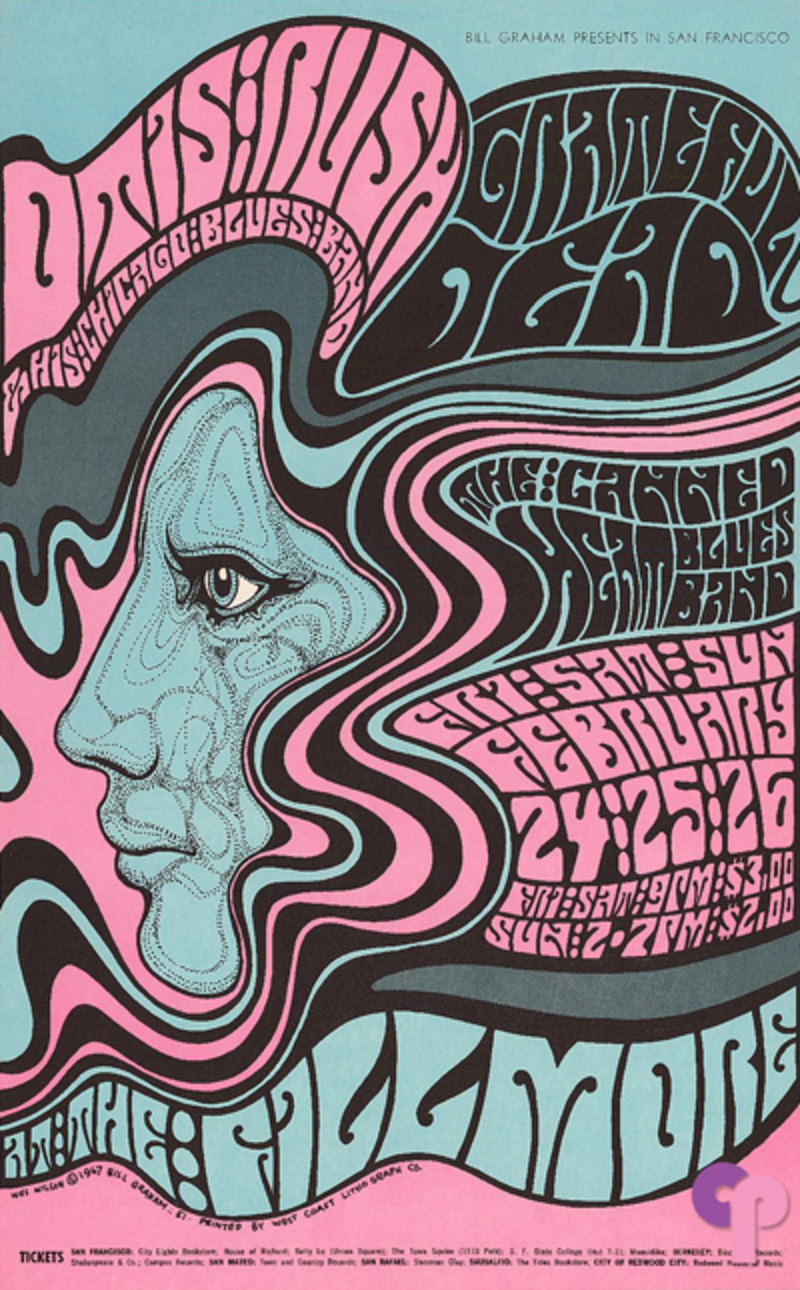
\includegraphics[width=0.4\linewidth]{figuras/posterTipo.pdf}
  \caption{Exemplo de tipografia aplicada como comunicação majoritariamente estética. Cartaz de Bill Graham feito para banda de \textit{Blues} de Chicago \citeC{graham2017}.}
  \label{fig:posterTipo}
\end{figure}


A tipografia também sofreu influências e foi moldada, tanto por limitações físicas como por correntes filosóficas adotadas pela sociedade. As limitações consistem no processo de fabricação dos tipos: metal, madeira, fotocomposição ou digital, sendo que cada um desses processos possui suas características próprias.


\section{Proposta de Projeto}

Tendo em vista que o deficiente visual possui pouco contato com a área, propõe-se um sistema auxiliar ao ensino de tipografia para deficientes visuais. Abre-se, então, a oportunidade de um novo tipo de leitura. Para o deficiente visual, abre-se um novo horizonte de conhecimento e interação dos invidentes com os caracteres latinos, usados em mais de um terço do mundo \citeC{World2015}. Ainda, a mitigação da exclusão cultural do deficiente visual, que é agravada pelo distanciamento desse grupo em relação ao elemento estético da tipografia.

Os deficientes visuais se encontravam em um ``gueto cultural'' antes do desenvolvimento de ferramentas como o \textit{DOSVOX} que possibilitassem a tradução dos textos escritos em braille para os caracteres latinos. Suas produções ficavam restritas já que raros videntes sabem ler ou escrever em braille e o acesso à informação ficava comprometido \citeC{Borges1998}. Nesse sentido, o projeto aqui proposto contribui também para a eliminação deste ``gueto cultural''.

Como já enfatizado, Neto \citeC{Neto2006} faz um trabalho voltado para responder a questão sobre qual é a influência que o uso das tecnologias assistivas de informação e comunicação tem sobre a experiência do deficiente visual com a escrita e com a leitura por meio do braille. Por outro lado, a proposta aqui apresentada estende esse objetivo ao tentar inserir o deficiente visual em um contexto que diz respeito, não somente aos caracteres utilizados pela língua nativa do país onde vive, mas também ensinar aspectos a respeito à anatomia de cada letra, permitindo diferenciar os caracteres entre si e os seus estilos, aproximando-o da experiência que um vidente tem ao ler qualquer mídia.

O sistema proposto possui não só um caráter de aproximação do invidente com a escrita e com os diversos estilos tipográficos, proporciona-lhe também a opção de se aprofundar nos estudos da tipografia, incluindo conceitos, aplicações e contextos históricos. Sendo assim, esse projeto apresenta um material inédito, por ser uma tecnologia assistiva que proporciona ao invidente o contato com uma informação antes restrita a ele, apesar de inicialmente ainda ser uma tecnologia com opções limitadas.

Além do mais, como o envolvimento dos deficientes visuais com o mundo digital da informática está crescendo, há necessidade de cursos formativos para que o invidente possa conhecer melhor as possibilidades de leitura e escrita utilizando as tecnologias assistivas desse natureza \citeC{Neto2006}. Sendo assim, um maior contato do deficiente com a tipografia é um fator predominante nesse contexto e que deve ser ensinado ao deficiente visual, sendo uma área ainda pouco explorada.

A proposta para esse projeto foi idealizada primeiramente por uma estudante de \textit{Design} da Universidade de Brasília, com a qual esse projeto foi desenvolvido em parceria. O projeto consiste em um sistema auxiliar para ensino de tipografia a deficientes visuais \citeC{Cruz2016}. O sistema, denominado Tipo Tátil, trata-se de um material tátil, com a qual o deficiente visual pode interagir e um material escrito, que traz as informações necessárias para auxiliar o ensino dessa área.

A parte tátil do sistema consiste de placas tridimensionais com as letras inseridas em alto relevo e réplicas avulsas, como ilustrado na Figura \ref{fig:placas}. Como prospota inicial, escolheram-se nove tipografias para compor o projeto, escolha baseada em uma classificação tipográfica específica (ver Capítulo \ref{ch:Tipografia}). Na Figura \ref{fig:tipografias}, apresentam-se as nove tipografias listadas, exemplificadas pelo caractere ``a'' como exemplo.

\begin{figure}[H]
 \centering
  \includegraphics[width=0.75\linewidth]{figuras/placasA.pdf}
  \caption{Conjunto de placas apresentando as nove tipografias \citeC{cruz2017}}
  \label{fig:placas}
\end{figure}

Esse sistema provê ao deficiente visual a diferenciação das características anatômicas e estilísticas de variados tipos, contando com o alfabeto completo para cada tipografia e também com um sistema pedagógico (material escrito) para que os deficientes visuais possam compreender as nuances e sutilezas da variedade de fontes tipográficas da escrita latina, entendendo seus significados formais e históricos \citeC{Cruz2016} \citeC{cruz2017}. Além disso, o projeto foi expandido para abarcar um exemplo de escrita cursiva, também apresentando placas com letras em alto relevo, bem como caracteres especiais de acentuação e operações matemáticas.

\begin{figure}[H]
 \centering
  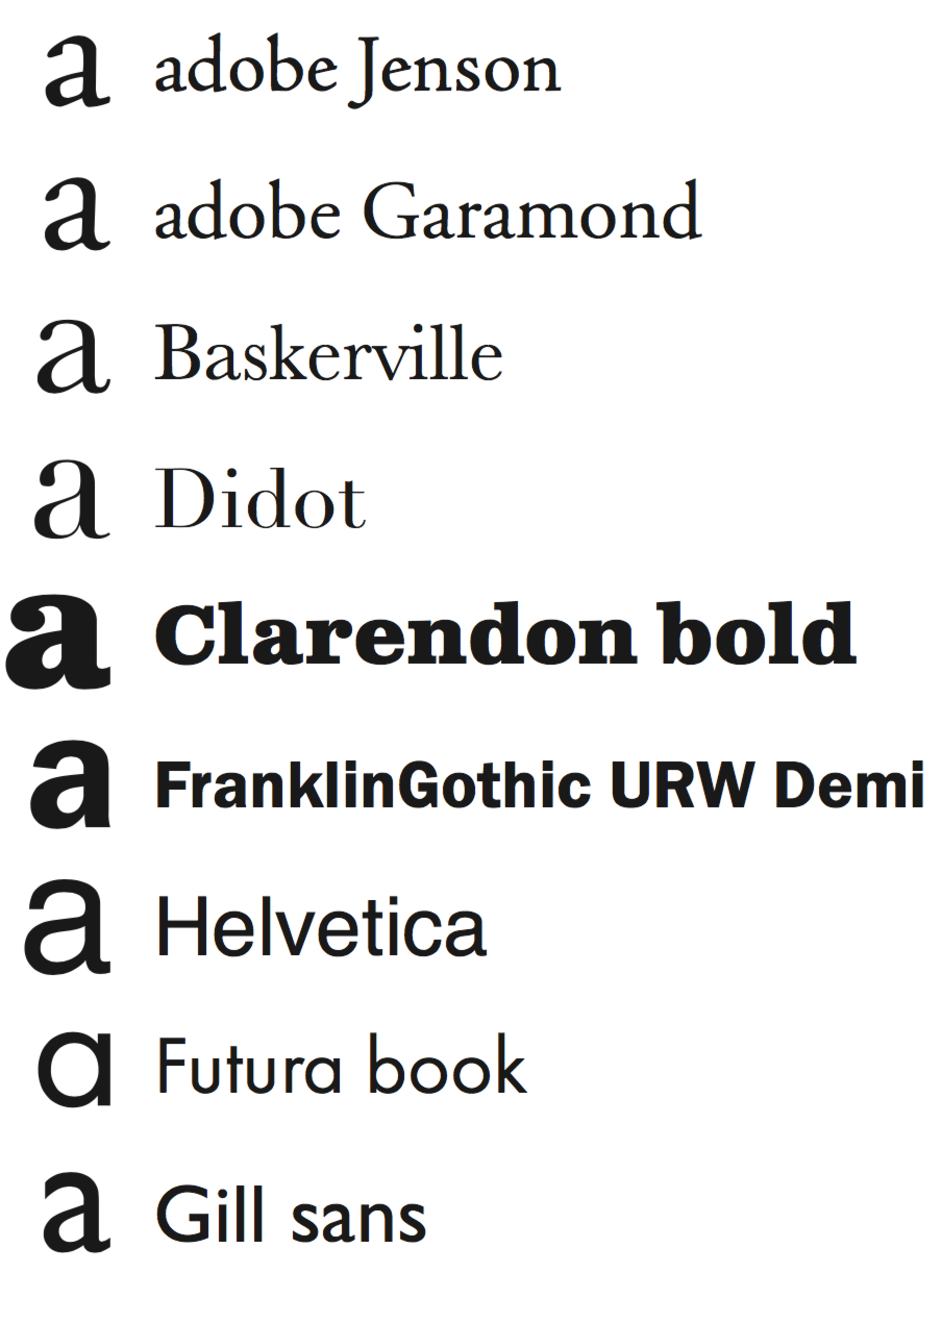
\includegraphics[width=0.4\linewidth]{figuras/tipografias.pdf}
  \caption{Tipografias que compõem o projeto.}
  \label{fig:tipografias}
\end{figure}


%Além disso,
De modo a tornar o projeto ainda mais completo, com o intuito de proporcionar ao deficiente a autonomia para estudar, de acordo com o conceito da tecnologia assistiva, e sabendo que maior eficácia é alcançada quando proporcionados estímulos multissensoriais, propõe-se a implementação de um sistema computacional auxiliar e interativo para guiar o deficiente visual durante o uso do produto de tecnologia assistiva \citeC{Ballestero-Alvarez2003}.

O sistema funcionaria com o usuário inserindo, em uma área pré-determinada, a peça sobre a qual deseja maiores informações. Então, a partir de captura de imagem (propõe-se uma \textit{webcam}) ocorreria o reconhecimento da tipografia e do caractere da peça e, por meio da síntese de voz, seriam providas ao usuário informações detalhadas sobre os conceitos acerca daquela tipografia, a saber, aplicações, especificações estilísticas e contexto histórico, conduzindo-o durante o processo de interação com a peça.

O escopo deste documento é o desenvolvimento e resultado da parte central do sistema: o algoritmo de reconhecimento de padrões que é utilizado para a classificação da tipografia da peça (tipo) contida em uma imagem de entrada (Figura \ref{fig:placas}).

Para o reconhecimento de padrões, serão empregadas técnicas de aprendizado de máquina (\textit{Machine Learning}). Geralmente essa é a melhor abordagem para se tratar problemas de reconhecimento de padrões, apesar de também haver a possibilidade de serem aplicadas outras técnicas como as heurísticas \citeC{Bishop2006}. Aprendizado de máquina é uma técnica pertencente ao campo da Inteligência Artificial e tem como objetivo obter sistemas capazes de aprender de forma automática, sem terem sido explicitamente programados \citeC{samuel1959} \citeC{ng2016}. O processo de aprendizado do sistema ocorre por meio de experiências e de soluções bem-sucedidas de casos anteriores \citeC{libralao2003}. As técnicas de aprendizado de máquina são aplicadas em problemas para extrair conceitos a partir de um banco de dados (reconhendo padrões). Sendo assim, a constituição do banco de dados (suficientemente grande) é uma parte importante do projeto e irá compor o conjunto de treinamento para o algoritmo de aprendizado de máquina.

O banco de dados, neste projeto, é formado por imagens contendo os diversos tipos. Sendo assim, as categorias das imagens são previamente conhecidas e rotuladas, sendo elas o nome de cada tipografia. Desta forma, o processo de aprendizado de máquina é denominado um problema de aprendizado supervisionado (\textit{supervised learning}).

Porém, em muitas aplicações, devido à grande variação dos dados de entrada, o algoritmo compreende apenas uma pequena porção de todo o conjunto que deseja-se classificar. Sendo assim, uma prática comum é passar os dados (neste caso, as imagens) por um método de pré-processamento, de forma a uniformizar as imagens de entrada. Um exemplo do processo adotado em um algoritmo de reconhecimento óptico de caracteres (OCR, \textit{Optical Character Recognition}, em inglês) é apresentado na Figura \ref{fig:etapas}. Está é uma abordagem comum para a solução desse tipo de problema, sendo um caso semelhante ao aqui proposto \citeC{Bishop2006} \citeC{Miranda2013}.

Os classificadores empregados neste projeto são a Máquina de Vetor de Suporte (SVM, em inglês \textit{Support Vector Machine}) e a Floresta Aleatória (\textit{Random Forest Classifier}). Máquina de Vetor de Suporte é um modelo classificador paramétrico, baseado na Teoria de Aprendizado Estatístico, podendo ser usada em casos de classificação ou regressão linear \citeC{lorena2007}. Já a Floresta Aleatória é uma extensão do modelo de Árvores de Regressão e de Classificação e sua predição baseia-se em dividir recursivamente o conjunto de dados, com base nos valores de preditores \citeC{maindonald2007}.

\begin{figure}[H]
  \centering
  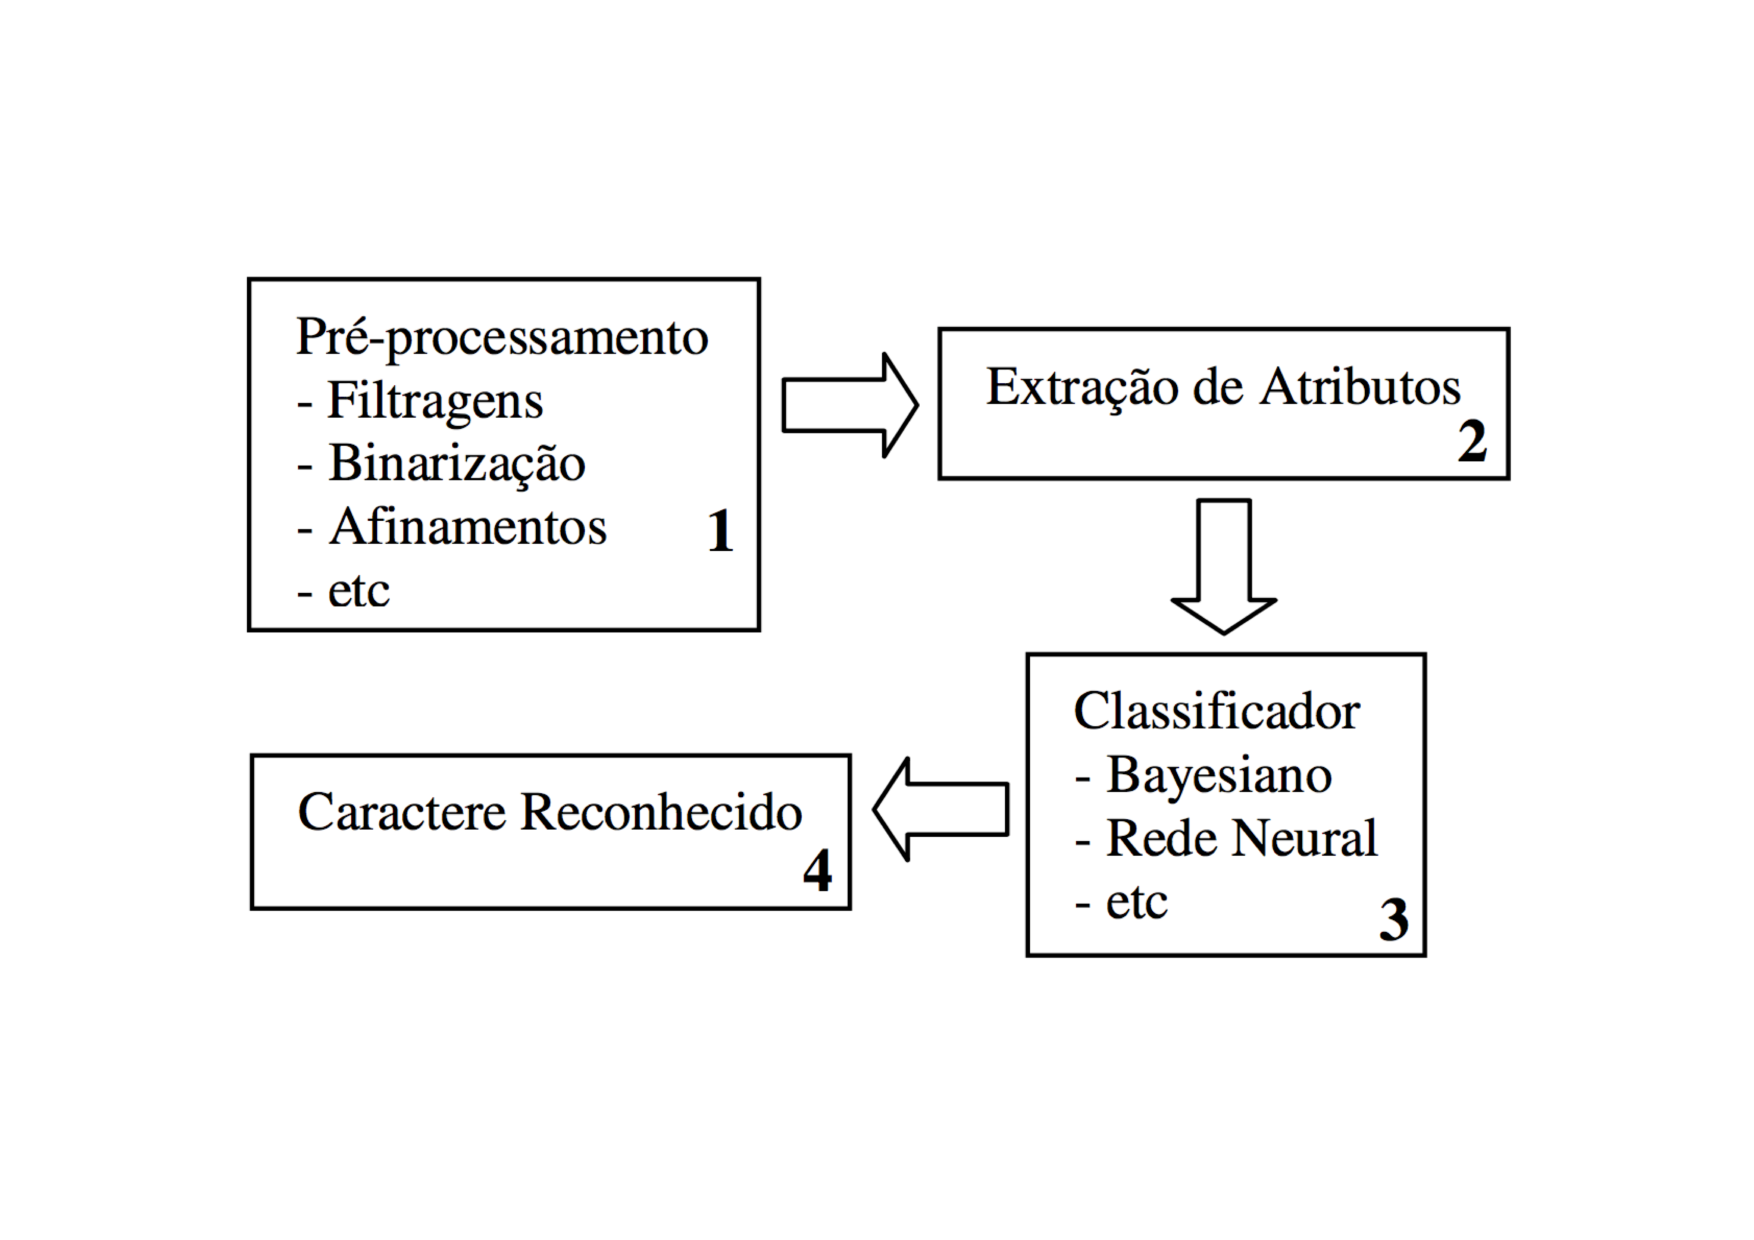
\includegraphics[width=0.7\linewidth]{figuras/etapaProcessamento.pdf}
  \caption{Etapas do Processo de Reconhecimento de Caracteres \citeC{miranda2013handwritten}}
  \label{fig:etapas}
\end{figure}

Vários dos softwares de tecnologia assitiva utilizam OCR em sua composição para leitura de tela ou de arquivos. Entre os exemplos, podem-se citar o \textit{OpenBook}, o \textit{Jaws} e o \textit{Virtual Vision} \citeC{OpenBook2016} \citeC{Jaws2016} \citeC{VV2016}. No sistema de auxílio ao ensino da escrita à mão para deficientes visuais proposto por Plimmer \citeC{Plimmer2008}, também utiliza-se OCR e uma abordagem semelhante à de Miranda \citeC{Miranda2013}. Desta forma, percebe-se que esse campo de reconhecimento de caracteres favorece o desenvolvimento de várias tecnologias assistivas.

Apesar de o reconhecimento de padrões ter raízes históricas na ciência, a sua abordagem com aprendizado de máquina encontra-se em um momento ímpar de crescimento. Graças ao veloz crescimento e popularização dos dispositivos com câmera, como smartphones e tablets, e também da internet e redes sociais, o volume de imagens e vídeos compartilhados na rede é imenso. Além disso, a capacidade de processamento dos computadores também apresenta um crescimento acelerado. Dessa forma, o aprendizado de máquina enfrenta um ótimo momento  para seu desenvolvimento, já que está acessível um grande banco de dados de imagens para compor o conjunto de treinamento e o hardware necessário para o processamento também \citeC{Feris2016}. Sendo assim, várias são as aplicações nessa área, desde utilidades no campo das ciências sociais até o campo da criminalística \citeC{Grimmer2015} \citeC{li2015clothing}. Para o reconhecimento de padrões na área de Visão Comuputacional, o aprendizado de máquina é muito importante, sendo aplicado em várias situações como, por exemplo, na localização de prédios, no reconhecimento facial e na edição inteligente de fotos \citeC{szeliski2010computer}.

Por outro lado, o reconhecimento de tipos (OFR, \textit{Optical Font Recognition}, em inglês) continua como um campo que não é muito explorado pela comunidade de pesquisadores \citeC{Zramdini1995}. Geralmente, quando o problema é atacado, utiliza-se o reconhecimento de tipos apenas como forma de melhoria para o reconhecimento de caracteres, especialmente quando um documento possui variadas tipografias, ou ainda para uma possível classificação de documentos, que podem ser diferenciados de acordo com a tipografia ali empregada \citeC{Shi1997} \citeC{Manna1999}. Outra situação na qual o reconhecimento de fontes é utilizado é no reconhecimento de caracteres não-latinos, como chineses, arábicos ou farsi \citeC{Yang2006} \citeC{Slimane2013} \citeC{Zahedi2011}.

Nesse contexto, o trabalho de Zramdini \citeC{Zramdini1995} tem como diferencial um sistema que considera todas as variedades anatômicas e intrafamiliares das fontes e por também propor uma combinação entre o reconhecimento de fontes e de caracteres, o que faz parte do objetivo do sistema final proposto para o projeto apresentado neste documento. No entanto, Zramdini \citeC{Zramdini1995} apresenta uma abordagem distinta da aplicada nesse projeto para o reconhecimento das tipografias. Em seu trabalho, o autor utiliza as características dos caracteres, baseadas em propriedades locais das letras individuais, tais como a anatomia de cada letra e as peculiaridades de determinadas tipografias. Por exemplo, uma das características utilizadas é o estilo de serifa, para estimá-lo, computa-se a borda de cada caractere e analisa-se o comprimento da borda, para determinar o estilo da serifa. Uma das restrições deste trabalho \citeC{Zramdini1995} é que, para que possa ocorrer a classificação de tipografia baseada em comparações estruturais entre os tipos, deve-se ter um conhecimento prévio em relação à qual classe o caractere avaliado pertence. Sendo asim, o autor desenvolveu um sistema classificador distinto para cada caractere. Este sistema primeiramente aplica um algoritmo de OCR para identificar o caractere e, posteriormente, o modelo classificador para classificar a tipografia (OFR).

Já no caso do projeto apresentado neste trabalho, os caracteres foram tratados simplesmente como imagens, não sendo um requisito o conhecimento prévio em relação à qual carecetere se trata. Os seus atributos foram extraídos, também de forma local, por meio do Padrão Binário Local (LBP, \textit{Local Binary Pattern} em inglês), um operador proposto em 1994 e utilizado em visão computacional, especialmente em classificação de texturas e reconhecimento de faces \citeC{ojala1994} \citeC{do2012}.

\section{Estrutura do Trabalho}

Este documento divide-se de forma a apresentar uma estrutura que facilite o entendimento do leitor em relação ao desenvolvimento do sistema de reconhecimento de padrões em tipos para classificação das tipografias presentes no projeto explicitado na seção anterior. No Capítulo \ref{ch:Tipografia}, apresentam-se conceitos básicos de tipografia, relevantes para o projeto. No Capítulo \ref{ch:ML} são explicados os fundamentos teóricos dos modelos de extração de atributos e de classificação, bem como a estrutura do algoritmo de Aprendizado de Máquina.

Já nos Capítulos seguintes, a saber, \ref{ch:Metodologia} e \ref{ch:Resultados}, é detalhado o desenvolvimento do trabalho especificamente, com todos os algoritmos implementados na metodologia e os resultados alcançados, bem como sua análise. No Capítulo \ref{ch:Conclusao}, apresentam-se as conclusões e discutem-se quais os objetivos do projeto já foram alcançados e quais serão os passos futuros.


%\begin{figure}[H]
%  \centering
%  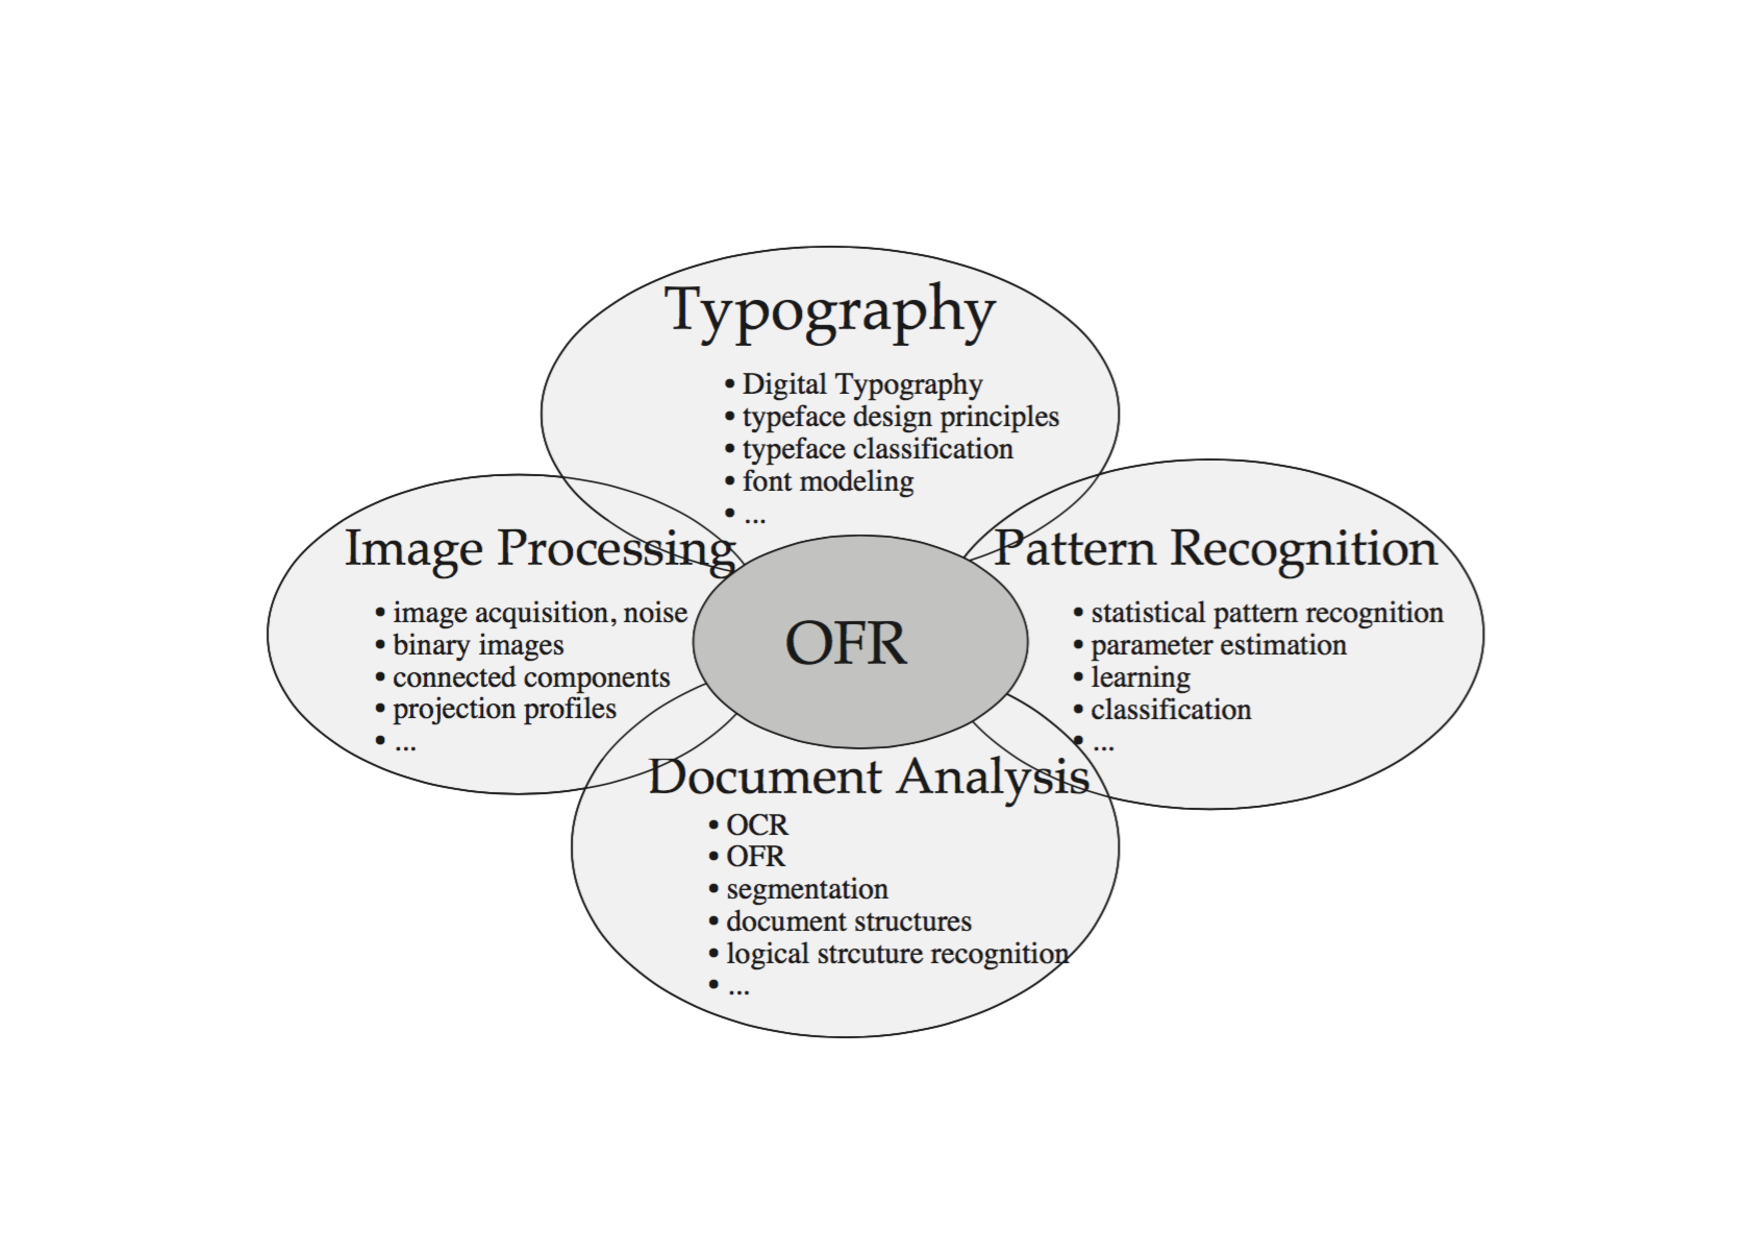
\includegraphics[width=0.8\linewidth]{figuras/OFRareas.pdf}
%  \caption{Áreas Necessárias para Reconhecimento de Fontes - \textbf{Fonte:} \citeC{Zramdini1995}}
%  \label{fig:OFRareas}
%\end{figure}



%for the recognition of characters, but the rec- ognitionofthetypeoffontsisdisregarded \citeC{aviles2005}
%The methodology applied in our processing im- age algorithm was based on to estimate features not over full image, instead of this, feature estima- tionwasdoneoverregionsofimagescalled‘‘sub- image’’.Theestimatedattributearraysofeach sub-image were the reference database to recognize thetypeofeachfont(100windowsaretakenran- domlyovereachfulltext) \citeC{aviles2005}



%Uma citação~\cite{artigo:2015}.

%As citações são feitas usando o comando~\texttt{\textbackslash cite}. Para usar colchetes nas citações, use o comando~\texttt{\textbackslash citeC}. Exemplo \citeC{artigo:2015}.


%blá blá, blá \cite{artigo:2015}

\chapter{Sobre Tipografia}
\label{ch:Tipografia}

\section{Tipografia}

tipografia blablablabla

Tipografia é comunicação escrita por meio de tipos (BIERUT, M., HELFAND, J., HELLER, S. AND POYNOR, R., 2010) surgiu na Alemanha na década de 1450, quando aliaram-se os tipos móveis de metal à prensa resultando no primeiro livro impresso (BRINGHURST, 2011).  A diferença entre a letra escrita e a tipográfica é o método como são geradas, independente do resultado final aparente (Smeijers, 2011). Por exemplo, existem fontes cursivas. Na era digital os tipos móveis foram adaptados para o que chamamos de fontes.


as classificações tipográficas surgiram com a intenção de  criar uniformidade na definição e descrição dos tipos. Ainda que não exista uma classificação oficial na área da tipografia, a classificação criada por maximilien vox e adaptada posteriormente pela ATypl, é uma das classificações mais reconhecidas e utilizadas. Ela une características históricas e estéticas e é dividida em grupos e subgrupos(ROCHA, 2012).

\chapter{Reconhecimento de Padrões e Aprendizado de Máquina}
\label{ch:ML}

Este capítulo é destinado à apresentação da fundamentação teórica dos conceitos gerais de reconhecimento de padrões e dos algoritmos de aprendizado de máquina utilizados neste projeto. Também são detalhados os processos utilizados no pré-processamento dos dados de treinamento (imagens) e na extração de atributos que estão relacionados ao desenvolvimento do sistema.

%na etapa de construção do banco de dados,

\section{Conceitos Gerais}

O príncipio sobre o qual o Aprendizado de Máquina opera é a indução, na qual, a partir de um conjunto de casos (exemplos) que tipificam o problema, são feitas generalizações e, então, decisões são tomadas baseadas nessa regra construída. Para tal, necessita-se de um conjunto de dados de treinamento, que desempenham o papel dos exemplos para indução e um modelo de Aprendizado de Máquina, que irá ser ajustado conforme padrões apresentados nos dados de treinamento.

Como já descrito brevemente no Capítulo \ref{ch:intro}, o aprendizado indutivo da máquina pode ocorrer como aprendizado supervisionado (\textit{supervised learning}) ou aprendizado não-supervisionado (\textit{unsupervised learning}). O último caracteriza-se por utilizar um conjunto de dados para os quais não existem classes pré-definidas, então, as classes são formadas durante o treinamento da máquina, sendo os domínios divididos naturalmente. Essa divisão é feita a partir da análise de padrões nos dados (imagens) como regiões com alta densidade relativa de pontos no espaço \citeC{perottoalvares2005}.

Já o aprendizado supervisionado, como no caso deste projeto, se dá com um conjunto de dados de treinamento que possuem classes já definidas e, portanto, tem-se uma estrutura na seguinte forma: entrada e saída desejada. As classes são apresentadas como rótulos de cada amostra do conjunto de dados e todo esse processo de aprendizado supervisionado é mostrado na Figura \ref{fig:supervised}, na qual o conjunto de exemplos rotulados apresentam a forma $(\boldsymbol{x_i}, y_i)$, em que $\boldsymbol{x_i}$ é o vetor de uma amostra e $y_i$ é seu rótulo. O classificador obtido por meio do algoritmo de aprendizado de máquina é denotado como $f$. Neste exemplo, tem-se um conjunto de $n$ dados, onde cada dado $\boldsymbol{x_i}$ possui $m$ atributos.

\begin{figure}[H]
 \centering
  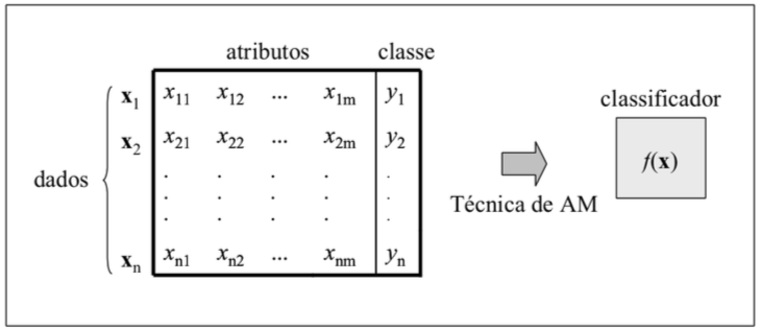
\includegraphics[width=0.8\linewidth]{figuras/supervisedLearning.pdf}
  \caption{Processo de treinamento de modelo classificador com aprendizado supervisionado \citeC{lorena2007}.}
  \label{fig:supervised}
\end{figure}

Os exemplos do conjunto de treinamento são representados como atributos em um vetor, sendo que cada atributo expressa uma característica do dado, a qual é utilizada no treinamento do modelo de aprendizado de máquina. Os tipos de atributos são o nominal e o contínuo. O primeiro tipo (nominal) gera um problema de classificação, no qual o objetivo é atribuir a cada vetor de entrada uma das categorias finitas (valores discretos). Este é o tipo de problema apresentado neste projeto. O tipo contínuo de atributo corresponde a um caso de regressão, em que à saída desejada é atribuída uma ou mais variáveis contínuas. Um exemplo é o problema de predição do preço de uma casa, que pode utilizar atributos como o tamanho e a localização da casa \citeC{Bishop2006}.

O classificador também utiliza uma função para descrever os dados. Sendo assim, é utilizada uma parte do conjunto de dados, denominada conjunto de teste, para mensurar o grau de desempenho do modelo de predição. Neste projeto, para avaliação do desempenho e da capacidade de generalização do modelo utiliza-se a técnica de Validação Cruzada (\textit{Cross Validation}). Nesta técnica, divide-se o conjunto total de dados em vários subconjuntos, sendo alguns utilizados para estimação dos parâmetros do modelo (etapa de treinamento) e outros, para a validação \citeC{kohavi1995}. Os três métodos mais populares de Validação Cruzada são: K-Pastas (\textit{K-Fold}), Substituição da Amostra (\textit{Holdout}) e Deixe-Um-De-Fora (\textit{Leave-One-Out}), sendo o primeiro escolhido para a implementação do sistema aqui apresentado \citeC{gonzalez2013}.

No método K-Pastas, o conjunto de dados é dividido aleatoriamente em $k$ subconjuntos, sendo um subconjunto destinado para teste e $k-1$ subconjuntos, para treinamento. O processo de treinamento do modelo classificador e de avaliação de seu desempenho é realizado $k$ vezes, sendo que, a cada vez que o processo é repetido, faz-se uma nova divisão do conjunto total em subconjuntos. Então, o desempenho final do classificador é obtido calculando-se a média de $k$ avaliações \citeC{schneider1997}.

%\section{Métodos Utilizados na Composição do Banco de Imagens e na Etapa de Pré-Processamento}

\section{Extração de Atributos}

Para o treinamento do algoritmo classificador são necessários atributos dos dados do conjunto de treinamento. A extração de atributos está relacionada com a redução da dimensionalidade de dados. Além de serem parâmetros descritivos do dado ao qual pertence, os atributos evitam que a quantidade de dados de entrada para o treinamento do modelo seja excessivamente grande, o que aumentaria o esforço computacional.

Desta forma, o problema de super-ajustamento (\textit{overfitting}) às amostras no treinamento pode ser evitado com a correta seleção de atributos.  O super-ajustamento pode ser causado por uma grande quantidade de variáveis no modelo, sendo definido como uma demasiada especialização nos dados de treinamento e, consequentemente, uma generalização ruim que gera uma baixa taxa de acerto para dados de entrada diferentes dos de treinamento \citeC{lorena2007}.

Também pode ocorrer um caso de sub-ajustamento (\textit{underfitting}), o que produz uma taxa de acerto que pode ser também considerada baixa para esta aplicação. O sub-ajustamento, por sua vez, é quando o modelo treinado não descreve bem o conjunto de dados de treinamento, apresentando baixa e insuficiente especialização em relação a esses dados. O sub-ajustamento em geral se deve à escolha de atributos pouco representativos para o tipo de análise pretendida.

Conclui-se, então, que a etapa de extração de atributos é importante para o bom desempenho do classificador. Neste projeto, a extração de atributos das imagens de entrada foi feita utilizando o operador Padrão Binário Local (LBP, \textit{Local Binary Pattern} em inglês). Os vetores de atributos são formados concatenando-se os histogramas das imagens resultados da aplicação do LBP, o qual é descrito a seguir.


\subsection{Padrão Binário Local (LBP)}

O operador LBP se popularizou devido à sua simplicidade computacional, que possui pouca sensibilidade à variação de iluminação e invariância à rotação. Esse operador, quando aplicado em uma imagem, substitui cada pixel (central) por um valor binário, que é obtido por meio da comparação desse pixel com seus vizinhos. Mais especificamente, forma-se uma matriz de nove pixels, no qual o pixel central é comparado com todos os oito pixels vizinhos ao pixel central. Para os pixels com valor maior do que o pixel central, atribui-se "1", caso contrário, atribui-se "0". Após esse processo, um número binário é gerado, considerando que a matriz foi avaliada em sentido horário, com o primeiro pixel sendo o bit menos significativo. Uma ilustração da aplicação do operador LBP em um pixel de uma imagem é apresentada na Figura \ref{fig:lbpTeoria}. Neste exemplo, qual o valor resultante gerado após a aplicação do LBP é 184 \citeC{do2012}. Em segundo momento na Figura \ref{fig:lbpTeoria}, mostra-se a imagem resultante após a aplicação do LBP.

\begin{figure}[H]
 \centering
  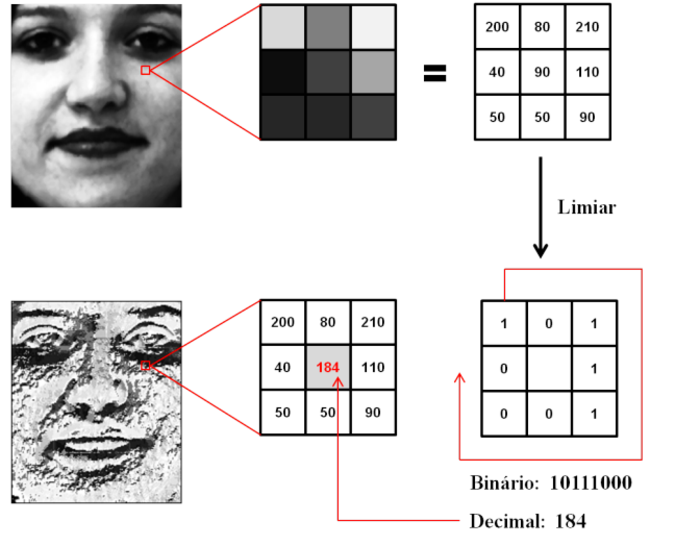
\includegraphics[width=0.65\linewidth]{figuras/lbpTeoria.pdf}
  \caption{Processo do operador LBP em um pixel \citeC{do2012}}
  \label{fig:lbpTeoria}
\end{figure}

Naturalmente, o LBP pode ser computado em áreas maiores do que 3x3 pixels. Neste caso, cria-se uma circunferência de raio $R$, que pode ser ajustado. Também se determina o número de pontos amostrais $P$ sobre a circunferência. A comparação se dá entre o pixel principal central e as posições amostradas no círculo com a imagem interpolada. Este procedimento é ilustrado ilustrado na Figura \ref{fig:lbpTeoria2} para alguns valores de P e R.


\begin{figure}[H]
 \centering
  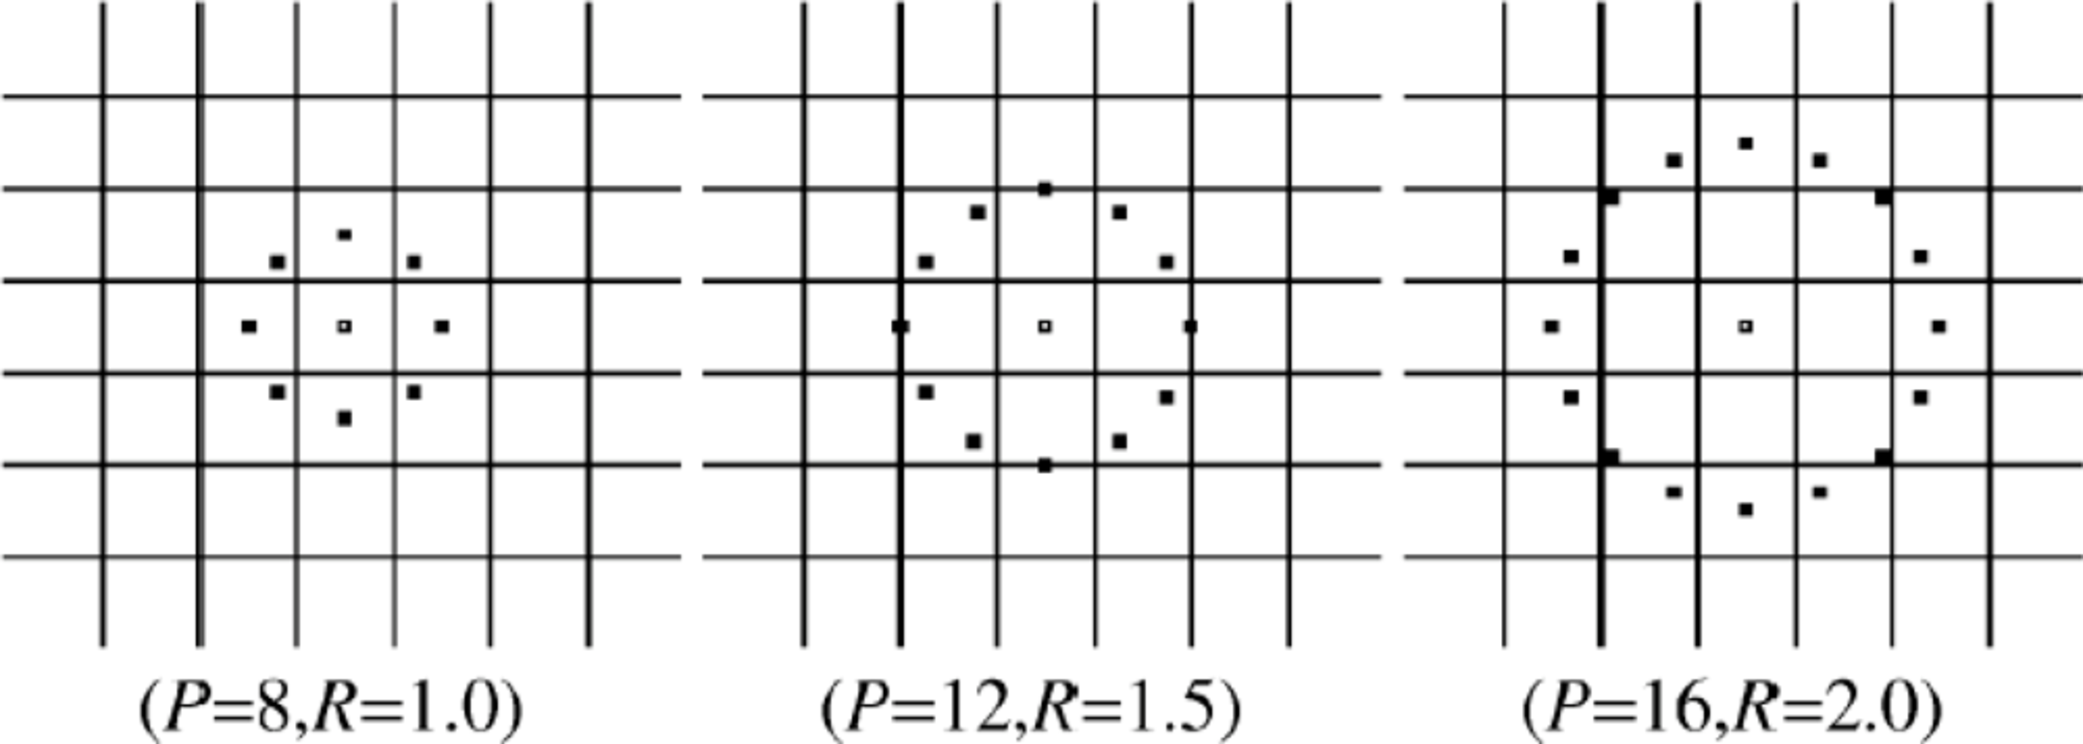
\includegraphics[width=0.65\linewidth]{figuras/lbpRP.pdf}
  \caption{Exemplo de operador LBP com diferentes valores de $P$ e $R$ \citeC{zhao2011}}
  \label{fig:lbpTeoria2}
\end{figure}

A seguinte equação define o operador LBP nos termos de $R$, $P$ e os valores em escala de cinza dos pixels da imagem:

\begin{equation}
\label{eq:eqLBP}
 LBP_{P,R}
   \begin{cases}
    \displaystyle\sum_{p=0}^{P-1}S(g_p - g_c)  & \quad \text{se número de transições} \leq 2 \\
    P+1  & \quad \text{caso contrário } \\
   \end{cases}
\end{equation}

 Sendo $g_c$ o valor do pixel central e $g_p$, o do pixel que está sendo comparado. Assim, obtém-se a sequência de valor binário $T_p={S(g_0 - g_c), ...,S(g_{P-1} - g_c)}$, em que $S(x) = 0$ se $x < 0$ e é igual a 1 caso contrário \citeC{muscipadroes}.

Para tornar o operador LBP invariante à rotação, pode-se modificar a ordem com que coleta-se os bits, de forma a alterar a sua representação binária. Mais especificamente, escolhemos como a primeira posição entre os pontos amostrais aquela que gera o menor valor final. Isso faz com que a possibilidade de valores para o LBP seja de 36 variações no total \citeC{prince2012}.

Pode também haver uma predominância da ocorrência de valores binários considerados uniformes, ou seja, aqueles em que são poucas, ou inexistentes, as transições de 0 para 1. Desta forma, a quantidade de classes de texturas pode ser reduzida quando agrupam-se todos os LBPs não-uniformes em uma única classe.

De forma geral, após o cálculo do LBP para todos os pixels da imagem, calcula-se o histograma desta nova imagem. O histograma é um descritor com a principal função de apresentar de forma compacta as características da imagem. O histograma usado para o LBP, enquanto uma função discreta, pode ser descrito pela seguinte equação:

\begin{equation}
\label{eq:eqHist}
  h(r_k)=n_k
\end{equation}

Onde $r_k$ é o valor de uma das classes do LBP e $n_k$ é a quantidade de pixels que apresentam o referido valor do LBP \citeC{gonzalezwoods2014}.

No entanto, é comum utilizar a versão normalizada do histograma que é descrita por:

\begin{equation}
\label{eq:eqHistNorm}
  p(r_k)=\frac{n_k}{MN}
\end{equation}

Em que M e N representam as dimensões da imagem.

Sendo assim, ao final do processo, todos os histogramas da imagem são concatenados ao final do processo, de forma a se tornarem um único vetor de atributos daquela imagem.

\section{Classificadores}

Os atributos extraídos das imagens do conjunto formam vetores, um para cada imagem, de forma a caracterizá-las. Esses são os dados de entrada para o modelo classificador. As características destes dados de entrada são analisados na fase de treinamento do modelo para ajustar o classificador, de forma que ele consiga realizar a classificação correta de novos dados de entrada.

Neste projeto, os modelos escolhidos para classificação no sistema foram: Máquina de Vetor de Suporte (SVM, em inglês \textit{Support Vector Machine}) em primeiro momento e, posteriormente, a Floresta Aleatória (\textit{Random Forest Classifier}). Ambos são apresentados mais detalhadamente nas seções seguintes.

\subsection{Máquina de Vetor de Suporte}

As Máquinas de Vetor de Suporte são um modelo de aprendizado com grande popularidade na comunidade de Aprendizado de Máquina. A SVM é utilizada em variadas aplicações, desde bioinformática ao reconhecimento de imagens, como é o caso desse projeto \citeC{mitchell1997} \citeC{noble2004} \citeC{kim2002}.

Intrinsicamente, a SVM é um modelo de classificação binária em problemas de aprendizado supervisionado (\textit{supervised learning}). Concedido um conjunto de dados para treinamento, todos especificados como pertencendo a uma das duas categorias, o treinamento do algoritmo SVM gera um modelo que irá classificar novos dados como sendo de uma categoria ou de outra.

A SVM baseia-se em um mapeamento de todos os dados de treinamento, representando-os como pontos em um espaço. Os exemplos para treinamento são divididos nesse espaço de acordo com sua categoria de tal forma que os dois conjuntos de pontos estejam distanciados pelo maior espaçamento possível (d), como ilustrado na Figura \ref{fig:svmDist}. Sendo assim, um novo dado, quando fornecido ao sistema, é mapeado nesse mesmo espaço e a predição de sua classe é feita de acordo com a sua localização no espaço, que foi gerado no treinamento do modelo.

\begin{figure}[H]
 \centering
  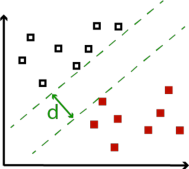
\includegraphics[width=0.4\linewidth]{figuras/svmDist.pdf}
  \caption{Ilustração da distância dos subconjuntos de dados de treinamento mapeados no espaço pelo modelo SVM.}
  \label{fig:svmDist}
\end{figure}

Em sua versão linear, a SVM pode ser classificada como "Margens Rígidas" ou "Margens Suaves". Em ambos casos, definem-se fronteiras lineares (para aplicação do limiar de decisão) no conjunto de dados que aprensentam perfil linearmente separável. As margens são utilizadas na SVM para encontrar a solução de classificação para os subconjuntos de forma que o erro de generalização seja o menor possível. Desta forma, as margens são definidas como a menor distância entre o hiperplano (fronteira) de decisão e qualquer uma das amostras de treinamento \citeC{Bishop2006}.

No entanto, apesar de não se aplicar a este projeto, a SVM também pode ser empregada em problemas em que os dados de treinamento não são rotulados, ou seja, em caso de aprendizado não-supervisionado (\textit{unsupervised learning}). Para tal, há uma versão distinta da SVM que funciona baseada no mapeamento dos dados em um espaço. No entanto, inicialmente realiza-se um processo para encontrar as conexões naturais entre os dados de entrada, formando grupos de acordo com o grau de similaridade apresentado entre eles, para então distribuí-los no espaço. Essa técnica é um algoritmo de aglomeração (\textit{clustering}) conhecido como \textit{Support Vector Clustering} \citeC{ben2001}.

\subsubsection{SVM com Margens Rígidas}

Pode-se definir um conjunto de dados de treinamento \textit{C}, composto de dados \textit{$x_i$} $\in$ X, no qual \textit{i $=$ 1, ..., n} e X é o espaço de dados, cujos rótulos de categoria são \textit{$y_i$} $\in$ Y, onde Y = \{$-$1,$+$1\}. Sendo assim, o conjunto \textit{C} é dito linearmente separável caso possa-se criar um hiperplano tal que os subconjuntos de dados com valor $-$1 seja separado do subconjunto de dados $+$1 \citeC{lorena2007}.

A seguinte equação, representa um hiperplano qualquer e divide o espaço dos dados de treinamento em duas regiões, uma para representar $-$1 e outra, $+$1,

\begin{equation}
\label{eq:eqHiper}
 f(x)= \boldsymbol{w}\cdot \boldsymbol{x} + b = 0
\end{equation}


Desta forma, define-se uma função \textit{$g(x)$} como a função sinal de \textit{$f(x)$} que irá ser o padrão para a classificação de novos dados de entrada, dada pela seguinte equação:


\begin{equation}
\label{eq:eqSgn}
 g(x) = sgn(f(x)) =
   \begin{cases}
    +1       & \quad \text{se } w\cdot x + b \text{ } $>$ \text{ } 0\\
    -1  & \quad \text{se } w\cdot x + b \text{ } $<$ \text{ } 0\\
   \end{cases}
\end{equation}

na qual $\boldsymbol{w}$ é o vetor normal ao hiperplano criado.

Para $f(x) = 0$, a distância entre um ponto no espaço (amostra) e o hiperplano definido é dada por $|f(x)| \mathbin{/} ||w||$. Além disso, deve existir pelo menos um conjunto de parâmetros $\boldsymbol{w}$ e \textit{b} que satisfaça \textit{g(x)}, ou seja, tal que \textit{$y_i$ $\cdot$ $f(x_i)$ $>$ 0}. Sendo assim, pode-se definir a distância entre uma amostra $x_i$ qualquer e o hiperplano escolhido como na seguinte equação:

 \begin{equation}
\label{eq:eqDist}
  \frac{y_i \cdot f(x_i)}{||\boldsymbol{w}||} = \frac{y_i(\boldsymbol{w} \cdot x_i + b)}{||\boldsymbol{w}||}.
\end{equation}

As margens ($H_1$ e $H_2$) são definidas, em primeiro momento, mediante a distância perpendicular entre a fronteira de decisão e aquele que é o ponto mais próximo de todas as amostras dos dados de treinamento, como mostra a parte \textit{a} da Figura \ref{fig:marginSVM}. Posteriormente, as margens são maximizadas escolhendo-se a sua localização, tomando como base as amostras que se encontram mais próximas do hiperplano separador, como destacado na parte \textit{b} da Figura \ref{fig:marginSVM}. Essas amostras são denominadas Vetores de Suporte (\textit{support vectors}), dando nome à técnica de aprendizado. Para maximizar a distância entre os vetores de suporte e o hiperplano separador ($f(x) = 0$), deve-se otimizar os parâmetros $\boldsymbol{w}$ e \textit{b}, que são ajustados durante o treinamento do modelo \citeC{rosebrock2017}.

\begin{figure}[H]
 \centering
  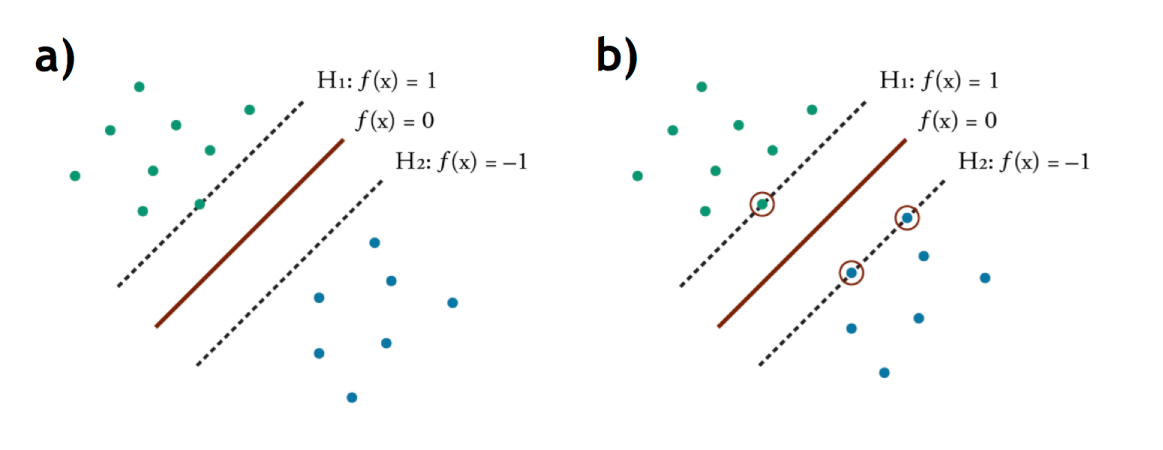
\includegraphics[width=0.9\linewidth]{figuras/marginSVM.pdf}
  \caption{Ilustração do hiperplano separador e do estabelecimento das margens ($H_1$ e $H_2$) no espaço em que os dados de treinamentos estão mapeados.}
  \label{fig:marginSVM}
\end{figure}

Realizando um escalonamento, a partir de uma mesma constante em termos de $\boldsymbol{w}$ e em \textit{b} não altera-se a distância dos pontos $x_i$ em relação ao hiperplano separador, a expressão $y_i(\boldsymbol{w} \cdot x_i + b)$ pode ser considerada unitária. Desta forma, a distância mínima entre o hiperplano e os dados de treinamento é de $1/||w||$. Busca-se, então, maximizar essa distância com a minimização de $||w||$, valendo-se do problema de otimização na expressão seguinte

\begin{equation}
\label{eq:eqMin}
  \text{min}\{\frac{1}{2}||\boldsymbol{w}||^2\},
\end{equation}

onde são consideradas as seguintes restrições

\begin{equation}
\label{eq:eqRestrição}
  \text{Restrições: } y_i(\boldsymbol{w} \cdot x_i + b) \geq 1, i \in (1,n)
\end{equation}

de forma a garantir que não haverão dados de treinamento entre as margens de separação de classes, daí então a nomenclatura "margens rígidas" \citeC{lorena2007}.

Esta é uma importante propriedade da SVM, tornando a determinação dos parâmetros do modelo uma otimização convexa, na qual a solução mínima é obrigatoriamente a solução global \citeC{Bishop2006}.

Para solucionar o problema de otimização da equação \ref{eq:eqMin}, pode ser utilizada uma função Lagrangiana, associando parâmetros $a_i$ (multiplicadores de Lagrange) e tornando suas derivadas parciais nulas. A resolução completa deste problema pode ser encontrada nas referências \citeC{Bishop2006} e \citeC{lorena2007}. Valendo-se do resultado dessa operação, tem-se a definição da função utilizada para a classificação dos dados que serão fornecidos ao sistema, dada pela seguinte equação

\begin{equation}
\label{eq:eqSVM}
  g(x) = sgn(f(x)) = sgn\left(\displaystyle\sum_{i=1}^{n}a_iy_ik(\boldsymbol{x},\boldsymbol{x_i})+b\right)
\end{equation}

sendo a função sinal do resultado da função de Lagrange aplicada nesse caso.

Pode-se perceber que na Equação \ref{eq:eqSVM} empregou-se o conceito de \textit{kernel} na resolução final do problema de otimização. Define-se a função \textit{kernel} como $k(x,x') = \phi(\boldsymbol{x})^T\phi(\boldsymbol{x'})$, na qual $\phi(\boldsymbol{x})$ indica um mapeamento, ou transformação, para um determinado espaço de características (\textit{feature space}), $\phi:X\mapsto\eth$. Apesar de, com o uso da função \textit{kernel} na formulação, o esforço computacional tornar-se mais elevado, dá-se flexibilidade ao modelo que pode ser reformulado usando diferentes tipos de \textit{kernel} e, então, pode ser aplicado em outros casos nos quais a dimensionalidade excede o número de amostras de treinamento \citeC{Bishop2006}.

\subsubsection{SVM com Margens Suaves}

A SVM com Margens Suaves é uma adaptação da versão do algoritmo com Margens Rígidas para que o aprendizado seja mais eficiente em casos de dados reais, os quais, comumente, não se apresentam conjuntos de dados estritamente bem comportados, ou seja, linearmente separáveis. Com essa versão da SVM, propõe-se lidar com conjuntos de treinamento mais gerais. Para isso, exceções às restrições apresentadas na expressão \ref{eq:eqRestrição}. Sendo assim, são estabelecidas variáveis de folga ($\xi_i$, $i \in (1,n)$) e são adicionadas ao problema e a equação \ref{eq:eqRestrição} é modificada para:

\begin{equation}
\label{eq:eqSuave}
 y_i(\boldsymbol{w} \cdot x_i + b) \geq 1 - \xi_i, \text{ } \xi_i > 0, \text{ } i \in (1,n).
\end{equation}

O efeito dessa modificação é que, devido a essa folga adicional, alguns pontos dos dados de treinamento podem permancer entre as margens $H_1$ e $H_2$. Por outro lado, isto pode gerar erros de classificação \citeC{lorena2007}.

A forma de desenvolvimento do modelo é similar à SVM com Margens Rígidas, ou seja, também emprega-se a função de Lagrange, anulando suas derivadas parciais. No entanto, os parâmetros multiplicadores de Lagrange $a_i$ sofrem modificações. A equação \ref{eq:eqMin} é, nesse caso, alterada:

\begin{equation}
\label{eq:eqMinErro}
  \text{min}\{\frac{1}{2}||\boldsymbol{w}||^2\ + K\displaystyle\sum_{i=1}^{n}\xi_i\}.
\end{equation}

Sabe-se que um erro no conjunto de treinamento é indicado por $\xi_i > 1$, portanto, para que o erro gerado por $\xi_i$ seja minimizado, no qual a constante \textit{K} é um termo de regularização à minimização dos erros no conjunto de treinamento.

Como no caso anterior, os pontos denominados Vetores de Suporte são aqueles em que a condição $a_i > 0$ é satisfeita. Porém, neste caso, há outros tipos de Vetores de Suporte, denominados livres e limitados, que atendem às equações a seguir

\begin{equation}
\label{eq:eqCondicaoMarg1}
 a_i(y_i(\boldsymbol{w} \cdot \boldsymbol{x_i} + b) - 1 + \xi_i) = 0,
\end{equation}

\begin{equation}
\label{eq:eqCondicaoMarg2}
 (K - a_i)\xi_i = 0.
\end{equation}



Os vetores de suporte chamados livres são aqueles que se encontram exatamente em cima da margem, obedecendo $a_i \leq K$ e $\xi_i = 0$. Já os vetores de suporte limitados possuem $a_i = K$ e podem ser erros ($\xi_i > 1$) ou pontos classificados corretamente ($0 <\xi_i \leq 1$), porém, se localizando entre as margens. Esses vetores são ilustrados na Figura \ref{fig:margemSuave}.


\begin{figure}[H]
 \centering
  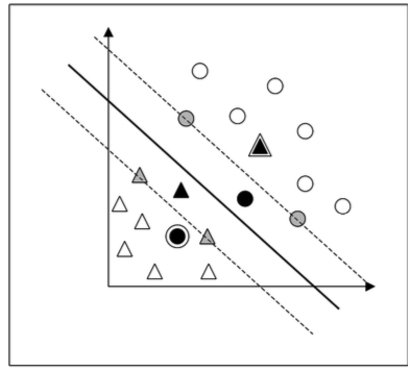
\includegraphics[width=0.4\linewidth]{figuras/margemSuave.pdf}
  \caption{Ilustração dos tipos de vetores de suporte: livres (cinza) e limitados (preto) \citeC{lorena2007}.}
  \label{fig:margemSuave}
\end{figure}

Em conclusão, obtém-se a mesma equação de classificação do modelo anterior (equação \ref{eq:eqSVM}), porém os parâmetros $a_i$ são calculados de forma distinta, com restrições que dependem da constante \textit{K}.

\subsubsection{SVM não-linear}

Apesar do modelo SVM com Margens Suaves ser mais abrangente do que aquele com Margens Rígidas, este modelo corresponde a um modelo de separação de categorias no qual um hiperplano é obtido, ou seja, é necessária uma característica linear na distribuição dos dados. No entanto, em aplicações reais, em alguns casos pode não ser possível seprar o subconjunto de dados por um hiperplano, como exemplificado na Figura \ref{fig:svmNL}.

\begin{figure}[H]
 \centering
  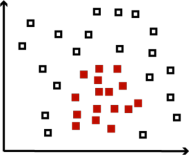
\includegraphics[width=0.35\linewidth]{figuras/svmNL.pdf}
  \caption{Ilustração de conjunto de dados de treinamento que não é linearmente separável}
  \label{fig:svmNL}
\end{figure}

Desta forma, atentando-se para a utilização da função \textit{kernel} (ver equação \ref{eq:eqSVM}), percebe-se que é possível empregar a SVM em uma classificação não linear, empregando um "truque de \textit{kernel}" { }(\textit{kernel trick}) que se resume em mapear os dados de entrada em um espaço com dimensão superior, denominado espaço de atributos (\textit{feature space}), como apresentado na Figura \ref{fig:svmKernel} \citeC{shawe2004} \citeC{boser1992}. Neste caso, observa-se $\phi:X\mapsto\eth$, no qual $\eth$ é o novo espaço de características. O bom desempenho do classificador depende de uma escolha apropriada de $\phi$, para que uma divisão linear nos dados de treinamento possa ser realizada.

\begin{figure}[H]
 \centering
  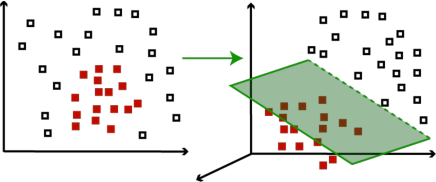
\includegraphics[width=0.75\linewidth]{figuras/svmKernel.pdf}
  \caption{Ilustração de mapeamento de conjunto de dados de treinamento em novo espaço de características a partir da utilização de função \textit{kernel}, possibilitando a divisão linear entre as categorias.}
  \label{fig:svmKernel}
\end{figure}

Segundo o teorema de Cover, para que os dados mapeados para o novo espaço de características tenham alta probabilidade de serem linearmente separáveis, duas condições devem ser satisfeitas \citeC{cover1965}. Primeiramente, a transformação ($\phi$) deve ser não-linear e, em segundo lugar, a dimensão do espaço de características deve ser suficientemente alta.

No processo de treinamento, ocorre o mapeamento dos dados de treinamento para o espaço de característicias aplicando-se $\phi$ no conjunto de dados. Com o objetivo de obter um nível relativamente baixo de ruídos, emprega-se a SVM com Margens Suaves. Após isso, as equações para otimização são calculadas, com a aplicação do operador $\phi$. Sendo assim, o classificador é o descrito na equação \ref{eq:eqSVM}.

Comumente, aplica-se o \textit{kernel} sem necessarimente a determinação prévia do operador $\phi$, deixando-o como uma operação implícita durante o treinamento. Esse é mais um motivo para usar a função \textit{kernel}, uma vez que se trata de um operador com cálculo simples (produto escalar) que representa bem os espaços. Para garantir que as condições expostas nesta seção sejam cumpridas, utilzam-se alguns tipos de \textit{kernel} que satisfazem as condições de Mercer \citeC{lorena2007}. As condições de Mercer são satisfeitas em um \textit{kernel} caso ele gere matrizes $\boldsymbol{K}$, em que cada elemento é definido por $K_{i,j}=K(\boldsymbol{x_i},\boldsymbol{y_j})$, para todo $i,j = 1,...,n$. Todos os \textit{kernels} que foram utilizados neste projeto são apresentados na Tabela \ref{tab:svmkernel}.

\begin{table}[h]
 \centering
 \begin{tabular}{l|c|c}
    Tipo & Função $k(x,x')$ & Parâmetros\\
  \hline
  Linear &  $(\delta(x \cdot x') + \kappa)$ & $\delta,\kappa$ \\
  Polinomial &  $(\delta(x \cdot x') + \kappa)^d$ & $\delta,\kappa, d$  \\
  RBF & $\exp(\frac{-||x - x'||^2}{2\sigma^2})$ & $\sigma$ \\
  Sigmoidal & $\tanh(\delta(x \cdot x') + \kappa)$ & $\delta,\kappa$ \\
 \end{tabular}
 \caption{Funções \textit{kernel} e seus parâmetros, utilizadas neste projeto \citeC{lorena2007} e \citeC{martin2012}}
 \label{tab:svmkernel}
\end{table}

\subsubsection{SVM Multiclasse}

Apesar de se tratar de um classficador que é intrinsicamente binário, a SVM pode também ser aplicada em problemas que apresentem várias categorias. Para tal, foram desenvolvidas ao longos dos anos novas soluções para a multiclassificação a partir de combinações múltiplas do classificador binário explicitado previamente nesta seção. Alguns modelos de adaptação do SVM para variadas classes são Um-contra-um (OvO, do inglês \textit{one vs. one}), Gráfico Acíclico Dirigido (DAG, do inglês \textit{Directed Acyclic Graph}), Código de Correção de Erro de Saída (ECOC, do inglês \textit{Error Corrected Output Coding}) e Um-contra-todos (OvA, do inglês \textit{One vs. All}), sendo este último utilizado neste projeto.


Supondo que um conjunto de dados possui $m$ classes, empregando a abordagem Um-contra-todos, um total de $m$ classificadores binários SVM devem ser criados para efetuar a classificação de uma determinada categoria em relação às $m-1$ demais classes. Então, no momento de testes ou de classificação de novos dados, esses dados são classificados criando-se uma margem (limiar de decisão) a partir do hiperplano separador e a classe desse dado será aquela que possuir uma função de decisão com maior valor, que corresponde à SVM que possui a maior margem dentre os demais \citeC{pal2008} \citeC{Bishop2006}.

Sendo assim, para um problema deste tipo, devem ser determinados $m$ hiperplanos. Consequentemente, é necessária a solução de $m$ problemas de otimização, sendo que, em cada um deles, uma classe é separada das demais. Desta forma, esta é uma desvantagem dessa abordagem, já que, durante a fase de treinamento, este processo é computacionalmente oneroso. Ademais, supondo que todas as classes possuam uma quantidade igual de amostras para treinamento, já que a SVM se comporta como um classificador binário, uma classe terá bem menos amostras para treino do que a outra classe, apresentando uma razão de $1:(m-1)$ \citeC{pal2008}.



\subsection{Floresta Aleatória}

O método Floresta Aleatória foi inicialmente proposto por Breiman \citeC{breiman2001} e pode ser aplicado tanto em problemas de classificação, quanto em problemas de regressão. O modelo classificador consiste em um conjunto de árvores aleatórias de decisão que são criadas durante o processo de treinamento do modelo, sendo escolhidos aleatoriamente os atributos dentro do vetor de entrada fornecido ao classificador \citeC{guedessistema}.

Passa-se, então, para o cálculo individual da entropia pertencente aos atributos. O atributo que apresenta a maior entropia é escolhido como sendo o nó que será utilizado na separação de classes nesta determinada posição na árvore. No caso deste modelo, o resultado final de classificação é obtido por meio da soma ponderada de predições sugeridas por diferentes conjuntos de parâmetros pertencentes às variadas árvores que compõem a floresta \citeC{prince2012}.

O método Floresta Aleatória possui várias vantagens, dentre elas \citeC{breiman2001}:

\begin{enumerate}
\item É um modelo relativamente robusto a ruídos;
\item É simples e é facilmente implementada de forma paralela;
\item Nas diversas aplicações na área, este método tem apresentado um melhor desempenho que outros em relação ao índice de acerto de classificação, métodos tais como a SVM e as Redes Neurais Artificias \citeC{caruana2008}.
\end{enumerate}

\subsubsection{Árvores de Decisão}

As árvores de decisão são uma técnica utilizada para a construção de modelos de classificação, que distribuiem os exemplos em um número finito de categorias. A técnica realiza a análise de um atributo, realizando a subdivisão dos dados do conjunto.

Sua estrutura se assemelha à uma árvore invertida, começando por um nó raiz e se subdividindo em ramos e em outros nós, até chegar em suas folhas, que são os pontos finais do sistema. Os nós internos são os nós de decisão e realizam o teste de atributos. Cada ramo está relacionado ao valor do atributo e, por último, cada folha representa uma classe \citeC{neto2014}.

Em geral, constroi-se uma árvore de decisão com um conjunto de dados de entrada, a partir do qual o nó raiz é criado e, após a realização de um teste, divide-se a árvore em ramos. Esse processo de avaliação do nó e da divisão em ramos é realizado nos nós subsequentes também, continuando a ramificação da árvore. Esse processo é realizado até que se atinja uma folha, não havendo mais ramificação. Todo esse procedimento é realizado recursivamente para conjunto de dados \citeC{bosch2007}.

\subsubsection{Procedimento da Floresta Aleatória}

A técnica de Floresta Aleatória é composta por um conjunto de árvores de decisão, no processo de crescimento de cada árvore é usado algum tipo de técnica aleatória. O conjunto de dados completo é dividido em subconjuntos, que serão os dados iniciais fornecidos à cada árvore. A aleatoriedade pode ser empregada durante o processo de divisão do conjunto de dados e na seleção do teste de cada nó.

No algoritmo de Floresta Aleatória, as árvores são binárias e os testes para decisão em cada nó podem ser escolhidos de forma aleatória, independentemente dos dados, ou por meio de um algoritmo que escolhe o teste que separa de melhor forma as amostras de treinamento. Neste caso, faz-se uma avaliação de acordo com a seguinte equação

\begin{equation}
\label{eq:randomF}
 \Delta E =
 - \displaystyle\sum_{i}\frac{|Q_i|}{|Q|}E(Q_i)
\end{equation}

na qual $\Delta E$ é o ganho de informação, que é gerado quando um conjunto de dados $Q$ é dividido em subconjuntos $Q_i$.

$E(q)$ é a entropia apresentada na seguinte expressão

\begin{equation}
\label{eq:entropy}
 E(q) = - \displaystyle\sum_{j=1}^{N}p_jlog_2(p_j)
\end{equation}

na qual $p_j$ é a proporção dos exemplos em $q$ que pertencem à classe $j$. Todo esse processo é recursivo e seu critério de parada pode ser pré-determinado escolhendo-se a quantidade de estimadores que serão utilizados na floresta, como no caso deste projeto. Outro critério de parada que pode ser utilizado é avaliar quando um nó não recebe exemplos suficientes.

Neste classificador, utiliza-se o conceito de probabilidade a posteriori, que se trata de probabilidade condicional de determinado evento aleatório. Durante o processo de treinamento do modelo, a probabilidade a posteriori é calculada para cada classe $c$ em cada folha $l$, que pertence à determinada árvore $a$. Essa probabilidade pode ser calculada como mostra a seguinte equação

\begin{equation}
\label{eq:probabilidade}
 P_{a,l}(Y(I)=c) = \frac{N_{c,l}}{N_l}
\end{equation}

 sendo que $Y(I)$ é a classe $c$ de determinanda imagem $I$, $N_{c,l}$ é o número de imagens da classe $c$ que chegaram à folha $l$ e, por último, $N_l$ é o número do total de imagens que alcançaram a folha $l$ \citeC{bosch2007}.

O processo de treinamento, avaliando as imagens do conjunto de treinamento, é inicializado no nó raiz e, então, passa pelas árvores de decisão até atingir alguma folha. Sendo assim, a classe daquela imagem é definida tomando-se o argumento máximo da média artimética de todas as probabilidades a posteriori.

No capítulo seguinte, retrata-se a metodologia utilizada no desenvolvimento deste projeto, relatando os processos de composição do banco de imagens, bem como os estágios de pré-processamento, extração de atributos e de treinamento utilizando-se os classificadores descritos no presente capítulo.
% breiman2001
%The common element in all of these procedures is that for the kth tree, a random vector  k is generated, independent of the past random vectors  1,..., k−1 but with the same distribution; and a tree is grown using the training set and  k, resulting in a classifier h(x, k) where x is an input vector.

%For instance, in bagging the random vector   is  generated as the counts in N boxes resulting from N darts thrown at random at the boxes, where N is number of examples in the training set. In random split selection   consists of a number of independent random integers between 1 and K . The nature and dimensionality of   depends on its use in tree construction.
%After a large number of trees is generated, they vote for the most popular class. We call these procedures random forests.

%Definition 1.1. A random forest is a classifier consisting of a collection of tree-structured classifiers {h(x,  k ), k = 1, . . .} where the { k } are independent identically distributed random vectors and each tree casts a unit vote for the most popular class at input x.

%To improve accuracy, the randomness injected has to minimize the correlation ρ ̄ while maintaining strength. The forests studied here consist of using randomly selected inputs or combinations of inputs at each node to grow each tree.

%Advantages

%ii It’s relatively robust to outliers and noise.
%iii It’s faster than bagging or boosting.
%iv It gives useful internal estimates of error, strength, correlation and variable importance.
%v It’s simple and easily parallelized.

%SEÇAO 10 = MECANISMO
%FALAR SOBRE CART TBM (livro)







\chapter{Metodologia}
\label{ch:Metodologia}

Neste capítulo são descritas as etapas de desenvolvimento do projeto que já foram implementadas, tendo em vista a proposta apresentada para construção de um produto de tecnologia assistiva para ensino de tipografia a deficientes visuais, mais especificamente, do sistema de classificação de tipografias.

O processo de desenvolvimento do sistema se deu em três etapas principais, que são listadas a seguir:

\begin{enumerate}
\item Estruturação do projeto;
\item Composição do banco de dados (imagens das diversas tipografias);
\item Implementação do algoritmo para classificação das imagens.
\end{enumerate}
%\ldots - reticencias

A primeira etapa deste trabalho foi caracterizada por debates para a idealização do produto final de tecnologia assistiva oferecido ao deficiente visual. A segunda e a terceira etapas, por sua vez, foram desenvolvidas e aprimoradas simultaneamente. O processo de desenvolvimento adotado nessas etapas é explicitado abaixo.

Todos os algoritmos implementados para este projeto, bem como o banco de imagens, podem ser encontrados no \textit{link}: \textit{github.com/fegvilela/TCC2}.

%Os resultados dessa etapa foram descritos no capítulo 2, como fundamentação teórica, e no capítulo 1, como apresentação da proposta de projeto. Porém, tópicos em relação ao projeto final do produto encontram-se na seção destinada a trabalhos futuros.
\section{Estruturação do Projeto}

Como primeiro estágio de desenvolvimento do projeto, foram discutidos modelos para a estruturação do produto e realizadas pequenas entrevistas não-estruturadas com deficientes visuais, sendo eles possíveis usuários do produto ou não.

Em oportunidades de teste, descritos e implementados no trabalho de Cruz \citeC{cruz2017}, para aperfeiçoamento das peças táteis no desenvolvimento do produto, também foram realizadas as entrevistas com os deficientes visuais. O foco dessas entrevistas foi o maior entendimento sobre o contato real dos deficientes com o computador e com a informática. Nestas ocasiões, foram questionados aspectos sobre os leitores de tela disponíveis no contexto brasileiro, além de a popularização do sistema operacional \textit{DOSVOX}. O objetivo dessas questões foi direcionar o desenvolvimento futuro do sistema, para que ele seja adaptado às condições reais de tecnologia dos deficientes visuais brasileiros. Além disso, houve a apresentação da proposta do sistema, a qual foi avaliada positivamente.

Vale ressaltar que o contato realizado com estes deficientes visuais foi importante para a idealização e desenvolvimento do projeto até o momento, sendo um vínculo importante para o seguimento deste posteriormente.

\section{Composição do Banco de Imagens}

Passando-se então para as etapas de implementação do sistema, como já descrito, foram escolhidas nove tipografias para o projeto e, para cada uma delas, construído um conjunto de imagens. Para melhor organização, o banco foi montado tipografia a tipografia. As imagens que compõem o banco de dados em sua versão final são caracteres separados de cada tipografia, amostras podem ser vistas na Figura \ref{fig:nimage}.


A principal fonte de obtenção das imagens originais foi o \textit{Fonts in Use}, um website que disponibiliza fotografias de projetos envolvendo design gráfico que já estão classificadas por tipografia \citeC{fontsinuse2017}. Além deste, foram utilizados sites de busca convencionais, utilizando a opção de imagens nas buscas. Ainda, para os casos em que poucas imagens foram encontradas, a saber as tipografias \textit{Franklin Gothic} e \textit{Adobe Jenson}, imagens complementares foram cedidas como cortesia pela estudante de design parceira neste projeto.


\begin{figure}[H]
  \centering
  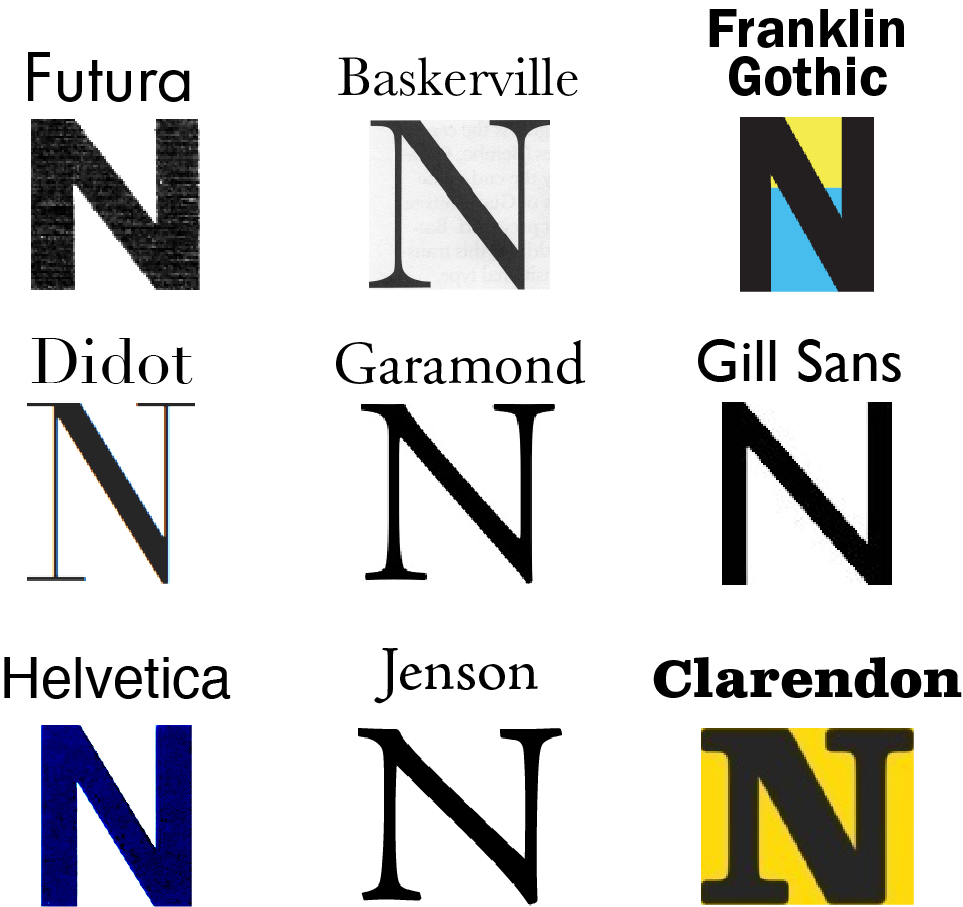
\includegraphics[width=0.4\linewidth]{figuras/nimage.pdf}
  \caption{Amostras do banco de imagens, especificando-se a tipografia.}
  \label{fig:nimage}
\end{figure}


É comum que tipografias digitais apresentem várias versões distintas entre si. Uma vez que as tipografias digitais são representações da versão física original dos tipos, diversas fundidoras de tipos propõem seu próprio modelo representativo para aquela tipografia, ocasionando em variações nas versões digitais. Um exemplo utilizando a tipografia \textit{Garamond} é apresentado na Figura \ref{fig:comparacaoTipos}. Escolheu-se, para ilustração, a letra "a", sendo possível verificar as diferenças no formato de três partes específicas da letra: bojo, remate e terminal em gota. A versão adotada no projeto é a \textit{Adobe Garamond Pro}. Logo, antes de adquirirmos imaens deste tipo em websites, foi necessária uma análise manual para verificar se a imagem se tratava da tipografia correta, em sua versão empregada no projeto.


\begin{figure}[h!]
  \centering
  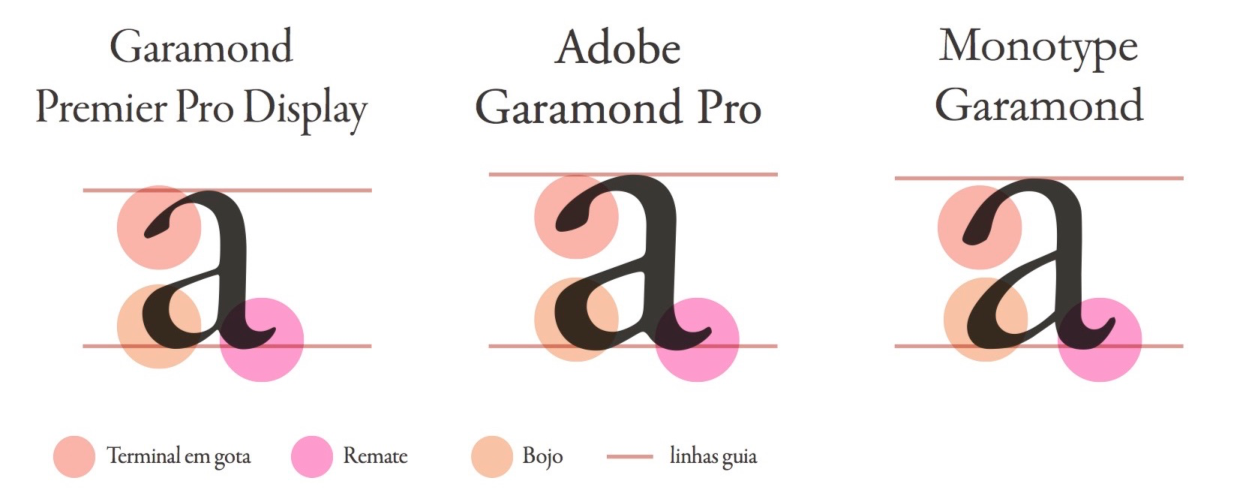
\includegraphics[width=0.65\linewidth]{figuras/comparacaoTipo.pdf}
  \caption{Comparação entre três versões da fonte Garamond, evidenciando as partes anatômicas distintas.}
  \label{fig:comparacaoTipos}
\end{figure}

Sendo assim, a adição de uma imagem de uma outra versão da tipografia poderia gerar um erro de classificação, já que algumas tipografias empregadas no projeto são similares entre si, fato ilustrado na Figura \ref{fig:comparacaoJensonGaramond} que apresenta a similaridade entre duas tipografias presentes no projeto. Portanto, a análise foi realizada de forma minuciosa, utilizando conceitos da anatomia das letras, como o formato de suas serifas e o contraste entre as partes \citeC{rocha2004}. Ademais, as imagens originais obtidas muitas vezes continham variações que deveriam ser excluídas manualmente, como mais de uma tipografia em sua composição, ou então uma mistura entre os variados estilos dentro de uma família tipográfica: itálico, algumas variações de negrito e versalete.

\begin{figure}[H]
  \centering
  
\includegraphics[width=0.4\linewidth]{figuras/comparacaoJensonGaramond.pdf}
  \caption{Comparação entre as fontes \textit{Adobe Garamond Pro} e \textit{Adobe Jenson Pro}, atestando o alto índice de similaridade entre elas.}
  \label{fig:comparacaoJensonGaramond}
\end{figure}

Para o processo de separação das imagens em caracteres únicos, implementou-se um algoritmo em Python para automatização do processo de reconhecimento da localização dos caracteres na imagem e de formação de novas imagens individuais, algo similar a "recortes" {} da imagem original. A principal biblioteca utilizada nesse algoritmo foi a \textit{OpenCV} (\textit{Open Source Computer Vision Library}), uma biblioteca de visão computacional e aprendizado de máquina disponível em código livre (\textit{open source}). Ela foi escolhida por ser amplamente utilizada por especialistas da área e em empresas renomadas como Google, Microsoft, Intel e IBM \citeC{opencv2017}.

O algoritmo desenvolvido é composto de uma seção principal denominada \texttt{mainBancoDados}, e de módulos importados, que incluem os métodos (estruturas em Python análogas à funções) implementados para desempenhar operações específicas nas imagens. O fluxograma do código é ilustrado na Figura \ref{fig:flowMain}. Ao executar o algoritmo, deve-se escolher em qual parte do banco de dados, ou seja, qual tipografia, deseja-se analisar. A seção principal dá acesso à execução de três operações (métodos implementados nesse projeto): recorte das imagens originais, exclusão das imagens de dimensão pequena e renomeação das imagens.

Inicia-se com a aplicação da operação de recorte de imagens (o método \texttt{imCrop}) caso as imagens não sejam letras individuais. Então, caso haja erro no reconhecimento das letras, sendo formada alguma imagem que não apresenta um único caractere por completo, passa-se para o método de exclusão de imagens (\texttt{imApaga}). Em seguida, utilizando o método \texttt{changeName}, realiza-se a renomeação das imagens, caso elas não possuam o nome adequado.

 Vale ressaltar que a formatação padrão para o nome das imagens foi escolhida como: \textit{numero\_tipografia}. Por exemplo, o nome da sétima imagem presente no diretório da tipografia \textit{Helvetica} será "7\_helvetica". O caractere "\_" {} foi escolhido nesse caso para que a classe da imagem, a tipografia, seja de fácil identificação pelo algoritmo de treinamento do modelo classificador.


\begin{figure}[h!]
  \centering
  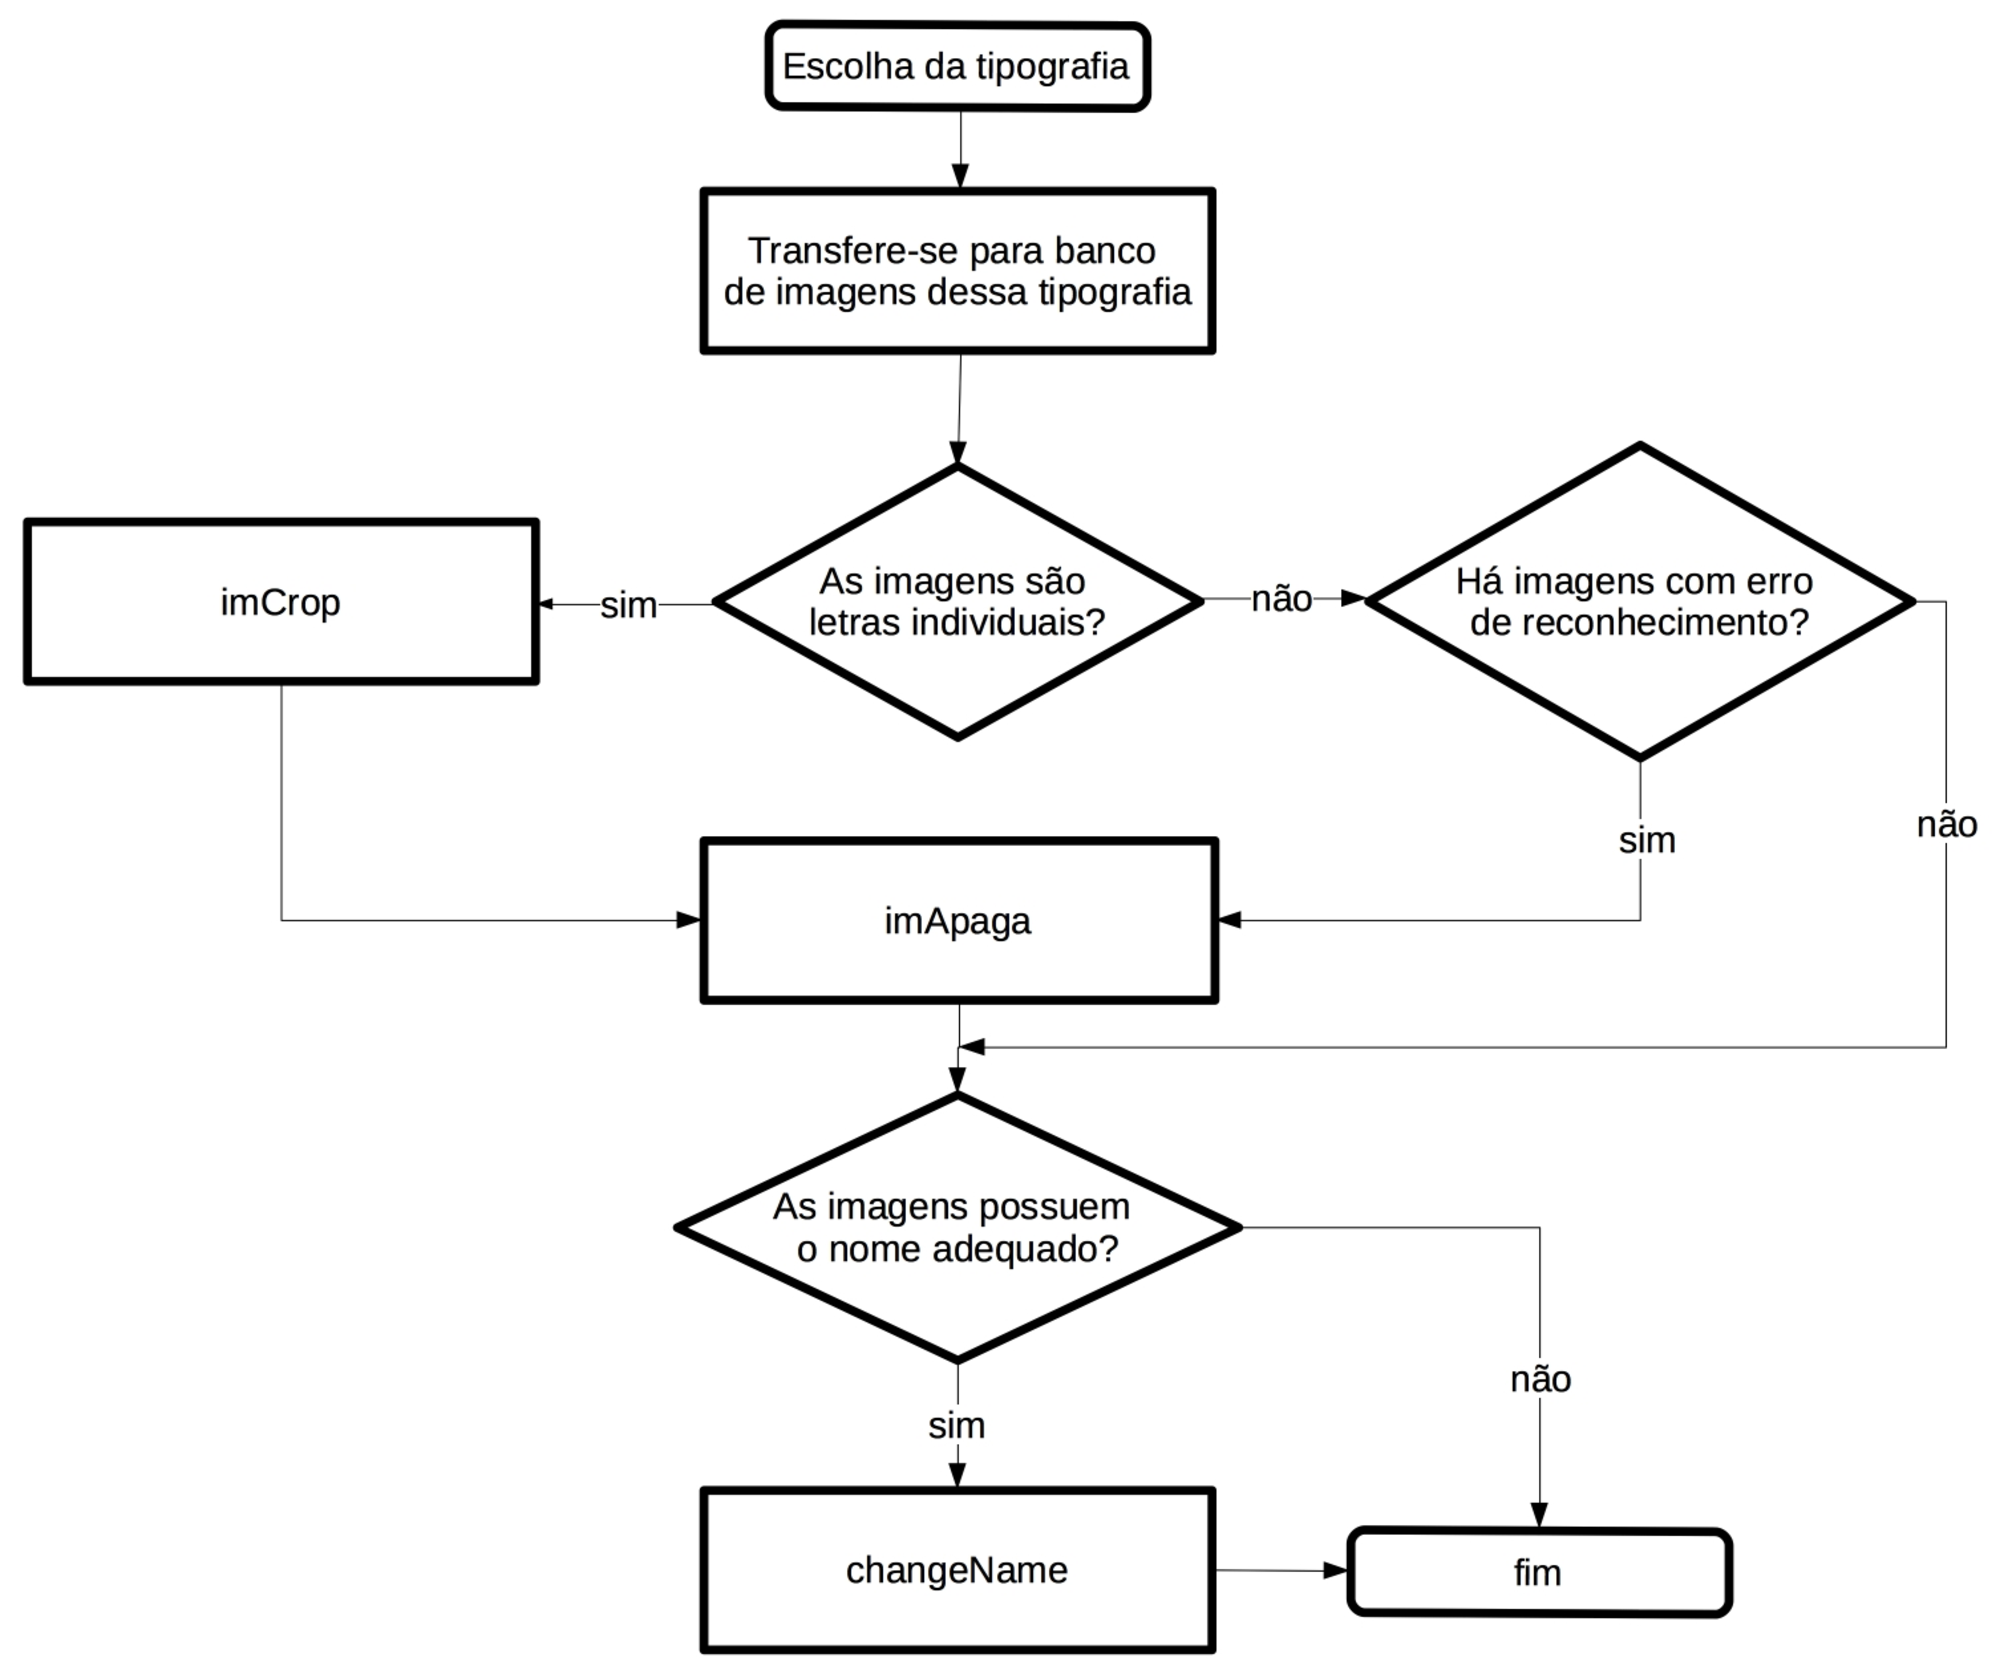
\includegraphics[width=0.9\linewidth]{figuras/mainbancodados.pdf}
  \caption{Fluxograma da seção principal do algoritmo para composição do banco de dados}
  \label{fig:flowMain}
\end{figure}

Passa-se, então, para a descrição de cada um desses métodos separadamente. Em primeiro lugar, o método \texttt{imCrop} realiza o recorte das imagens originais, criando imagens individuais de caracteres. O fluxograma está apresentado na Figura \ref{fig:flowimCrop}. Quando chamado na seção principal, o método \texttt{imCrop} recebe como parâmetro de entrada o nome da fonte em que se deseja operar, já que o banco de imagens é dividido por tipografias. Então, o diretório de operação passa a ser o banco de imagens da fonte escolhida. Todas as imagens contidas naquele diretório são convertidas para o formato \textit{PNG}, que é um dos formatos aceitos pela biblioteca \textit{OpenCV}.


\begin{figure}[H]
  \centering
  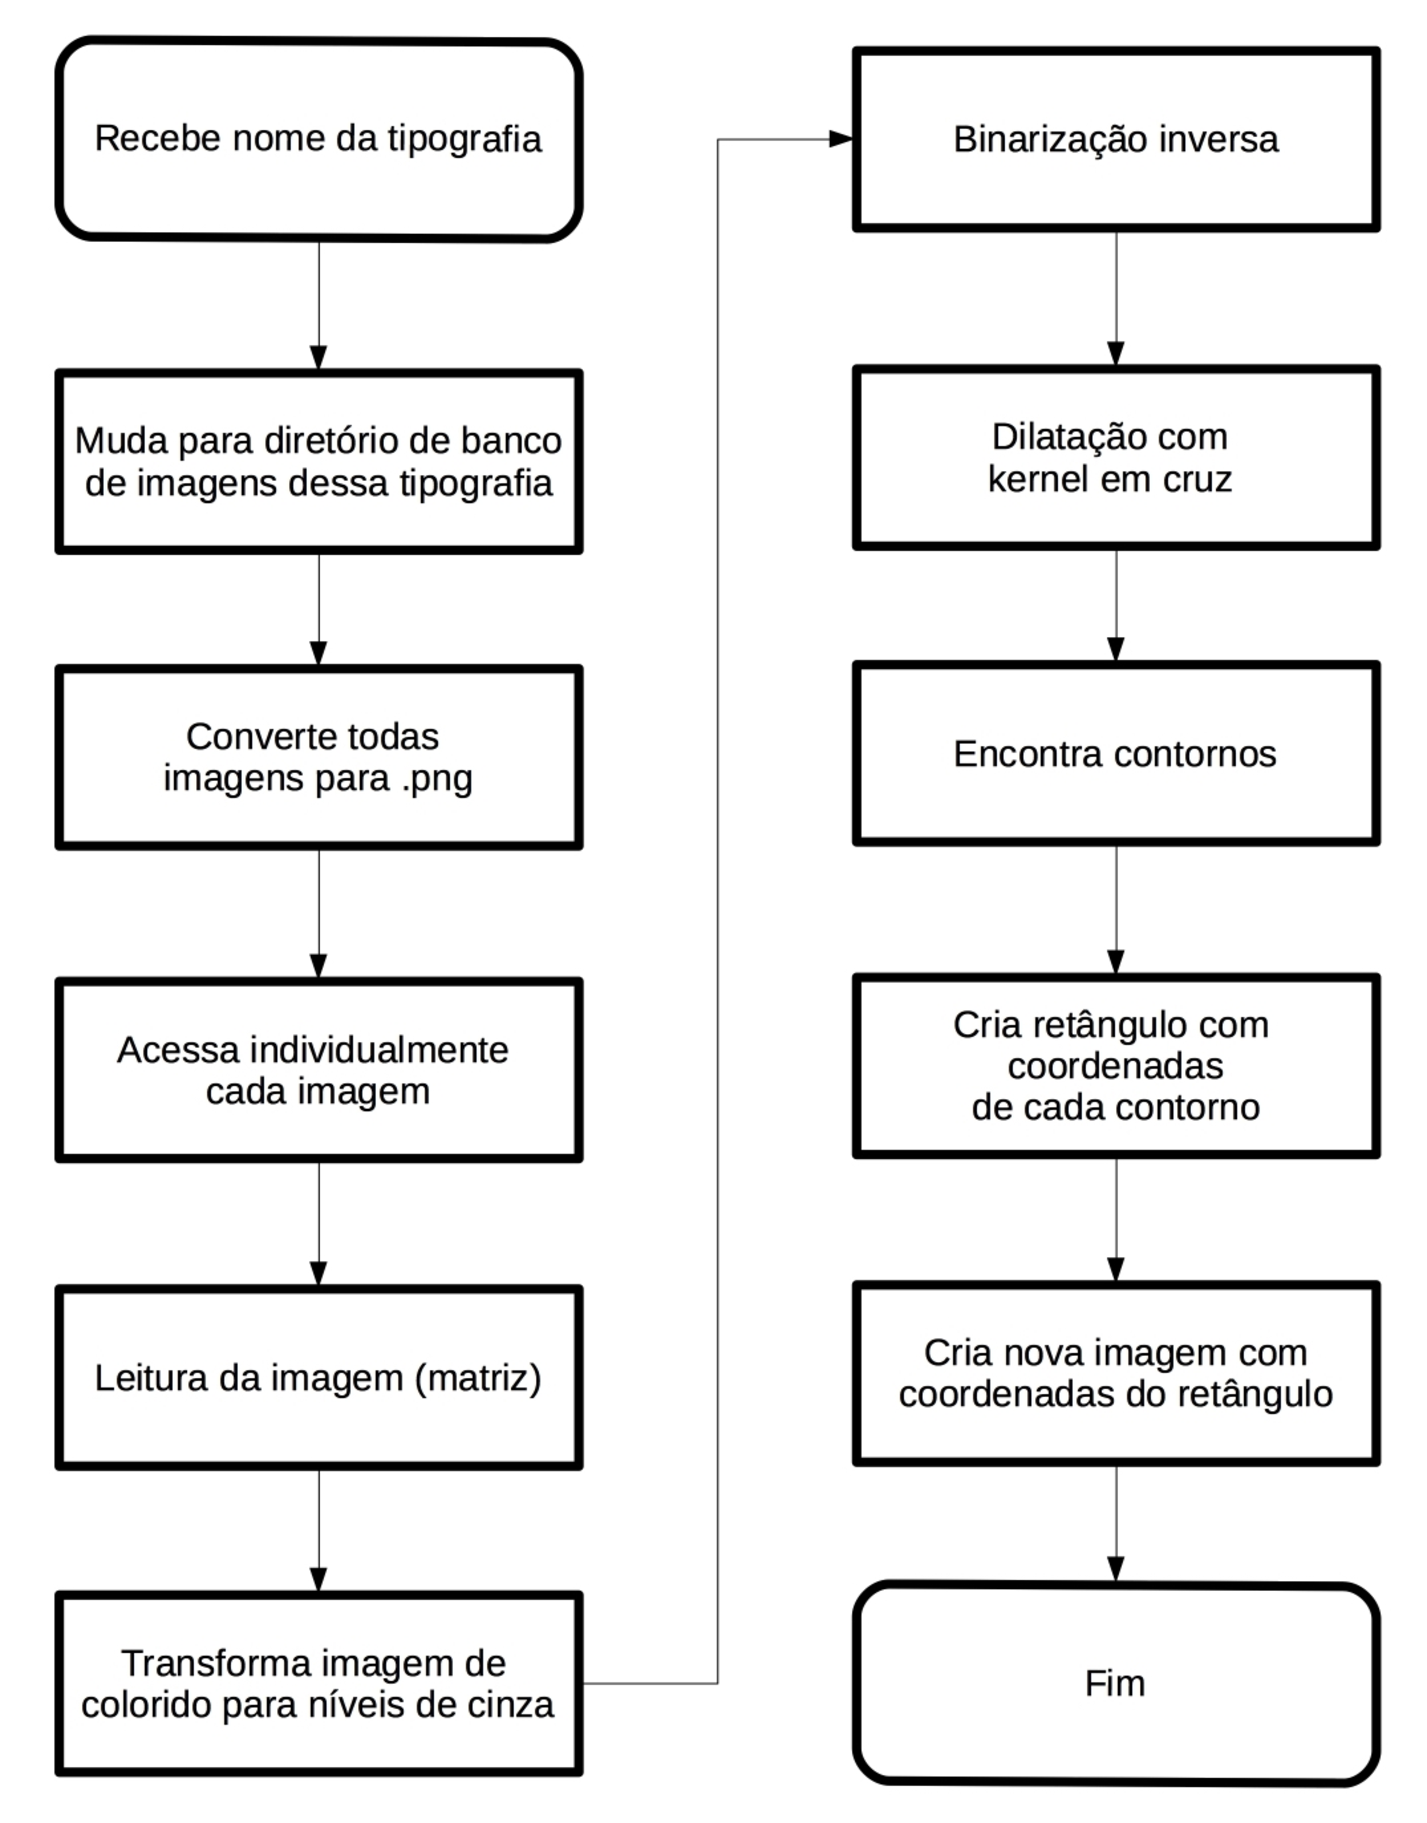
\includegraphics[width=0.6\linewidth]{figuras/imCrop.pdf}
  \caption{Fluxograma do método \texttt{imCrop} para recortar as imagens originais, criando imagens separadas de cada caractere.}
  \label{fig:flowimCrop}
\end{figure}

As imagens são acessadas individualmente e lidas uma por vez. Os valores dos pixels de uma imagem são armazenados em uma matriz. A imagem colorida é convertida para níveis de cinza e, em seguida, é realizada a binarização inversa da imagem em tons de cinza, utilizando um limiar de nível 88, ou seja, valores acima de 88 são atribuídos como valor zero (preto) e valores abaixo, como valor unitário (branco). O próximo passo é a dilatação morfológica usando um \textit{kernel} em cruz, com dimensão 3x3. Após isso, encontram-se os contornos de cada parte branca da imagem. São criados retângulos limitadores ao redor dessas partes da imagem, utilizando as coordenadas dos contornos e novas imagens são criadas a partir desses retângulos. Todo o processo é exemplificado na Figura \ref{fig:imProcess} para uma imagem da fonte \textit{Futura}.



Vale ressaltar que, por envolver um processo de binarização inversa no algoritmo, não foi possível efetuar a detecção de borda nas letras das imagens que, em escala de cinza, possuíam cor de fundo com tom mais escuro que aquele da letra. Portanto, se fez necessária uma correção na coloração de algumas imagens para melhor desempenho do algoritmo, processo realizado manualmente, no software \textit{Pré-Visualização} do sistema operacional \textit{Mac OS X} e também no software \textit{Adobe Lightroom}. Além disso, em algumas imagens, as letras em texto encontravam-se muito próximas uma à outra, o que gerou a demanda de uma limpeza de partes residuais de outras letras, após a formação das imagens de caracteres individuais.

\begin{figure}[H]
  \centering
  
\includegraphics[width=0.9\linewidth]{figuras/imProcess2.pdf}
  \caption{Resultado por etapa do processo de reconhecimento de caracteres em imagens do banco de imagens. i)imagem original, ii)escala de cinza, iii)binarização inversa, iv)dilatação com \textit{kernel} em cruz e v)contornos e retângulos limitadores}
  \label{fig:imProcess}
\end{figure}

O próximo método utilizado na seção principal do algoritmo é \texttt{imApaga}, responsável por excluir as imagens que possuem ambas dimensões inferiores a 45 pixels. O fluxograma descritivo pode ser visto na Figura \ref{fig:flowimApaga}.


\begin{figure}[H]
  \centering
  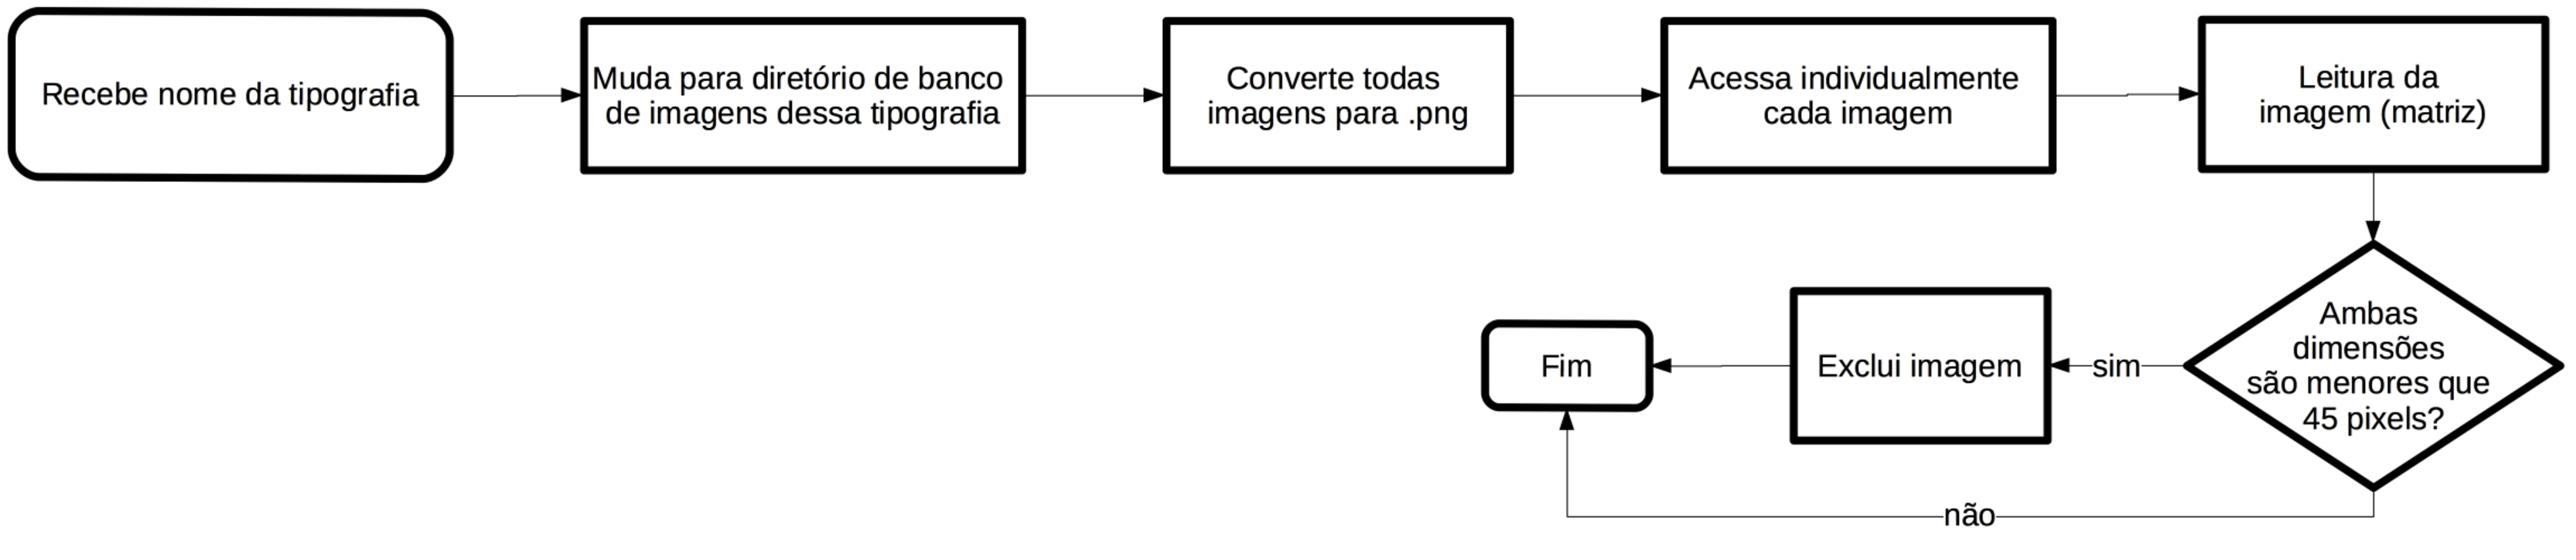
\includegraphics[width=1\linewidth]{figuras/imApaga.pdf}
  \caption{Fluxograma do método \texttt{imApaga} para excluir imagens com dimensões pequenas}
  \label{fig:flowimApaga}
\end{figure}

Assim como no método \texttt{imCrop}, recebe-se como parâmetro de entrada o nome da tipografia em que se deseja operar e muda-se para o diretório do banco de imagens da tipografia. Faz-se também a conversão de todas imagens para \textit{PNG}, que são depois acessadas individualmente e lidas, armazenando as intensidades dos pixels em uma matriz. Após isso, as dimensões da imagem são reconhecidas e avaliadas. Caso as duas dimensões sejam menores que 45 pixels, a imagem é excluída. Caso contrário, o programa passa para a próxima imagem, até finalizar a análise de todas as imagens presentes naquele diretório.

Por sua vez, o método \texttt{changeName} é utilizado para renomear as imagens presentes no diretório de acordo com a tipografia a que pertencem, seguindo o padrão estabelecido para o projeto (\textit{numero\_tipografia}). O fluxograma desse método é apresentado na Figura \ref{fig:flowchangeName}. Assim como os demais métodos dessa seção, começa-se recebendo o nome da tipografia em qual se deseja operar e transfere-se para o diretório do banco de imagens dessa tipografia.

A biblioteca (\textit{OS}) em \textit{Python} utilizada nesse método para a renomeação de arquivos pode gerar um problema durante o processo. Caso o novo nome escolhido para renomear um arquivo seja pertencente a um outro arquivo já existente no diretório, este arquivo prévio é excluído. Portanto, para evitar que arquivos sejam excluídos erroneamente apenas por receberem nomes repetidos, primeiramente verifica-se se há o caractere "\_" {} no nome dos arquivos. Caso negativo, utiliza-se a nomenclatura padrão supracitada, pois, dessa forma, não existirá arquivos prévios com nomenclatura semelhante a essa (\textit{numero\_tipografia}). Porém, caso a verificação apresente resultado positivo, nomeiam-se todos os arquivos com nomenclatura sem o caractere "\_" {}. Esse processo é realizado para garantir que, naquele diretório, nenhuma imagem possui a nomenclatura padrão, prevenindo-a de ser excluída. Então, posteriormente, utiliza-se a nomenclatura padrão em segundo processo automático de renomeação.


O banco de imagens, em versão final, constitui-se de 6750 imagens no total, sendo 750 imagens por tipografia, com dimensão mínima de 45 pixels em altura ou largura. No entanto, inicialmente, para as primeiras quatro tipografias, o banco contava com 1895 imagens para cada uma delas. Porém, muitas imagens possuiam dimensão pequena, apresentando baixa resolução e ruídos, fato que comprometia o treinamento e, consequentemente, a acurácia do classificador. Sendo assim, decidiu-se reduzir o tamanho do banco de imagens, exluindo automaticamente aquelas que fossem menor do que a dimensão desejada. Além disso, em alguns casos, aprouve-se operar uma exclusão manual de imagens provenientes de erros de reconhecimento realizado pelo algoritmo ou que apresentavam baixa resolução, apesar de dimensão maior do que 45 pixels.


\begin{figure}[H]
  \centering
  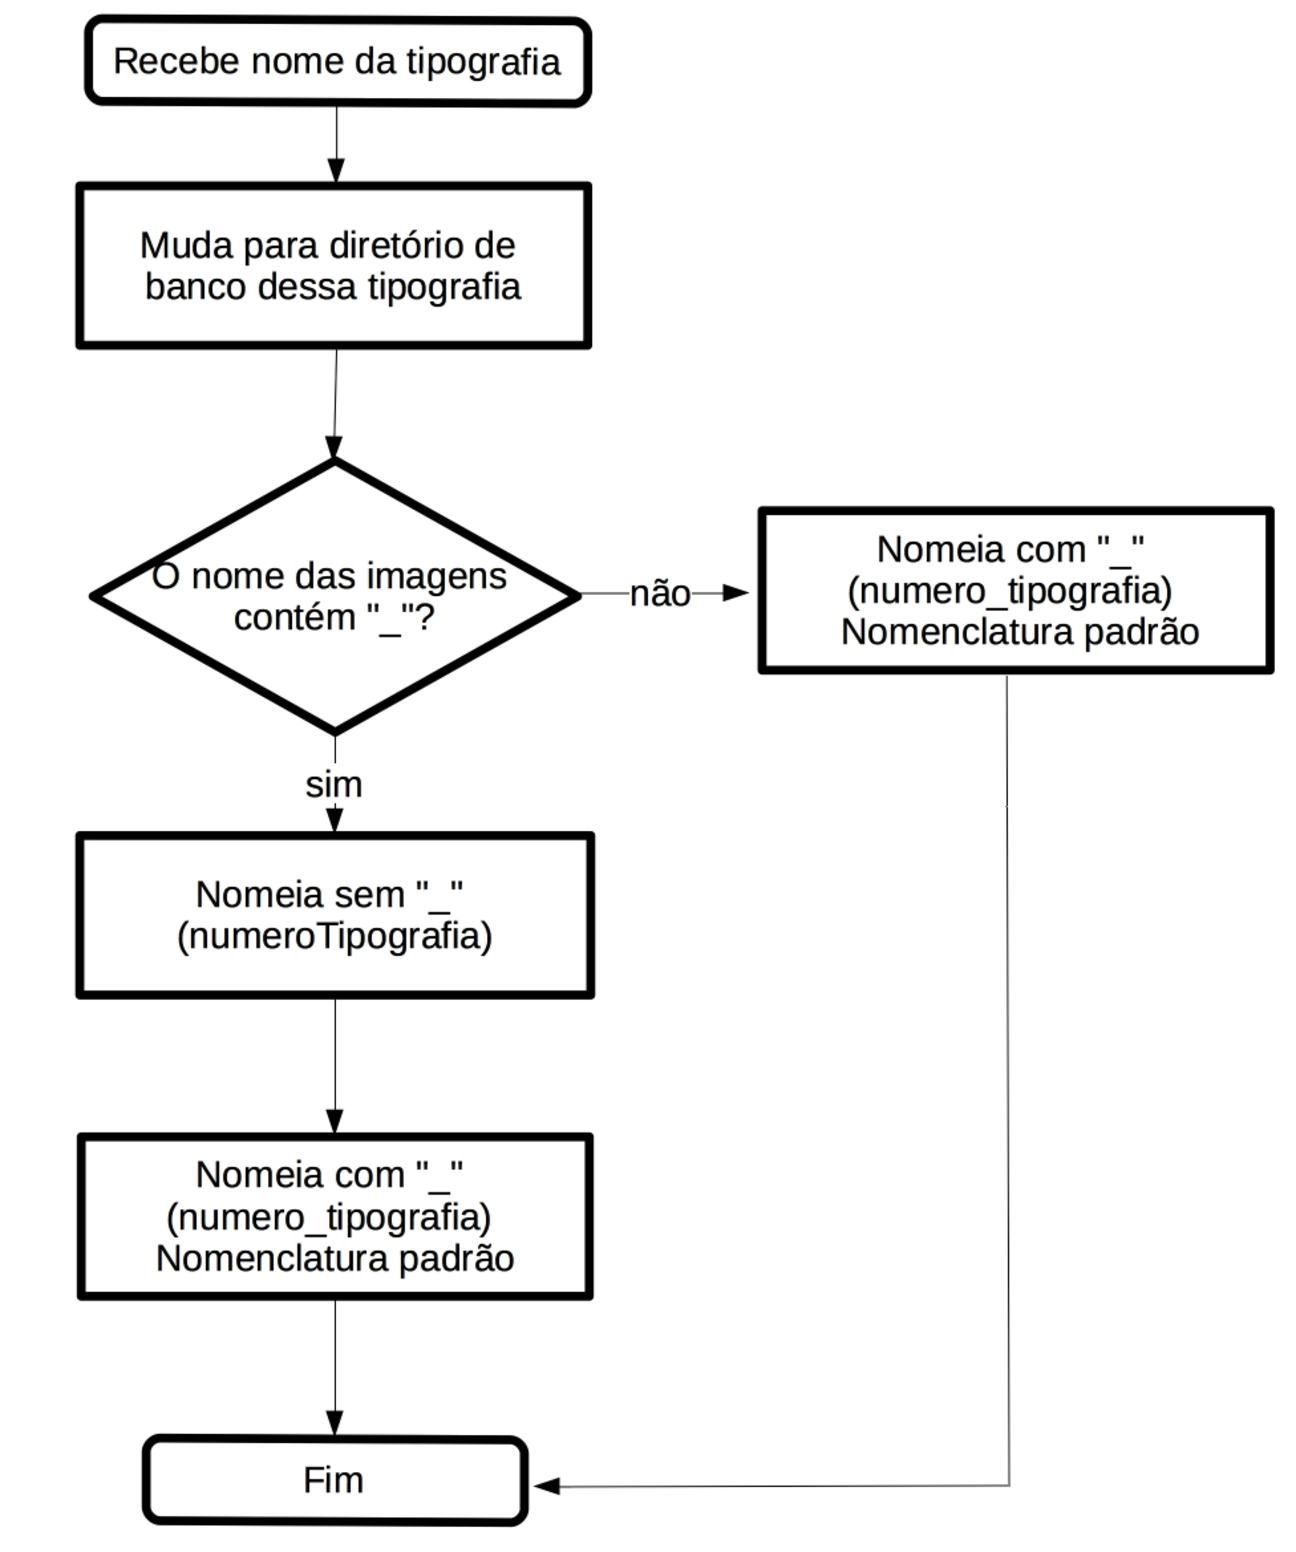
\includegraphics[width=0.55\linewidth]{figuras/changeName.pdf}
  \caption{Fluxograma do método \texttt{changeName} para renomear imagens de determinado diretório, preparando-as para o treinamento do modelo.}
  \label{fig:flowchangeName}
\end{figure}

%O processo de composição do banco de imagens para o treinamento do modelo a ser empregado na máquina foi a parte que mais demandou tempo em todo o processo de desenvolvimento do software. No entanto, em projetos nos quais a aprendizagem de máquina é utilizada essa etapa costuma ser descrita como demorada, como por exemplo (referência).


\section{Algoritmo para Treinamento do Modelo}

Essa seção destina-se à descrição do algoritmo implementado para treinamento do modelo da máquina, bem como das ferramentas utilizadas para seu desenvolvimento. O algoritmo é composto de três estágios listados a seguir, sendo que o resultado de um é o dado de entrada para o estágio subsequente:

\begin{enumerate}
\item Pré-processamento;
\item Extração de atributos;
\item Treinamento do modelo classificador e testes de predição.
\end{enumerate}

Vale ressaltar que as etapas de pré-processamento e de extração de atributos são consecutivas e feitas imagem a imagem, até que todas as imagens do banco sejam avaliadas. Sendo assim, uma imagem passa pelo estágio de pré-processamento, em seguida, pelo estágio de extração de atributos, para que, então, siga-se para a próxima imagem, realizando o mesmo processo.

O algoritmo foi também implementado em Python utilizando como bibliotecas principais o \textit{SciKit-learn}, o \textit{SciKit-image}, o \textit{NumPy} e o \textit{OpenCV}. Todas as bibliotecas citadas, exceto a \textit{OpenCV}, são derivadas de uma só coleção de bibliotecas, denominada \textit{SciPy}, que apresenta softwares de código livre para computação científica em Python. No entanto, as bibliotecas \textit{SciKit}, abreviação de \textit{SciPy Toolkits}, são pacotes complementares ao \textit{SciPy}, sendo desenvolvidas independentemente. O motivo de escolha dessas bibliotecas foi que eles são amplamente utilizados na área de processamento de imagens e aprendizado de máquina \citeC{skimage2014}  \citeC{sklearn2011} \citeC{scipy2017} \citeC{numpy2017}.

\subsection{Estágio de pré-processamento}

Para essa etapa, a principal biblioteca utilizada foi o  \textit{OpenCV}, com a qual foi implementado um processo similar ao método \texttt{imCrop} descrito na seção anterior. Todos os passos do pré-processamento encontram-se ilustrados na Figura \ref{fig:flowpreProc}.

\begin{figure}[h!]
  \centering
  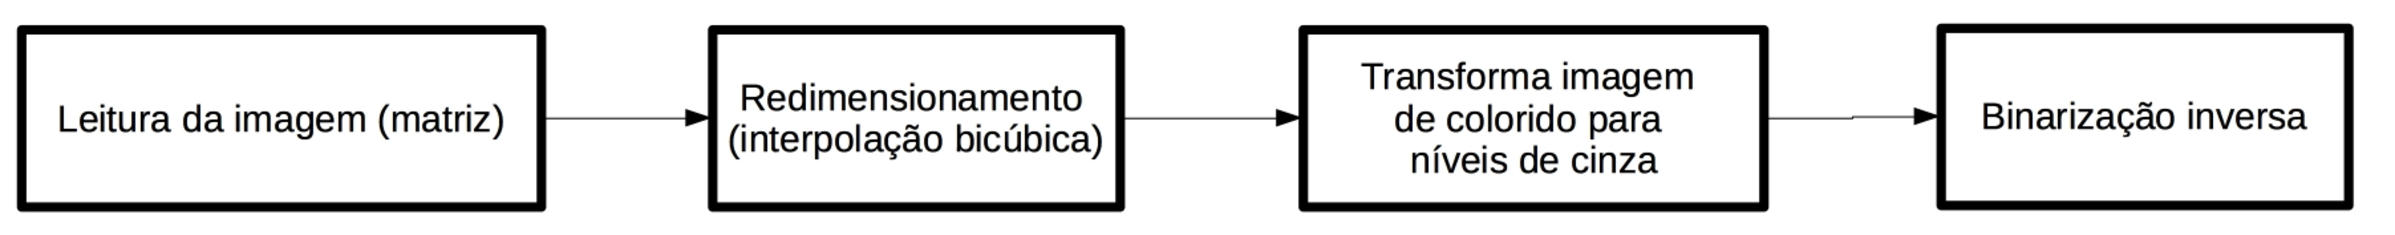
\includegraphics[width=1\linewidth]{figuras/preprocess.pdf}
  \caption{Etapas do estágio de pré-processamento do algoritmo de treinamento do modelo.}
  \label{fig:flowpreProc}
\end{figure}

Inicia-se pela leitura da imagem, transformando-a em matriz, seguido de seu redimensionamento por interpolação bicúbica para altura fixa de 126 pixels, garantindo, assim, uma melhor uniformidade das imagens para o processo de extração de atributos. O valor ótimo da nova dimensão foi encontrado por meio de iterações e testes de acurácia. Para esse teste, criou-se um \textit{loop} para alterar o valor da nova dimensão das imagens e, para cada valor de dimensão, o modelo era treinado e avaliada a acurácia. Desta forma, escolheu-se a dimensão que proporcionou maior acurácia. Posteriormente, a imagem é convertida para escalas de cinza e, por fim, é realizada uma binarização inversa da imagem.

 %Todo esse processo é demonstrado como exemplo na Figura X.

%\begin{figure}[H]
%  \centering
%  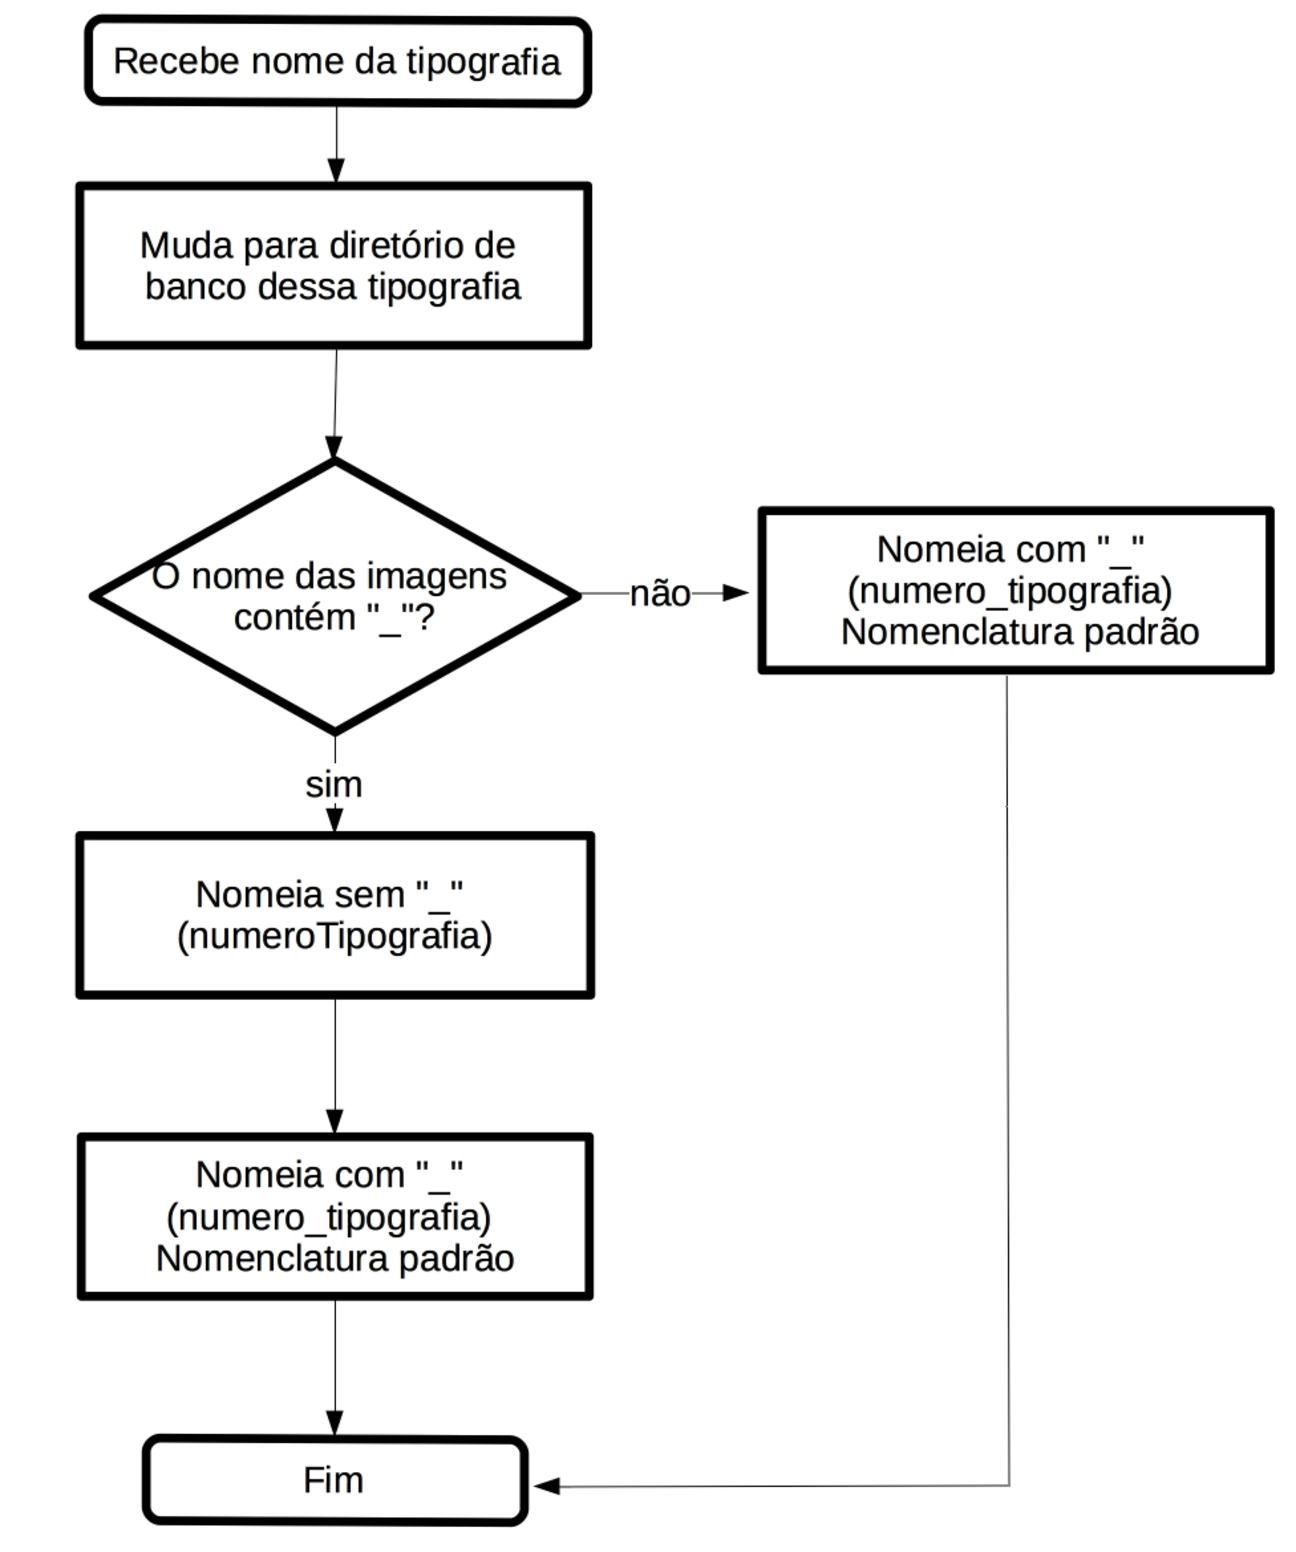
\includegraphics[width=0.6\linewidth]{figuras/changeName.pdf}
%  \caption{Fluxograma do método \texttt{changeName} para renomear imagens de determinado diretório, preparando-as para o treinamento do modelo - \textbf{Fonte:} Autora}
%  \label{fig:flowpreProc}
%\end{figure}

\subsection{Estágio de extração de atributos}

No estágio de extração de atributos, as bibliotecas usadas foram \textit{NumPy} e \textit{SciKit-image}. A biblioteca \textit{NumPy} é diretamente associada ao \textit{SciPy} e uma de suas vantagens principais é oferecer grande praticidade ao empregar matrizes, principalmente com uma vasta quantidade de elementos, por isso é utilizada em aplicações com imagens, como no caso deste projeto.

Dessa mesma forma, a biblioteca \textit{SciKit-image} foi utilizada no algoritmo por ser uma biblioteca desenvolvida para processamento de imagem. Apenas um módulo da biblioteca, a saber \texttt{feature}, foi utilizado para implementar a extração de atributos por meio do \textit{Local Binary Pattern} (LBP).

A seção de extração de atributos das imagens foi implementada como uma classe nomeada \texttt{LocalBinaryPattern}, em um módulo separado, e o modelo utilizado foi o LBP. Os parâmetros necessários para a sua aplicação na imagem, como explicado no capítulo \ref{ch:ML}, são: o raio (R) e a quantidade de pontos avaliados (P).

Sendo assim, esses valores devem ser fornecidos ao se utilizar a classe na seção principal do algoritmo. Os valores adotados nesse caso foram um raio de 9 unidades e 21 pontos avaliados. Estes valores foram encontrados por meio de um processo iterativo para determinar a combinação ótima. Foram criados dois \textit{loops} em cascata para realizar a variação do valor de R e o do valor de P. Para cada combinação destes dois parâmetros, o modelo foi treinado e a acurácia avaliada. Assim, os valores de R e P que proporcionaram melhor acurácia foram escolhidos.

Além disso, implementou-se um método, \texttt{describe}, baseado no tutorial encontrado em \citeC{rosebrock2015}, para que o LBP de determinada imagem seja computado. Todo o processo é ilustrado no fluxograma na Figura \ref{fig:flowLBP}. Logo, para haver a extração de atributos de uma imagem, esse método é chamado na seção principal do algoritmo, fornecido a ele o raio e o número de pontos desejados para o modelo e a imagem que será avaliada. Em seguida, o modelo em sua versão uniforme é aplicado na imagem.

\begin{figure}[H]
  \centering
  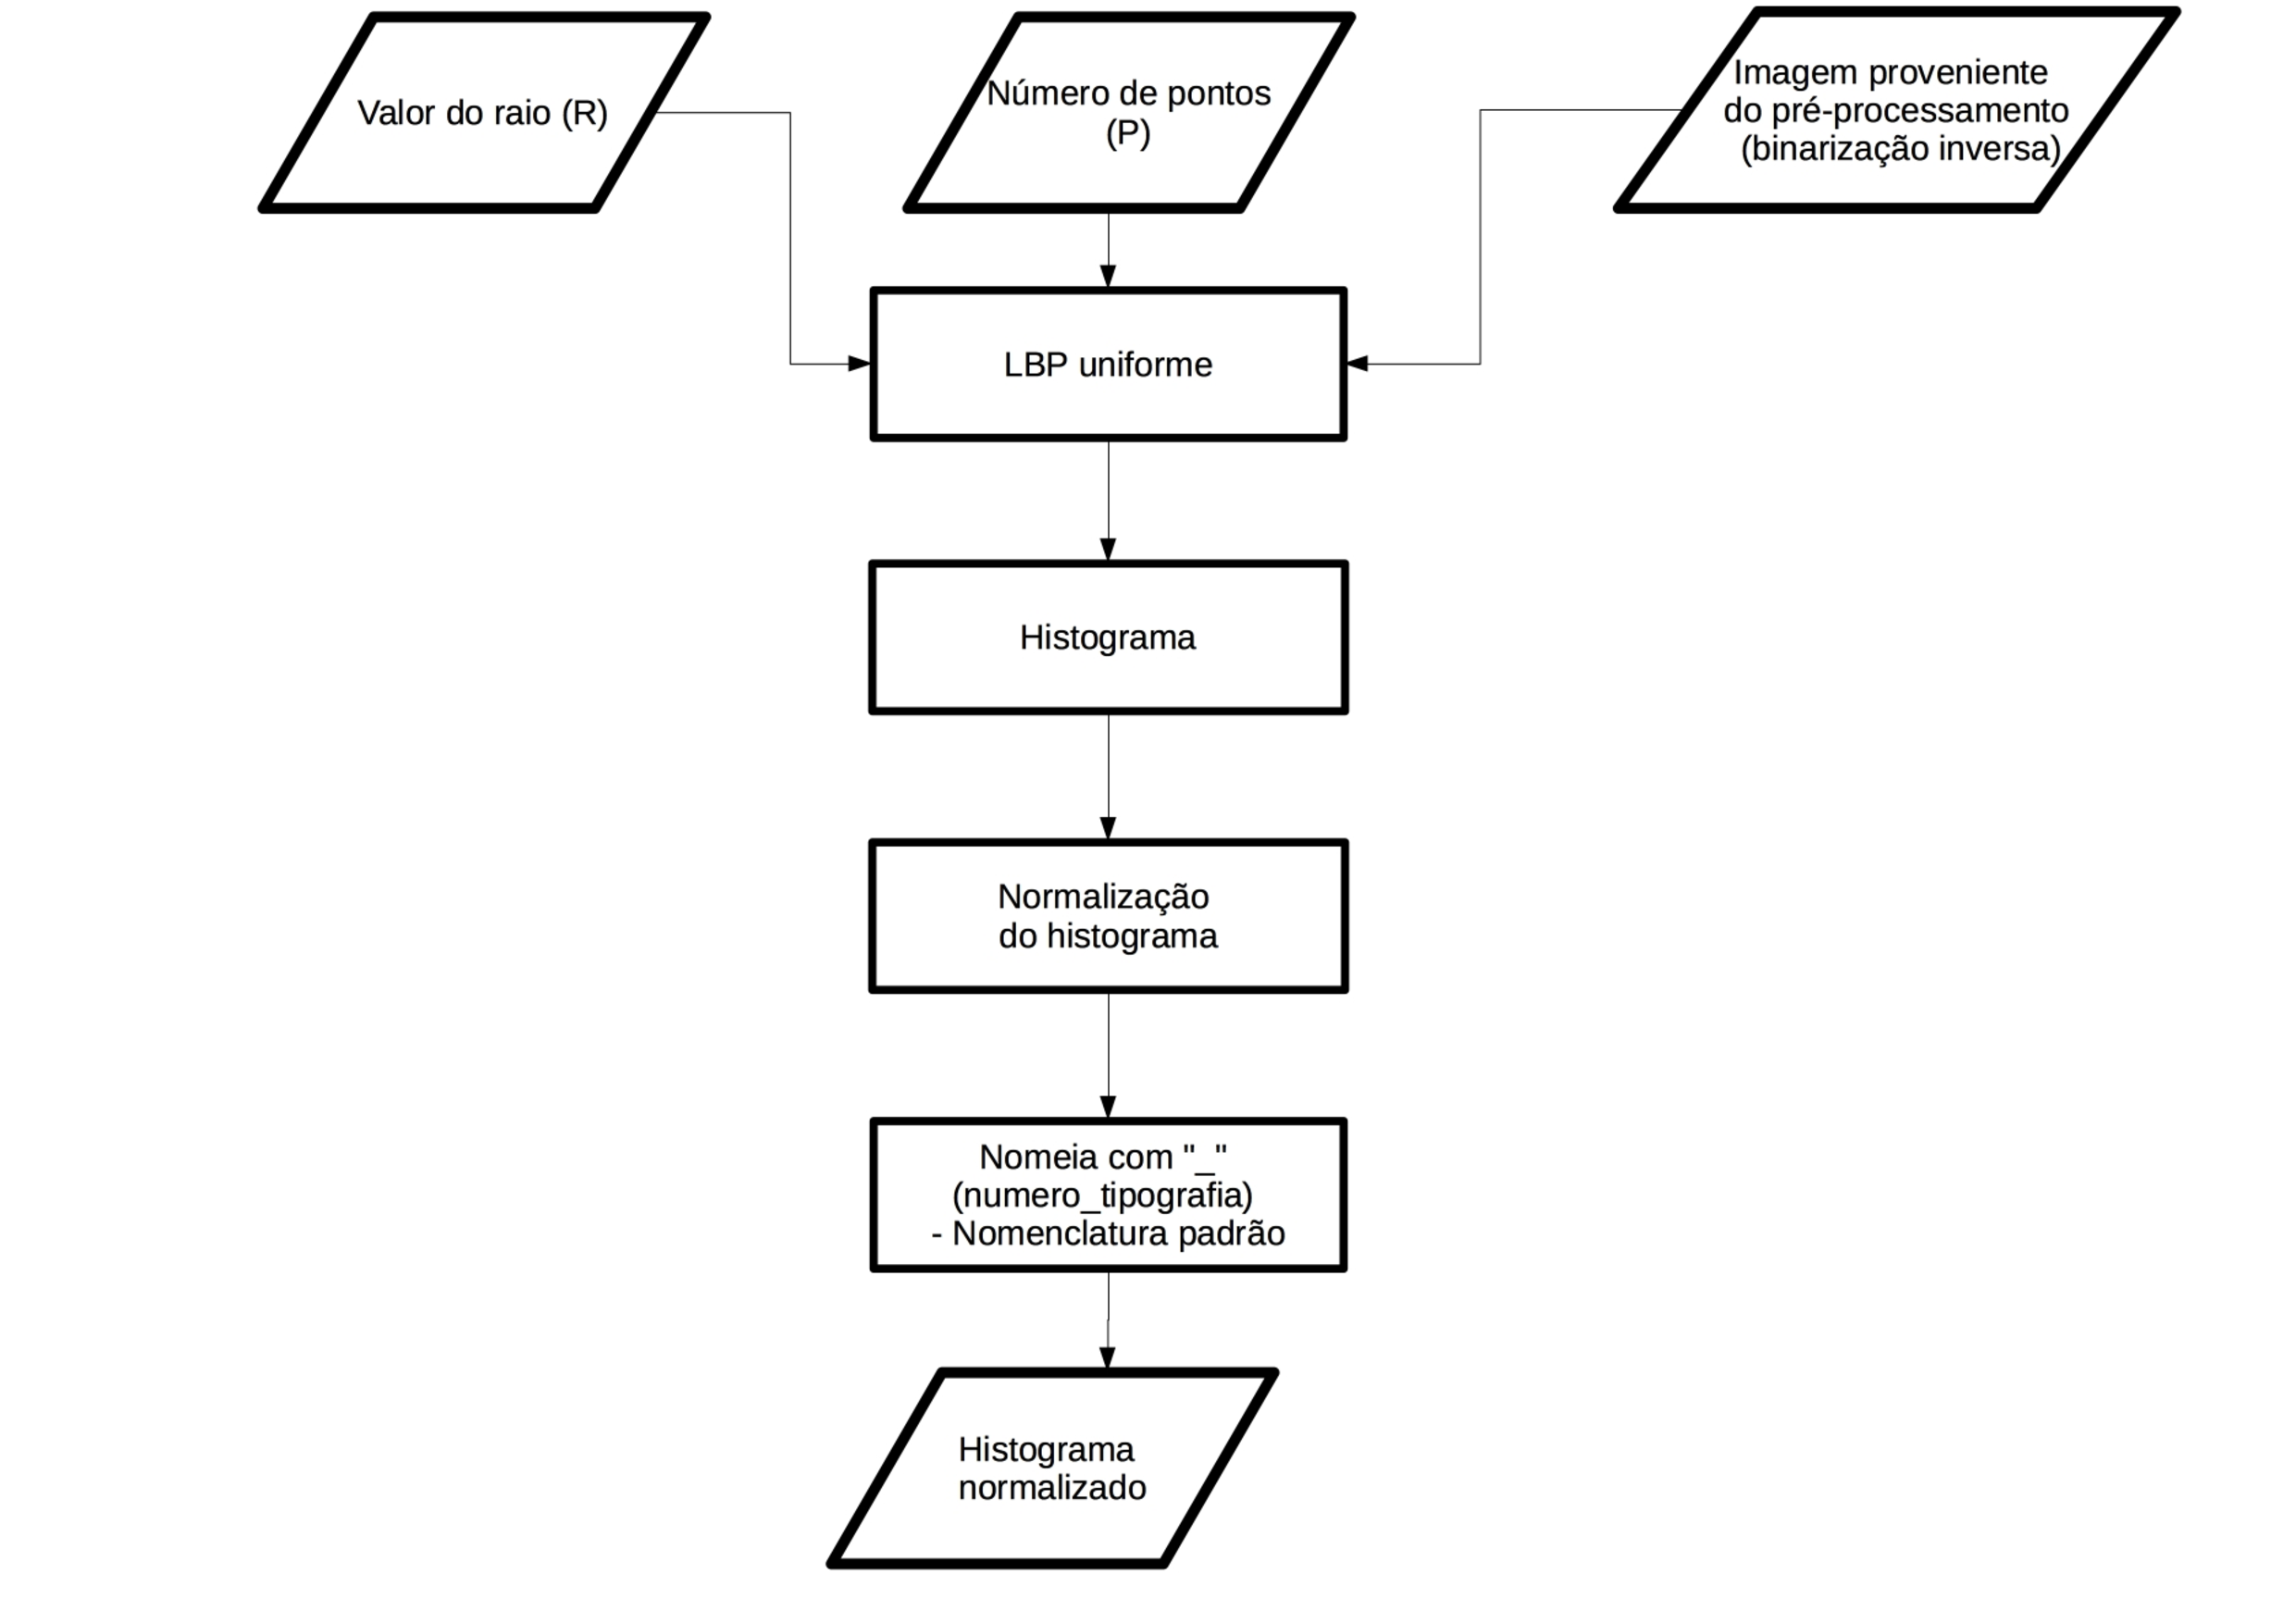
\includegraphics[width=1\linewidth]{figuras/lbp.pdf}
  \caption{Fluxograma do método \texttt{describe} para computar o LBP de uma imagem, retornando seu histograma normalizado.}
  \label{fig:flowLBP}
\end{figure}

Utilizando-se a biblioteca \textit{NumPy} para a estruturação e a manipulação dos vetores de atributos, o histograma da representação da imagem em LBP é então computado e normalizado. O resultado de todo esse processo aplicado às amostras de imagens do banco de imagens é apresentado na Figura \ref{fig:nlbp}. Na Figura \ref{fig:nbinario}, são apresentadas as imagens com binarização inversa, que são as imagens utilizadas como dados de entrada neste estágio (extração de atributos).



A imagem que está sendo analisada segue, então, para a determinação do rótulo referente à sua classe, processo realizado analisando o nome do arquivo. Após isso, o histograma normalizado do LBP, proveniente da extração de atributos, é armazenado em uma lista, denominada Lista de Dados. Em seguida, o rótulo é também armazenado em uma lista, denominada Lista de Rótulos, sendo relacionado ao histograma (representativo dos atributos) por partilharem de mesma posição nas listas de armazanamento. Esse processo é repetido a cada imagem. Toda essa etapa é descrita no fluxograma da Figura \ref{fig:flowtreinamento1}

\begin{figure}[H]
  \centering
  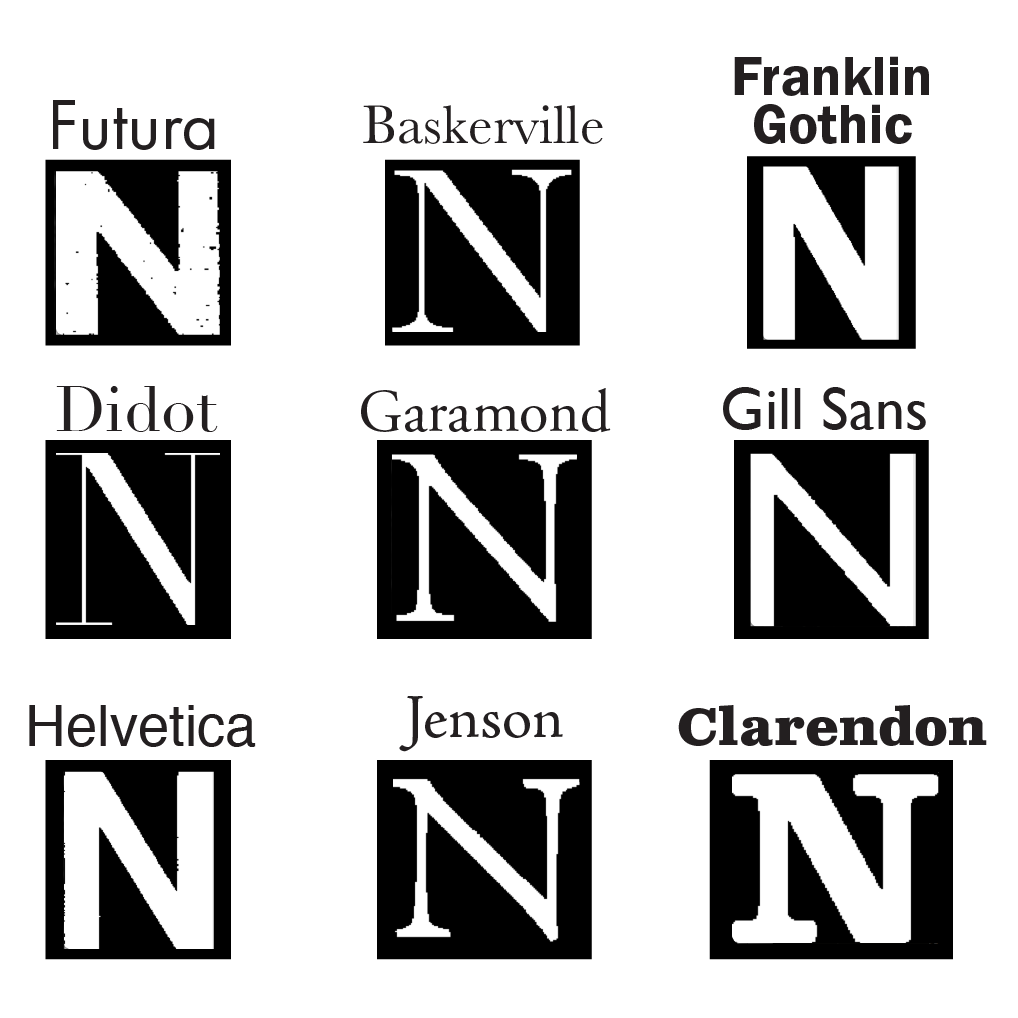
\includegraphics[width=0.4\linewidth]{figuras/nbinario.pdf}
  \caption{Amostras de imagens do banco de imagens após processo de binarização inversa. Imagens de entrada no estágio de extração de atributos.}
  \label{fig:nbinario}
\end{figure}


\begin{figure}[H]
  \centering
  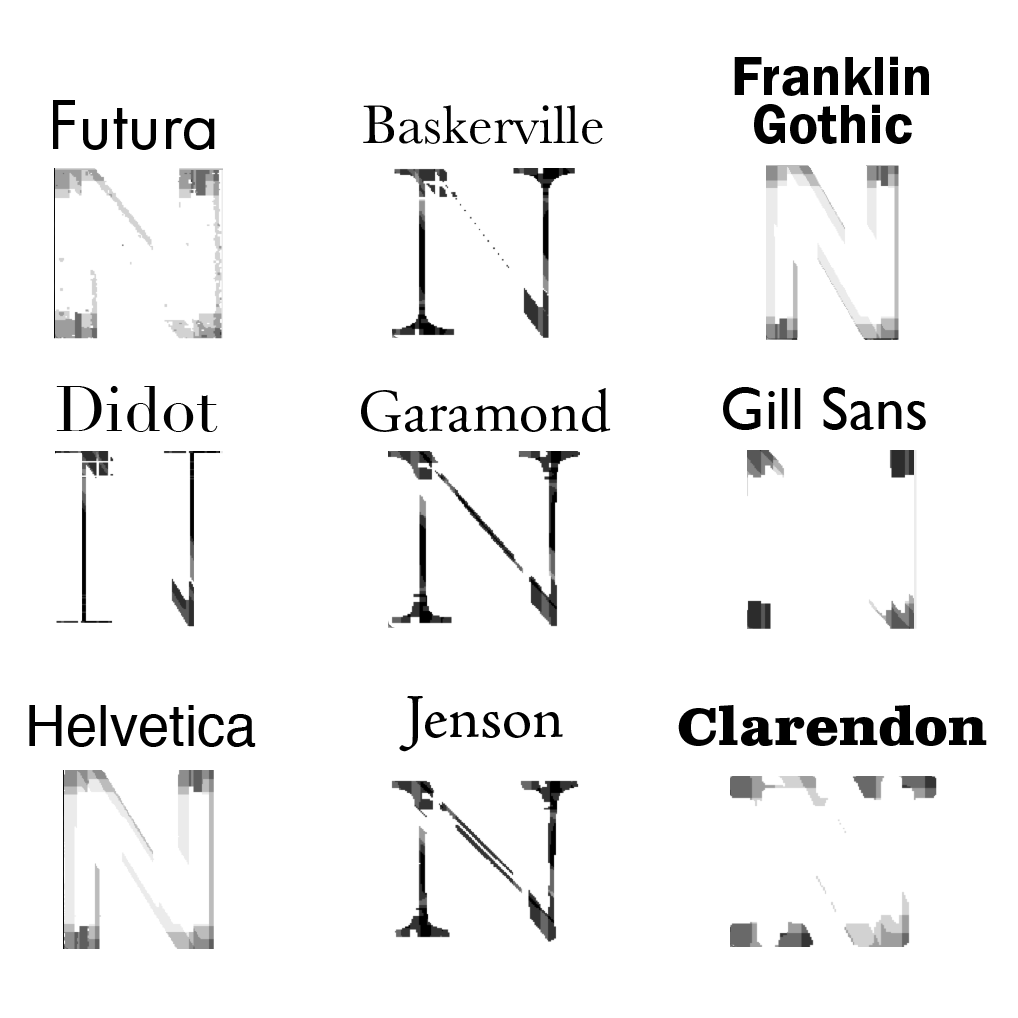
\includegraphics[width=0.4\linewidth]{figuras/enelbp.pdf}
  \caption{Amostras de imagens do banco de imagens após processo de extração de atributos, aplicação do LBP.}
  \label{fig:nlbp}
\end{figure}

Para tornar o processamento mais eficiente, a Lista de Rótulos obtida a partir das imagens é convertida para uma lista formada por inteiros, na qual cada número representa uma classe.

Sendo assim, os elementos de saída deste estágio de extração de atributos são duas listas de dados: uma referente aos rótulos de cada imagem (Lista de Rótulos) e outra, aos histogramas provenientes do LBP (Lista de Dados). São essas duas listas que irão servir de dados de entrada para o estágio de treinamento do modelo.


\begin{figure}[H]
  \centering
  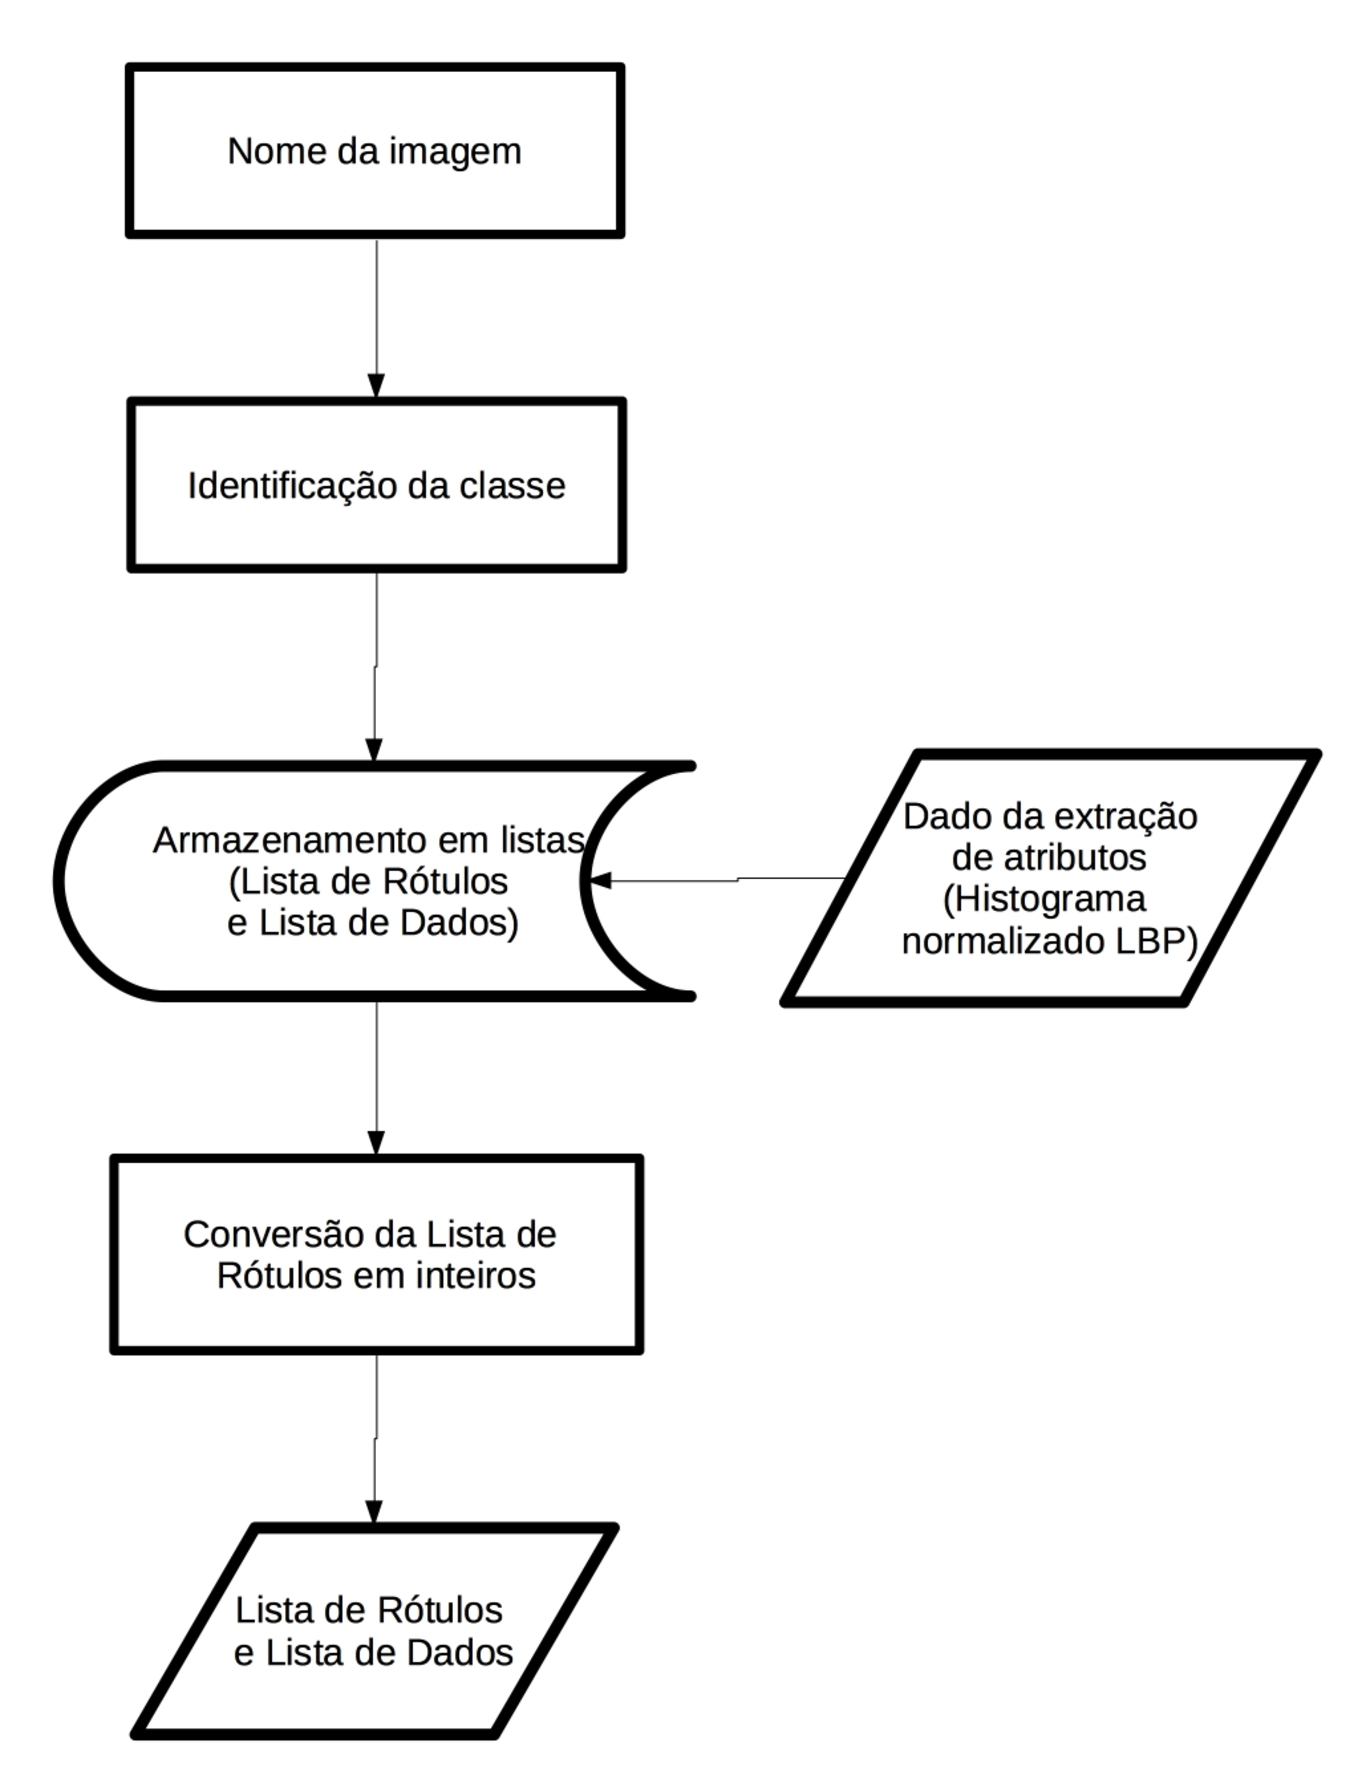
\includegraphics[width=0.55\linewidth]{figuras/treinamento1.pdf}
  \caption{Fluxograma da formação da Lista de Dados e da Lista de Rótulos, ambas dados de entrada para o treinamento do modelo.}
  \label{fig:flowtreinamento1}
\end{figure}


%‘uniform’: improved rotation invariance with uniform patterns and finer quantization of the angular space which is gray scale and rotation invariant.

\subsection{Estágio de treinamento do modelo classificador e testes de predição}

Para o algoritmo desta etapa, a principal biblioteca utilizada foi a \textit{SciKit-learn}, que disponibiliza uma série de ferramentas para várias etapas pertinentes ao aprendizado de máquina. Os módulos utilizados, sendo eles \texttt{svm}, \texttt{ensemble}, \texttt{model\_selection}, \texttt{preprocessing}, oferecem os dois classificadores empregados, métricas para a escolha do modelo e outras ferramentas auxiliares, como a validação cruzada (\textit{Cross Validation}). Todo o processo do estágio de treinamento do classificador e testes de predição é descrito no fluxograma da Figura \ref{fig:flowtreinamento2}.



Nesta etapa, dois modelos foram usados para a classificação das imagens. Primeiramente, utilizou-se o classificador SVM, variando a função \textit{kernel}, a saber, em suas versões Linear, RBF, Sigmoidal e Polinomial. Porém, por apresentar, em todas as alternativas, um índice de acerto de classificação considerado baixo para a aplicação, fato explicitado no próximo capítulo, um novo modelo classificador foi adotado, a Floresta Aleatória.

Para o caso da SVM, foram fornecidos ao modelo alguns parâmetros para sua estruturação, nesse caso, o parâmetro de penalidade \textit{C} do termo erro na classificação, adotado como 100 (o inverso do multiplicador de Lagrange), e o estado randômico (\textit{random state}) para o embaralhamento das imagens, adotado o valor unitário. Além disso, aplicando-se a SVM em uma multiclassificação, utilizou-se a abordagem um-contra-todos, ou seja, são treinados nove classificadores binários, em que uma tipografia é treinada como uma classe e as demais oito tipografias, como a outra classe. Para a classificação de uma nova amostra, são aplicados os nove classificadores binários, aquele que apresenta maior valor, é escolhido como a classe desta imagem.

Para o caso da Floresta Aleatória, os parâmetros fornecidos são o número de árvores de decisão (utilizou-se 82) e o número de tarefas que irão ser realizadas em paralelo (ajustou-se para a execução de número máximo de tarefas em paralelo).

Após isso, passa-se para o ajuste dos parâmetros da validação cruzada a ser utilizada, no caso \textit{Stratified K Fold}. Utilizando essa implementação de validação cruzada, uma variação do modelo \textit{K Fold},  no processo de divisão em subconjuntos (pastas), a porcentagem de amostras de cada classe é mantida de acordo com o conjunto original das imagens. Os parâmetros referentes à validação cruzada utilizada são o número de subconjuntos em que as imagens serão divididas, adotado como sete neste projeto, a opção de embaralhamento e, como no classificador, o estado randômico para o embaralhamento, no qual foi usado valor unitário.

\begin{figure}[H]
 \centering
  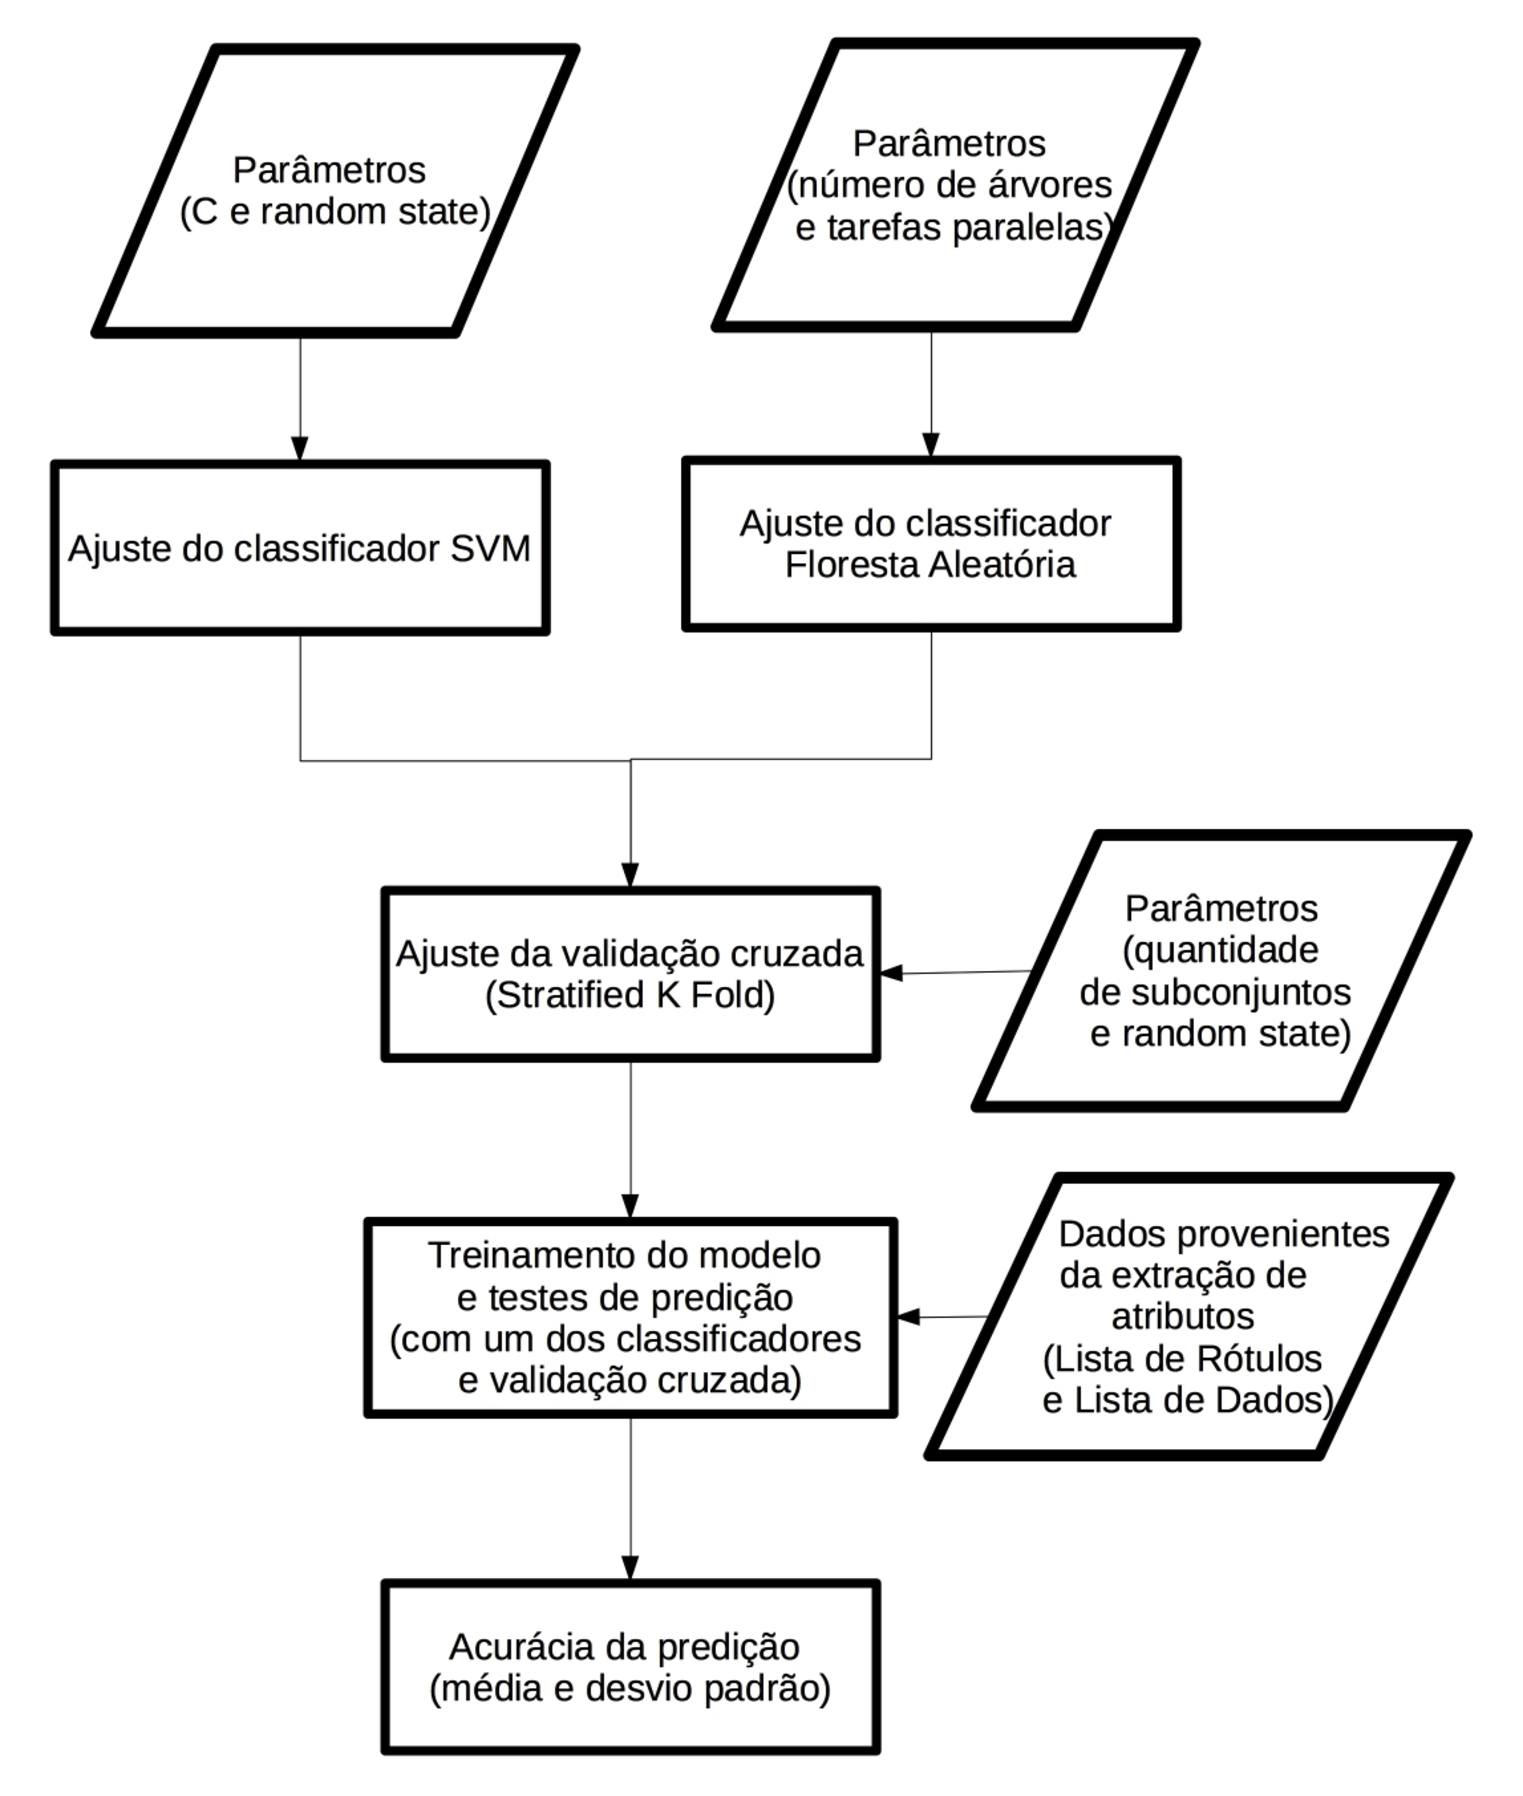
\includegraphics[width=0.6\linewidth]{figuras/treinamento2.pdf}
  \caption{Fluxograma da segunda parte do treinamento do modelo classificador, do ajuste dos modelos classificadores ao resultado de acurácia das predições.}
  \label{fig:flowtreinamento2}
\end{figure}

Em sequência, o classificador é aplicado no conjunto de imagens, o processo se dá com a utilização da validação cruzada previamente ajustada, nesse caso, o treinamento é realizado e, em seguida, o teste da predição. Baseada em todas as iterações da validação cruzada, a acurácia da classificação é calculada, apresentada como a média e o desvio padrão.


Todo o processo descrito nessa seção foi realizado em várias iterações, com a variação de muitos parâmetros que compõem os modelos para que os valores ótimos fossem encontrados. Todos seus resultados serão apresentados no capítulo seguinte.


%metodologia de outro artigo
%The methodology applied in our processing im- age algorithm was based on to estimate features not over full image, instead of this, feature estima- tionwasdoneoverregionsofimagescalled‘‘sub- image’’.Theestimatedattributearraysofeach sub-image were the reference database to recognize thetypeofeachfont(100windowsaretakenran- domlyovereachfulltext) \citeC{aviles2005}


%A \textit{NumPy} foi ainda utilizada no desenvolvimento das duas bibliotecas \textit{SciKit} aqui empregadas. No escopo do algoritmo desenvolvido para o treinamento do modelo de classificação das tipografias, a \textit{NumPy} foi empregue, principalmente, na etapa de pré-processamento e extração de atributos das imagens.




\chapter{Resultados e Discussão}

Este capítulo é destinado à exposição dos resultados do sistema de classificação de tipografias, contendo a análise e discussão destes no caso da utilização dos dois diferentes modelos classificadores, SVM e \textit{Random Forest}.

\section{Classificação das Tipografias}

O sistema desenvolvido deve receber uma imagem e indicar a qual tipografia o caractere presente na imagem pertence, dentre aquelas escolhidas para compor o projeto. Sendo assim, as possíveis classes para as imagens são:

\begin{enumerate}
\item Adobe Jenson
\item Adobe Garamond
\item Baskerville
\item Didot
\item Clarendon Bold
\item Franklin Gothic URW Demi
\item Helvetica
\item Futura Book
\item Gill Sans
\end{enumerate}

Como descrito no capítulo anterior, o resultado da classificação das tipografias foi mensurado a partir de testes de predição utilizando validação cruzada e computando sua acurácia variadas vezes. Além disso, o sistema foi sendo desenvolvido com o banco de imagens sendo incrementado de tipografia a tipografia e, em cada passo, realizada a validação cruzada e os testes de predição, bem como calculada a acurácia desse estágio. Todos esses dados são explicitados nas seções a seguir.

\subsection{Utilizando Support Vector Machine}

Primeiramente, utilizou-se para extração de atributos o modelo LBP e, para o classificador, o modelo linear SVM. Na tabela \ref{tab:svmResults} pode-se verificar o resultado de acurácia obtido mediante a utilização de banco de imagens de diferentes versões. As tipografias presentes em cada banco de imagens são apresentadas na tabela, iniciando-se somente com \textit{Helvetica} e \textit{Garamond} e prosseguindo a incrementação do banco de imagens, tipografia à tipografia. Além disso, o leitor pode acompanhar na Figura \ref{fig:graficoSVM} o histórico da acurácia do sistema classificador utilizando os modelos citados.

%%% Tabela

\begin{table}[h]
 \centering
 \begin{tabular}{l|c|c|c|c|c|c|c|c|c|c}
    Quantidade de tipografias  & 2 & 3 & 4 & 5 & 6 & 7 & 8 & 9\\ no banco de imagens & & & & & & & & \\
	\hline
	Helvetica & X & X & X & X & X & X & X & X   \\
	Garamond & X & X & X & X & X & X & X & X  \\
	Clarendon &  & X & X & X & X & X & X & X    \\
	Futura &  &  & X & X & X & X & X & X  \\
	Baskerville &  &  &  & X & X & X & X & X    \\
	Didot &  &  &  &  & X & X & X & X    \\
	Gill Sans &  &  &  &  &  & X & X & X   \\
	Jenson &  &  &  &  &  &  & X & X  \\
	Franklin Gothic &  &  &  &  &  &  &  & X  \\
	\hline
	Acurácia [\%] & 94,2 & 83,16 & 64,47 & 57,58 & 55,94 & 50,44 & 48,15 & 45,53 \\
	Desvio padrão [\%] & 2 & 5 & 4 & 5 & 2 & 2 & 3 & 3\\
 \end{tabular}
 \caption{Resultados de acurácia em testes de validação cruzada do sistema classificador utilizando o modelo SVM, avaliado com banco de imagens em processo de incrementação tipografia à tipografia - \textbf{Fonte:} Autora}
 \label{tab:svmResults}
\end{table}

%%% gráfico

\begin{figure}[H]
 \centering
  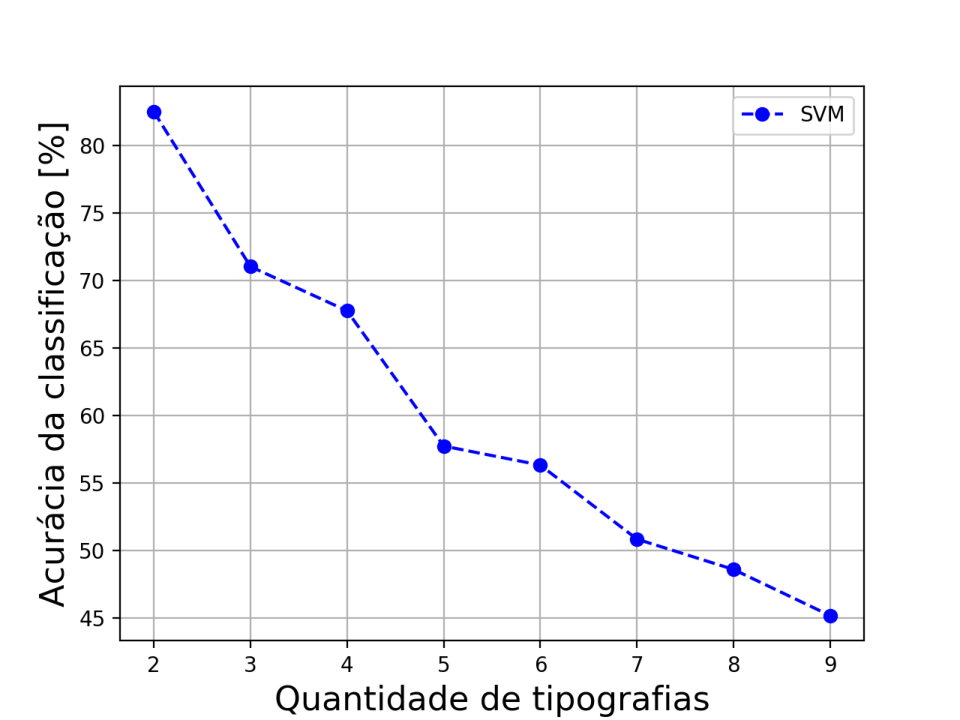
\includegraphics[width=0.7\linewidth]{figuras/graficosvm.pdf}
  \caption{Gráfico do desempenho do sistema classificador com o modelo SVM em relação à quantidade de tipografias presentes no banco de imagens - \textbf{Fonte:} Autora}
  \label{fig:graficoSVM}
\end{figure}

Percebe-se que, a cada incremento no banco de imagens, a acurácia é bastante comprometida, chegando ao baixo índice de 45,53\%, desvio padrão de 3\%, com banco de imagens completo. Diante do nível de acurácia bastante insatisfatório em comparação com trabalhos similares com índices de 85\% e 96,91\%, decidiu-se aplicar outro modelo classificador \citeC{la1999} \citeC{zramdini1998}. O resultado ruim pode ser fruto de uma sensibilidade do modelo SVM quanto aos atributos (dados) que lhe são fornecidos durante a etapa de treinamento \citeC{lorena2007}. Além disso, como já comentado anteriormente, a classificação é dificultada diante do alto grau de similaridade entre algumas tipografias presentes no projeto.

Portanto, para continuar empregando o classificador SVM, um modelo mais robusto de extração de atributos deveria ser utilizado, o que seria também uma opção para implementação do sistema. Porém, optou-se por manter o LBP para extração de atributos devido ao seu baixo custo computacional e rapidez de execução, critério importante no cenário de grande volume de dados e também por ser uma aplicação interativa, em se tratando de um produto final.

É ainda importante enfatizar a influência do conjunto de dados composto para o treinamento e testes no caso de aprendizado de máquina. Como descrito no capítulo anterior, o primeiro banco de imagens criado para treinamento e testes do sistema classificador comprometeu severamente a acurácia da classificação realizada pelo sistema. A Tabela X apresenta uma comparação entre os resultados obtidos com o banco de imagens precedente e o banco de imagens após maior refinamento.

\subsection{Utilizando Random Forest Classifier}

O segundo classificador utilizado foi o \textit{Random Forest Classifier}, ainda com o modelo LBP para extração de atributos das imagens. Assim como na primeira versão do sistema, o modelo classificador foi treinado com oito versões do banco de imagens. A primeira versão é composta de duas tipografias que são suficientemente distintas entre si e então, a cada versão, o banco de imagens é incrementado com um conjunto de imagens de uma das tipografia presentes no projeto. Os resultados de acurácia da classificação performada pelo sistema utilizando \textit{Random Forest} como classificador são expostos na Tabela \ref{tab:rfcResults} e, na Figura \ref{fig:grafico2}, pode-se ver a comparação dos resultados do classificador SVM e do classificador \textit{Random Forest} a medida em que o banco de imagens foi sendo incrementado.


%%% Tabela

\begin{table}[h]
 \centering
 \begin{tabular}{l|c|c|c|c|c|c|c|c|c|c}
    Quantidade de tipografias  & 2 & 3 & 4 & 5 & 6 & 7 & 8 & 9\\ no banco de imagens & & & & & & & & \\
	\hline
	Helvetica & X & X & X & X & X & X & X & X   \\
	Garamond & X & X & X & X & X & X & X & X  \\
	Clarendon &  & X & X & X & X & X & X & X    \\
	Futura &  &  & X & X & X & X & X & X  \\
	Baskerville &  &  &  & X & X & X & X & X    \\
	Didot &  &  &  &  & X & X & X & X    \\
	Gill Sans &  &  &  &  &  & X & X & X   \\
	Jenson &  &  &  &  &  &  & X & X  \\
	Franklin Gothic &  &  &  &  &  &  &  & X  \\
	\hline
	Acurácia [\%] & 99,27 & 95,38 & 91,54 & 87,82 & 87,96 & 85,09 & 85,03 & 84,87 \\
	Desvio padrão [\%] & 0 & 2 & 1 & 3 & 2 & 3 & 2 & 3\\
 \end{tabular}
 \caption{Resultados de acurácia em testes de validação cruzada do sistema com o modelo Random Forest, avaliado com banco de imagens em processo de incrementação tipografia à tipografia - \textbf{Fonte:} Autora}
 \label{tab:rfcResults}
\end{table}


%%% gráfico

\begin{figure}[H]
 \centering
  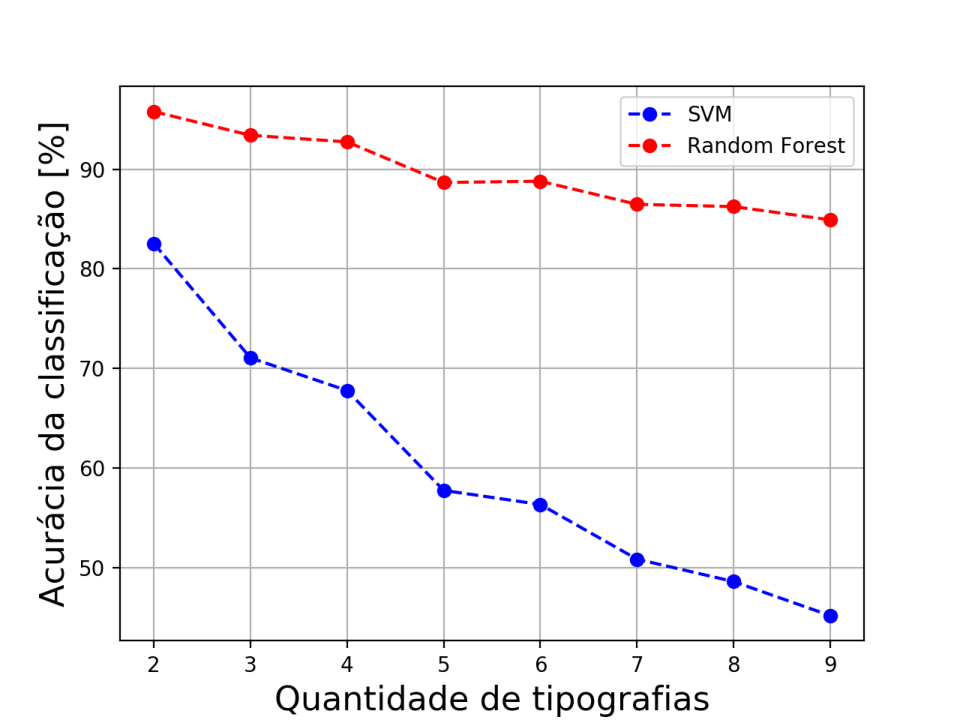
\includegraphics[width=0.7\linewidth]{figuras/graficosvmrfc.pdf}
  \caption{Gráfico do desempenho do sistema classificador com os dois modelos utilizados, SVM e \textit{Random Forest}, em relação à quantidade de tipografias presentes no banco de imagens - \textbf{Fonte:} Autora}
  \label{fig:grafico2}
\end{figure}

Sendo assim, o resultado final obtido para a classificação das nove tipografias apresentou uma acurácia de 84,87\%, com desvio padrão de 3\%. O desempenho encontrado foi bastante superior ao caso anterior devido à alteração do modelo, elevando a acurácia do sistema classificador a um valor satisfatório. Apesar de ainda ser passível de melhoria, o desempenho foi similar ao encontrado em trabalho semelhante, que apresentou acurácia de 85\%, portanto, suficiente para um primeiro estágio no momento \citeC{la1999}.

Nota-se a grande discrepância entre o desempenho do sistema empregando o classificador \textit{Random Forest} e o SVM. Esse resultado pode ser derivado de vários aspectos, entre eles, o perfil do conjunto de dados necessário para garantir um bom funcionamento do SVM como classificador.

O SVM com \textit{kernel} linear foi aquele que obteve melhor resultado apesar de vários treinamentos da máquina terem sido efetuados com outras opções de \textit{kernel}, que podem ser vistos na Tabela \ref{tab:svmkernelResults}. Implementações com modelos não-lineares foram realizados somente no estágio final do banco de imagens, ou seja, com conjunto completo de nove tipografias.

\begin{table}[h]
 \centering
 \begin{tabular}{l|c|c}
    Kernel & Acurácia [\%] & Desvio Padrão [\%]\\
	\hline
	Linear &  45,53 & 3 \\
	RBF & 37,28 & 4 \\
	Polinomial & 18,01 & 6  \\
	Sigmoidal & 35,61 & 5 \\
 \end{tabular}
 \caption{Resultados de acurácia em testes de validação cruzada do sistema com o modelo SVM avaliado com diferentes \textit{kernels} em banco de imagens completo - \textbf{Fonte:} Autora}
 \label{tab:svmkernelResults}
\end{table}

Vale notar que o SVM linear obtém bom desempenho como classificador em conjuntos de dados com distribuição linear, ou que se aproximem desse padrão. Já no caso da utilização de \textit{kernel} não-linear, o conjunto de treinamento é mapeado para um espaço com dimensão superior e que seja mais suscetível à uma separação linear das classes \citeC{lorena2007}.

No entanto, os dois casos possuem um grau de dependência da distribuição do conjunto original de dados para que apresentem bom desempenho na classificação. Além disso, como pode-se perceber por sua característica linear intrínseca, o modelo SVM foi concebido como um classificador binário e, posteriormente, adaptado para conjuntos não-lineares em casos de multi-classificação \citeC{boser1992}. Dessa forma, a utilização do SVM nesse caso depende de uma série de parâmetros que devem ser bem ajustados para que ocorra a separação linear de forma ótima, o que dificulta sua utilização, fator que pode ter sido decisivo em seu desempenho neste projeto.

Em relação ao modelo classificador \textit{Random Forest}, os motivos pelos quais sua aplicação resultou em desempenho satisfatório podem estar relacionados à robustez do modelo em relação à distribuição e características gerais do conjunto de dados de entrada na máquina, já que, para seu bom funcionamento, não depende da linearidade da distribuição dos dados. Além disso, por se tratar de um modelo construído, em sua maioria, por árvores de decisão (\textit{decision trees}), possui uma capacidade ampliada para lidar com espaços de variadas dimensões e também com um número alto de amostras de treinamento. Sendo assim, o \textit{Random Forest} pode ser considerado como um modelo que é intrinsicamente ajustado para multi-classificação, fato que facilita a sua utilização no caso aqui apresentado.

%As SVMs lineares são eficazes na classificação de conjuntos de dados linearmente se- paráveis ou que possuam uma distribuição aproximadamente linear, sendo que a versão de margens suaves tolera a presença de alguns ruídos e outliers. Porém, há muitos casos em que não é possível dividir satisfatoriamente os dados de treinamento por um hiperplano. Um exemplo é apresentado na Figura 8a, em que o uso de uma fronteira curva seria mais adequada na separação das classes. \citeC{lorena2007}

%As SVMs lidam com problemas não lineares mapeando o conjunto de treinamento de seu espaço original, referenciado como de entradas, para um novo espaço de maior dimensão, denominado espaço de características (feature space) [15]. Seja Φ : X → I um mapeamento, em que X é o espaço de entradas e I denota o espaço de características. A escolha apropriada de Φ faz com que o conjunto de treinamento mapeado em I possa ser separado por uma SVM linear. (BOA FIGURA NO ARTIGO)

\chapter{Conclusão}
\label{ch:Conclusao}

Dado que a proposta deste trabalho é desenvolver um sistema de reconhecimento de padrões em tipos para aplicação no projeto de Tipografia Tátil, que tem como objetivo auxiliar o ensino de tipografia a deficientes visuais, nesta monografia foi implementado um sistema capaz de reconhecer a qual tipografia pertence o caractere apresentado em imagem, classificando-o de acordo com as tipografias escolhidas no projeto.

A criação do banco de imagens é uma contribuição para outros projetos de mesma área, já que é uma etapa que, no geral, demanda uma grande quantidade de tempo no processo de desenvolvimento de um projeto de Aprendizado de Máquina. Para o acesso ao banco de imagens completo, tem-se um \textit{link} apresentado no capítulo anterior, bem como o de todos algoritmos desenvolvidos.

Em relação ao produto de tecnologia assistiva como um todo, testes foram feitos com deficientes visuais para ajustes no desenvolvimento das peças táteis. No entanto, em relação ao sistema computacional interativo, foram feitas apenas entrevistas com alguns deficientes visuais. Após o desenvolvimento de mais partes do sistema computacional, é necessário que sejam feitos mais testes para que ajustes possam ser realizados no sistema, de forma a torná-lo de fácil utilização para o usuário.

Como trabalhos futuros, deve-se buscar melhorar o índice de acerto do sistema classificador, de forma a atingir um nível próximo ou superior ao obtido por outros autores \citeC{Zramdini1995}. Para tal, pretende-se tentar uma abordagem parecida com a usada no trabalho citado, criando, para cada letra, um sistema classificador distinto para realizar a OFR.

 O descritor de imagem utilizado, LBP, foi suficiente para a descrição das imagens para esta aplicação. Porém, outra possibilidade é utilizar outros descritores de imagem para a extração de atributos, ou uma combinação, como, por exemplo, um combinação do LBP e HOG (\textit{Histogram of Oriented Gradient}), que apresenta melhor desempenho em variados casos \citeC{zhang2011} \citeC{wang2009}. Ainda, o modelo classificador Floresta Aleatória obteve um índice de acerto de classificação suficiente para primeira versão do sistema, porém pode-se escolher um novo modelo classificador para a implementação para a fase final do trabalho. Por último, pretende-se alimentar o conjunto de dados de treinamento com mais exemplos, o que pode resultar em um melhor desempenho do sistema \citeC{perottoalvares2005}.

Finalmente, para que o sistema esteja completo é necessário implementar o OCR para que o caractere da peça seja reconhecido. É necessário também que todas as funcionalidades do sistema sejam agrupadas. Sendo assim, uma fase de integração dos algoritmos com uma interface para o usuário é necessária. Este passo vai permitir integrar o sistema classificador com a síntese de voz, que vai fornecer os comandos para guiar o usuário e informá-lo segundo material didático já desenvolvido para o projeto \citeC{cruz2017}.



% etc

%%%%%%%%%%%%%%%%%%%%%%%%%%%%%%%%%%%%%%%%%%%%%%%%%%%%%%%%%%%%%%%%%%%%%%%%%
% Referências bibliográficas											%
%%%%%%%%%%%%%%%%%%%%%%%%%%%%%%%%%%%%%%%%%%%%%%%%%%%%%%%%%%%%%%%%%%%%%%%%%
\bibliographystyle{config/abntex2/abntex2-num} % use este estilo para ABNT numérico
%\bibliographystyle{config/abntex2/abntex2-alf} % use este estilo para ABNT alfabético
\renewcommand{\bibname}{REFERÊNCIAS BIBLIOGRÁFICAS}
\phantomsection
\addcontentsline{toc}{chapter}{REFERÊNCIAS BIBLIOGRÁFICAS}
\bibliography{referencias}

%%%%%%%%%%%%%%%%%%%%%%%%%%%%%%%%%%%%%%%%%%%%%%%%%%%%%%%%%%%%%%%%%%%%%%%%%
% Anexos																%
%%%%%%%%%%%%%%%%%%%%%%%%%%%%%%%%%%%%%%%%%%%%%%%%%%%%%%%%%%%%%%%%%%%%%%%%%
%\anexos

\makeatletter % não retirar estes comandos
\renewcommand{\@makechapterhead}[1]{%
  {\parindent \z@ \raggedleft \setfontarial\bfseries
        \LARGE \thechapter. \space\space
    \uppercase{#1}\par
    \vskip 40\p@
  }
}
\makeatother


% *** Anexo I: Diagramas esquemáticos ***
%\include{anexo_Codigosfonte}

%\refstepcounter{noAnexo}

% *** Anexo II: Descrição do CD ***
%\include{anexo_CD}
%\refstepcounter{noAnexo}

%\pdfbookmark[level]{text}{name}
% Acrescente mais anexos conforme julgar necessário.
\end{document}

